\chapter{Các mô hình khả diễn giải}
Cách đơn giản nhất để làm chủ tính khả diễn giải đó là ta chỉ sử dụng một tập nhỏ các thuật toán để tạo ra các mô hình khả diễn giải. Các mô hình như hồi quy tuyến tính, hồi quy logistic và cây quyết định đều có tính khả diễn giải cao.

Trong các mục tới đây, ta sẽ thảo luận về các mô hình này. Tôi không đi sâu vào chi tiết mà chỉ một cách cơ bản, bởi vì đã có rất nhiều tài liệu và sách báo tập trung vào các vấn đề này. Ta sẽ tập trung vào câu hỏi \textit{Làm sao để diễn giải một mô hình?}. Chương này ta thảo luận sâu về tính khả diễn giải của các mô hình \href{TODO}{hồi quy tuyến tính, hồi quy logistic, các dạng mở rộng của hồi quy tuyến tính, cây quyết định, luật quyết định và thuật toán RuleFit}. Cuối cùng, ta cũng sẽ nhắc sơ qua tới \href{TODO}{một vài mô hình khả diễn giải khác}. 

Tất cả các mô hình khả diễn giải trong cuốn sách này được đề cập ở mức độ mô đun, ngoại trừ thuật toán k hàng xóm gần nhất (K-Nearest Neighbors). Bảng dưới đây trình bày một cách tổng quan về các loại mô hình khả diễn giải và các đặc tính của chúng. Một mô hình là tuyến tính nếu mối quan hệ giữa đặc trưng (features) và mục tiêu (target) được mô hình một cách tuyến tính. Một mô hình với tính đơn điệu (monotonicity) luôn đảm bảo rằng mối quan hệ giữa một đặc trưng và kết quả đầu ra luôn luôn đồng biến trên toàn bộ miền đặc trưng: Nếu ta tăng giá trị của một giá trị đặc trưng thì giá trị đầu ra có thể tăng hoặc giảm một cách tương ứng. Tính đơn điệu trở nên hữu ích cho việc diễn giải một mô hình vì các mối quan hệ sẽ dễ dàng được giải thích. Một số mô hình có thể tự động bao gồm các mối tương tác giữa các đặc trưng để dự đoán kết quả. Ta có thể gộp các tương tác giữa các đặc trưng này bằng cách tạo ra các đặc trưng tương tác (interaction features) một cách thủ công - các đặc trưng thể hiện sự tương tác giữa các đặc trưng. Tương tác có thể giúp cải thiện chất lượng của một mô hình, tuy nhiên việc có quá nhiều tương tác hay các tương tác quá phức tạp sẽ làm giảm tính khả diễn giải. Một vài mô hình giải quyết bài toán hồi quy, số khác giải quyết bài toán phân loại, đôi khi giải quyết cả hai.

Từ bảng \ref{tab:4_1}, ta có thể chọn một mô hình khả diễn giải hợp lý cho bài toán của chúng ta, có thể là hồi quy (regr) hoặc phân loại (class): 

\begin{table*}[hbt!]
\centering
\label{tab:my-table_z}
\begin{tabular}{|l|l|l|l|l|}
\hline
Algorithm           & Linear & Monotone & Interaction & Task       \\ \hline
Linear regression   & Yes    & Yes      & No          & regr       \\ \hline
Logistic regression & No     & Yes      & No          & class      \\ \hline
Decision trees      & No     & Some     & Yes         & class,regr \\ \hline
RuleFit             & Yes    & No       & Yes         & class,regr \\ \hline
Naive Bayes         & No     & Yes      & No          & class      \\ \hline
k-nearest neighbors & No     & No       & No          & class,regr \\ \hline
\end{tabular}
\caption{Các mô hình và đặc tính của chúng.}
\label{tab:4_1}
\end{table*}

\section{Hồi quy tuyến tính}
Một mô hình hồi quy tuyến tính dự đoán mục tiêu dựa trên tổng trọng số của các đặc trưng đầu vào. Sự tuyến tính của các mối quan hệ giữa đặc trưng và đầu ra của mô hình khiến cho sự diễn giải trở nên đơn giản. Kiểu mô hình này được sử dụng rộng rãi trong thống kê và khoa học máy tính cũng như các ngành khác khi ta muốn giải quyết các vấn đề mang tính định lượng.

Phương pháp này có thể được sử dụng để mô hình sự phụ thuộc của một mục tiêu hồi quy y vào một số đặc trưng x. Mối quan hệ sau quá trình học là tuyến tính và có thể được biểu diễn như sau: $$y=\beta_{0}+\beta_{1}x_{1}+\ldots+\beta_{p}x_{p}+\epsilon$$

Đáp ứng của mô hình đối với một đầu vào là tổng trọng số của p đặc trưng. Các giá trị beta $\beta_{j}$ biểu diễn các trọng số tương ứng với các đặc trưng hay còn gọi là hệ số (coefficients). Trọng số đầu tiên $\beta_0$ được gọi là hệ số chặn (intercept) và không được nhân với đặc trưng. Giá trị epsilon $\epsilon$ là sai số, ví dụ sự khác nhau giữa dự đoán và giá trị thực tế. Lượng sai số này được giả định tuân theo phân phối Gaussian, nghĩa là ta tạo ra sai số theo cả 2 chiều âm dương và có nhiều sai số nhỏ bên cạnh rất ít sai số có giá trị lớn (tuân theo phân bố dạng hình chuông của Gaussian).

Các phương pháp dùng để ước tính giá trị trọng số tối ưu rất đa dạng. Một phương pháp đơn giản nhất đó là phương pháp sai số bình phương tối thiểu thường được dùng để tìm ra tập trọng số tối ưu dựa trên sai lệch bình phương giữa giá trị thực tế và dự đoán.
$$\hat{\boldsymbol{\beta}}=\arg\!\min_{\beta_0,\ldots,\beta_p}\sum_{i=1}^n\left(y^{(i)}-\left(\beta_0+\sum_{j=1}^p\beta_jx^{(i)}_{j}\right)\right)^{2}$$

Ta sẽ không thảo luận chi tiết cách để tìm ra các trọng số tối ưu này, tuy nhên, nếu bạn muốn có thể đọc chương 3.2 trong cuốn "The Elements of Statistical Learning" hoặc các bài giảng online về mô hình hồi quy tuyến tính.

Lợi thế lớn nhất của các mô hình hồi quy tuyến tính đó chính là tính tuyến tính: Nó làm cho việc ước lượng kết quả trở nên đơn giản, và quan trọng hơn cả, các phương trình tuyến tính này tạo nên việc diễn giải dễ dàng ở mức mô đun (các trọng số). Đây là một trong những lý do chính tại sao mô hình tuyến tính và các mô hình tương tự được ưa chuộng trong các ngành khoa học như y học, xã hội học, tâm lý học, và rất nhiều các ngành nghiên cứu định lượng khác. Ví dụ, trong y học, ta không chỉ quan tâm đến kết quả dự đoán trên một bệnh nhân mà còn phải định lượng tác động của thuốc dựa trên độ tuổi, giới tính và các đặc trưng khác nhằm hướng tới tính khả giải thích.

Các trọng số được ước lượng tồn tại trong các khoảng tin cậy (confidence intervals). Một khoảng tin cậy là một dải trọng số bao gồm trọng số ``chính xác'' với một độ tin cậy nhất định. Ví dụ, một khoảng tin cậy tới 95\% của một trọng số có giá trị là 2 có thể rơi vào từ 1 đến 3. Khoảng này có thể được diễn đạt như sau: Nếu ta ước lượng lặp đi lặp lại 100 lần với các mẫu dữ liệu mới, khoảng tin cậy có thể bao gồm giá trị chính xác trong 95/100 trường hợp, giả sử rằng mô hình ta đang có hoạt động chính xác trên tập dữ liệu cho trước.

Để đánh giá liệu một mô hình có hoạt động chính xác trên tập dữ liệu hay không sẽ phụ thuộc vào liệu mối quan hệ trong dữ liệu có thỏa mãn một số tiêu chí cụ thể: tính tuyến tính (linearity), tính chuẩn (normality),  hiệp phương sai đồng nhất (homoscedasticity), tính độc lập (independence), các đặc trưng cố định (fixed features), và sự bất tương quan (absence of multicollinearity).

\paragraph{Tính tuyến tính}
Mô hình hồi quy tuyến tính có đầu ra là một tổ hợp tuyến tính của các đặc trưng, điều này vừa là điểm mạnh cũng vừa là hạn chế lớn nhất của loại mô hình này. Tính tuyến tính giúp mô hình khả diễn giải. Các kết quả tuyến tính có thể dễ dàng được định lượng và mô tả. Vì chúng được xây dựng trên phép lấy tổng, ta có thể dễ dàng tách bạch kết quả. Nếu ta nghi ngờ sự tương tác giữa các đặc trưng hoặc quan hệ phi tuyến của một đặc trưng với kết quả cuối cùng, ta có thể thêm các thành phần tuyến tính khác hoặc sử dụng các hàm hồi quy.

\paragraph{Tính chuẩn}
Khi biết trước các đặc trưng, ta giả thiết rằng giá trị đầu ra của mô hình sẽ tuân theo phân phối chuẩn (hay phân phối Gaussian). Nếu giả thiết này không chính xác, khoảng tin cậy mà ta ước lượng của các trọng số cũng sẽ không chính xác.

\paragraph{Hiệp phương sai đồng nhất} (phương sai bất biến)
Trước tiên hãy giải thích phương sai (variance): Đó là sự sai lệch giữa các lần dự đoán trong khi đó độ chệch (bias) là sự sai lệch giữa các lần dự đoán với giá trị thực tế (ground-truth).
Phương sai của các thành phần sai số được giả thiết là bất biến trên cả không gian đặc trưng. Giả sử ta muốn dự đoán giá của một ngôi nhà dựa vào diện tích được đo đạc bởi mét vuông ($m^2$), ta dùng một mô hình tuyến tính và giả thiết rằng, với mọi giá trị diện tích, sai số của các dự đoán sẽ có cùng phương sai. Giả thiết này thường không đúng trong thực tế. Trong ví dụ trên, một căn nhà lớn sẽ có phương sai lớn, bởi vì giá nhà sẽ lớn và thường số phòng của ngôi nhà cũng sẽ ảnh hưởng tới giá trị của nó. Nếu cho rằng sai số trung bình (sự chênh lệch giữa giá trị thực tế và giá trị dự đoán) trong mô hình tuyến tính ta đang có là 50,000 Euros, khi mô hình có tính chất hiệp phương sai đồng nhất, sai số 50,000 này sẽ không đổi với ngôi nhà giá 1 triệu và ngôi nhà giá chỉ 40,000. Điều này là phi lý bởi vì có thể tồn tại giá trị âm cho ngôi nhà.

\paragraph{Tính độc lập}
Ta giả sử rằng các mẫu dữ liệu đầu vào là độc lập với nhau. Nếu ta thực hiện đo đạc lặp đi lặp lại, ví dụ như thử máu nhiều lần trên một bệnh nhân, các mẫu dữ liệu sẽ không độc lập. Với các dữ liệu phụ thuộc, ta cần một mô hình hồi quy tuyến tính đặc biệt, ví dụ như các mô hình hỗn hợp hoặc phương trình ước lượng tổng quát (GEE - generalized estimating equation). Nếu ta chỉ sử dụng mô hình hồi quy tuyến tính thông thường, ta có thể thu được kết quả sai từ mô hình.

\paragraph{Đặc trưng cố định}
Các đặc trưng đầu vào được coi là cố định. ``Cố định'' ở đây có nghĩa là chúng được coi như các hằng số chứ không phải là các biến số thống kê. Điều này có nghĩa là chúng không ảnh hưởng đến sai số của các phép đo. Giả thiết này cũng không thực tế. Tuy vậy nếu không có giả thiết này, ta sẽ phải điều chỉnh mô hình rất phức tạp khi mà ta phải tính toán sai số của các đặc trưng đầu vào, và thường ta sẽ không muốn làm vậy. 

\paragraph{Sự bất tương quan}
Ta không muốn các đặc trưng tương quan mật thiết với nhau, bởi vì điều này sẽ gây khó khăn trong việc tìm ra trọng số tối ưu cho mô hình. Nếu hai đặc trưng tương quan chặt chẽ với nhau, bởi vì giá trị đầu ra là tổng các trọng số của các đặc trưng, ta sẽ không thể biết được đặc trưng nào (1 trong 2) ảnh hưởng đến giá trị dự đoán.

\subsection{Sự diễn giải}
Sự diễn giải của một mô hình hồi quy tuyến tính phụ thuộc vào loại đặc trưng mà nó học:
\begin{packed_enum}
    \item Đặc trưng dạng số: Việc tăng giá trị của một đặc trưng làm thay đổi giá trị đầu ra bởi các trọng số của nó. Một đặc trưng ví dụ đó là diện tích của một ngôi nhà.
    \item Đặc trưng dạng nhị phân: Đặc trưng chỉ mang 1 trong 2 giá trị cho trước, 1 ví dụ đó là đặc trưng ``Nhà có vườn không?'' trong ví dụ giá nhà ở trên. 1 trong 2 giá trị được coi là giá trị tham chiếu (trong một số ngôn ngữ lập trình sẽ có giá trị là 0), ví dụ như ``Không có vườn''. Việc thay đổi giá trị từ giá trị tham chiếu thành giá trị còn lại sẽ ảnh hưởng tới đầu ra của mô hình.
    \item Đặc trưng dạng hạng mục: Trong loại này, một đặc trưng sẽ có thể rơi vào 1 số giá trị nhất định. Ví dụ như đặc trưng ``loại sàn'' có thể có các giá trị như ``thảm'', ``gỗ ép'' và ``gỗ''. Một cách để giải quyết loại dữ liệu này đó là sử dụng biểu diễn one-hot (one-hot encoding). Với 1 đặc trưng hạng mục có $L$ giá trị khả dĩ, ta sẽ chỉ cần $L-1$ cột, bởi vì cột thứ $L$ sẽ bao gồm thông tin không cần thiết (ví dụ khi cột từ 1 đến $L-1$ có tất cả các giá trị là 0, ta sẽ biết rằng giá trị còn lại sẽ phải là 1). Sự diễn giải cho từng mục sẽ giống với sự diễn giải đối với đặc trưng nhị phân. Trong nhiều ngôn ngữ lập trình, ví dụ như R, ta được phép mã hóa các đặc trưng hạng mục theo rất nhiều cách khác nhau, sẽ được thảo luận kĩ hơn trong mục \ref{encoding_cat_features}.
    \item Hệ số chặn $\beta_0$: Hệ số chặn là một trọng số của một đặc trưng bất biến (giá trị của đặc trưng luôn là 1 với mọi điểm dữ liệu đầu vào). Hầu hết các gói phần mềm đều tự động thêm đặc trưng bất biến này để ước lượng giá trị của hệ số chặn. Khi đó, sự diễn giải sẽ là như sau: Với một đầu vào có tất cả các đặc trưng dạng số có giá trị bằng 0 và biến hạng mục có giá trị tại giá trị tham chiếu, dự đoán của mô hình sẽ chính là giá trị của hệ số chặn. Sự diễn giải của hệ số chặn sẽ không mang nhiều ý nghĩa bởi các điểm dữ liệu đầu vào có giá trị đặc trưng là 0 thường không mang thông tin. Việc diễn giải chỉ có ý nghĩa khi mà các đặc trưng được chuẩn hóa (trung bình tại 0 và độ lệch chuẩn là 1). Khi này, hệ số chặn phản ánh giá trị được dự đoán ứng với một điểm dữ liệu đầu vào khi mà tất cả các đặc trưng đều nằm ở giá trị trung bình của chúng.
    
\end{packed_enum}
    
Việc diễn giải đối với các đặc trưng trong mô hình hồi quy tuyến tính có thể rơi vào một trong các trường hợp sau.

\paragraph{Diễn giải một đặc trưng dạng số} Khi ta tăng giá trị của đặc trưng $x_{k}$ một đơn vị, giá trị đầu ra y cũng sẽ tăng 1 lượng $\beta_k$ khi tất cả giá trị của các đặc trưng còn lại được giữ nguyên.

\paragraph{Diễn giải một đặc trưng dạng hạng mục} Việc thay đổi đặc trưng $x_{k}$ từ hạng mục tham chiếu  sang một hạng mục khác sẽ làm tăng giá trị đầu ra y dựa trên $\beta_k$ khi các đặc trưng khác được giữ nguyên.

Một phép đo đạc quan trọng khác cho các mô hình tuyến tính được gọi là phép đo bình phương R (R-squared measurement). Bình phương R hay R-squared cho ta biết được lượng phương sai có thể được giải thích bởi mô hình. Giá trị bình phương R càng lớn, mô hình càng giải thích dữ liệu một cách tốt hơn. Công thức để tính toán bình phương R như sau:
$$R^2=1-SSE/SST$$

Trong đó $SSE$ là tổng bình phương của các thành phần lỗi (error terms):
$$SSE=\sum_{i=1}^n(y^{(i)}-\hat{y}^{(i)})^2$$

$SST$ là tổng bình phương của phương sai:
$$SST=\sum_{i=1}^n(y^{(i)}-\bar{y})^2$$

Giá trị $SSE$ cho ta biết lượng phương sai còn lại sau khi khớp một mô hình tuyến tính, và giá trị này được tính toán dựa trên bình phương sai khác giữa giá trị sinh ra bởi mô hình và giá trị thực tế. Trong khi đó $SST$ là tổng phương sai của các giá trị sinh ra bởi mô hình. Ví dụ, mô hình đưa ra 100 dự đoán, khi đó đầu tiên ta tính mean của 100 dự đoán này, sau đó ta tính tổng phương sai. Bình phương R cho ta biết lượng phương sai có thể được giải thích bởi mô hình tuyến tính. Giá trị bình phương R chạy từ 0 (trong trường hợp mô hình không thể giải thích dữ liệu) tới 1 (khi mô hình giải thích được tất cả phương sai trong dữ liệu).

Tuy vậy, bởi vì giá trị bình phương R tăng tỉ lệ với số lượng đặc trưng trong mô hình, thậm chí cả khi chúng không hàm chứa bất kỳ thông tin nào về dự đoán ta nhận được, ta cần sử dụng một công thức bình phương R khác gọi là bình phương R điều chỉnh (adjusted R-squared) để giải quyết vấn đề này, công thức bình phương R mới như sau:

$$\bar{R}^2=1-(1-R^2)\frac{n-1}{n-p-1}$$
trong đó p là số lượng đặc trưng và n là số mẫu của dữ liệu đầu vào cho việc huấn luyện.

Khi giá trị bình phương R nhỏ, việc diễn giải một mô hình thường không có nhiều ý nghĩa bởi vì những mô hình này về cơ bản không giải thích phương sai nhiều. Bất cứ sự diễn giải nào trên các trọng số sẽ trở nên vô nghĩa.

\paragraph{Độ quan trọng của đặc trưng}
Độ quan trọng của một đặc trưng trong một mô hình hồi quy tuyến tính có thể được đo đạc bởi giá trị tuyệt đối từ thống kê t (t-statistics) của nó. Thống kê t là giá trị trọng số ước lượng tỉ lê với độ lệch chuẩn (standard error).

$$t_{\hat{\beta}_j}=\frac{\hat{\beta}_j}{SE(\hat{\beta}_j)}$$

Hãy phân tích xem công thức này nói với ta những gì? Ở tử số, độ quan trọng của một đặc trưng tăng theo giá trị của trọng số. Và ở mẫu số, nếu một trọng số có phương sai càng lớn (đồng nghĩa với sự chắc chắn của giá trị trọng số càng nhỏ), đặc trưng càng ít quan trọng. 

\subsection{Ví dụ}
\begin{table*}[hbt!]
\centering
\begin{tabular}{|l|l|l|l|}
\hline
                          & Weight  & SE    & |t|  \\ \hline
(Intercept)               & 2399.4  & 238.3 & 10.1 \\ \hline
seasonSUMMER              & 899.3   & 122.3 & 7.4  \\ \hline
seasonFALL                & 138.2   & 161.7 & 0.9  \\ \hline
seasonWINTER              & 425.6   & 110.8 & 3.8  \\ \hline
holidayHOLIDAY            & -686.1  & 203.3 & 3.4  \\ \hline
workingdayWORKING DAY     & 124.9   & 73.3  & 1.7  \\ \hline
weathersitMISTY           & -379.4  & 87.6  & 4.3  \\ \hline
weathersitRAIN/SNOW/STORM & -1901.5 & 223.6 & 8.5  \\ \hline
temp                      & 110.7   & 7.0   & 15.7 \\ \hline
hum                       & -17.4   & 3.2   & 5.5  \\ \hline
windspeed                 & -42.5   & 6.9   & 6.2  \\ \hline
days\_since\_2011         & 4.9     & 0.2   & 28.5 \\ \hline
\end{tabular}
\caption{Giá trị trọng số, độ lệch chuẩn và thống kê t của các đặc trưng.}
\label{tab:4_2}
\end{table*}

Trong ví dụ này, ta sẽ sử dụng mô hình hồi quy tuyến tính để dự đoán số lượng xe đạp được thuê trong một ngày nhất định, cho trước điều kiện thời tiết và thông tin về ngày đó trên lịch vạn niên. \textit{Khi nói về diễn giải, ta phân tích các trọng số}. Các đặc trưng bao gồm cả dạng số và dạng hạng mục. Với mỗi đặc trưng, bảng \ref{tab:4_2} cho ta thấy giá trị trọng số được ước lượng, độ lệch của của phép ước lượng (standard error hay SE), và giá trị tuyệt đối của thống kê t ($|t|$).


Sự diễn giải đối với một đặc trưng dạng số (ví dụ như nhiệt độ): Khi giá trị nhiệt độ tăng 1 độ, số lượng xe đạp được dự đoán được thuê sẽ tăng 110.7 xe với điều kiện tất cả các đặc trưng còn lại được giữ nguyên.

Sự diễn giải của một đặc trưng hạng mục (weathersit): Số xe sẽ giảm đi 1901.5 nếu trời mưa, tuyết rơi hoặc bão, so với điều kiện thời tiết tốt (vẫn trong điều kiện là các đặc trưng còn lại được giữ nguyên). Khi thời tiết nhiều sương mù, số lượng xe được dự đoán sẽ nhỏ hơn 379.4 xe so với trong điều kiện thời tiết tốt, giả sử tất cả các đặc trưng còn lại không đổi.

Mọi sự diễn giải luôn cần điều kiện đó là ``các đặc trưng còn lại được giữ nguyên''. Điều kiện này cần được đảm bảo vì đây là bản chất của các mô hình hồi quy tuyến tính. Giá trị được dự đoán là một tổ hợp tuyến tính của các trọng số và đặc trưng. Công thức tuyến tính này biểu diễn một siêu phẳng (hyperplane) trong không gian đặc trưng (nếu chỉ có một đặc trưng nó sẽ là 1 đường). Các trọng số này sẽ xác định gradient của siêu phẳng theo từng hướng khác nhau. Ưu điểm đó là các phép cộng sẽ cho phép ta phân tách sự diễn giải của một đặc trưng với các đặc trưng còn lại bởi vì giá trị cuối cùng là một tổng dựa trên các trọng số và các giá trị đặc trưng. Tuy nhiên, nhược điểm của việc này đó là việc diễn giải sẽ bỏ qua mối liên hệ giữa các đặc trưng. Khi ta tăng giá trị của một đặc trưng, nhưng giữ nguyên đặc trưng còn lại, giá trị đầu vào có thể rơi vào vùng dị thường hoặc giá trị này biến thành giá trị ngoại lai. Ví dụ, khi ta tăng số phòng, diện tích của căn nhà cũng nên được cân nhắc để được tăng theo.

\subsection{Diễn giải trực quan}
Ta có rất đa dạng các phương pháp trực quan hóa để giúp diễn giải một mô hình hồi quy tuyến tính.

\subsubsection{Phác họa trọng số}
Từ thông tin ta có trong bảng trọng số \ref{tab:4_2} (giá trị của trọng số và phương sai) có thể được biểu diễn như trong hình duới đây:

\begin{figure*}[hb!]
	\centering
	\includegraphics[scale=0.23]{images/linear-weights-plot-1.png}
	\label{fig:4_1_3_1}
	\caption{Giá trị các trọng số được hiển thị tương ứng với các điểm và khoảng tin cậy 95\% tương ứng với các đường.}
\end{figure*}

Việc phác họa trọng số cho ta thấy điều kiện thời tiết (mưa/tuyết rơi/có bão) sẽ có tác động tiêu cực lớn tới số lượng xe được thuê. Trong khi đó, giá trị trọng số của đặc trưng ``the working day'' gần với 0 và 0 được bao gồm trong cả khoảng 95\%, nghĩa là ảnh hưởng của đặc trưng này không lớn về mặt thống kê. Một số khoảng tin cậy có giá trị rất nhỏ và các ước lượng gần với giá trị 0, tuy nhiên các ảnh hưởng đặc trưng lại mang nhiều ý nghĩa về mặt thống kê. Nhiệt độ là một ví dụ nổi bật. Vấn đề của việc phác họa trọng số đó là các đặc trưng được đo đạc ở các dải giá trị khác nhau. Với thời tiết thì các trọng số biểu thị sự khác nhau giữa thời tiết tốt và thời tiết xấu, trong khi với nhiệt độ thì chỉ phản ánh sự thay đổi khi nhiệt độ tăng lên 1 độ C. Ta có thể làm cho các trọng số dễ dàng hơn để so sánh bằng cách chuẩn hóa tỉ lệ giữa các đặc trưng (trung bình ở 0 và độ lệch chuẩn là 1) trước khi khớp một mô hình tuyến tính.

\subsubsection{Phác họa ảnh hưởng}
Các giá trị trọng số của mô hình hồi quy tuyến tính có thể được phân tích chính xác hơn khi chúng được nhân với các giá trị đặc trưng thực tế. Các trọng số phụ thuộc vào dải của các đặc trưng và trở nên khác nhau (ví dụ khi ta thay đổi phép đo chiều cao của một người từ mét sang centimet). Mặc dù các giá trị trọng số thay đổi, ảnh hưởng thực tế trong dữ liệu của ta vẫn sẽ dữ nguyên. Phân phối của dữ liệu cũng đáng được lưu tâm bởi vì nếu phương sai là rất nhỏ, nghĩa là hầu hết các điểm dữ liệu mà ta có sẽ có ảnh hưởng gần như là bằng nhau trong việc ước lượng các trọng số. Việc phác họa ảnh hưởng có thể giúp ta hiểu được một tổ hợp giữa trọng số và đặc trưng sẽ có ảnh hưởng như thế nào đến dự đoán. Ta bắt đầu với việc tính toán ảnh hưởng, bằng cách nhân giá trị trọng số với giá trị đặc trưng của 1 điểm dữ liệu:

$$\text{effect}_{j}^{(i)}=w_{j}x_{j}^{(i)}$$

\begin{figure*}[h!]
	\centering
	\includegraphics[scale=0.2]{images/linear-effects-1.png}
	\label{fig:4_1_3_2}
	\caption{Phác họa ảnh hưởng của các đặc trưng chỉ ra phân phối của các ảnh hưởng (là tích của giá trị đặc trưng và trọng số của đặc trưng) trong dữ liệu.}
\end{figure*}

Các giá trị được biểu diễn bằng các phác họa hình hộp (boxplots). Một hộp trong một phác họa hình hộp chứa các giá trị ảnh hưởng cho một nửa dữ liệu ta đang có (tại các phân vị thứ 25 và 75). Đường kẻ dọc qua một hộp là giá trị ảnh hưởng trung vị (median effect). Ví dụ 50\% các điểm dữ liệu đầu vào có ảnh hưởng nhỏ hơn và 50\% còn lại có ảnh hưởng lớn hơn lên dự đoán. Các đường kẻ ngang trải tới $\pm1.5\text{IQR}/\sqrt{n}$, với IQR là dải liên tứ phân vị (inter quartile range) (phân vị 75\% - phân vị 25\%). Các dấu chấm là các điểm ngoại lai. Tác động của các đặc trưng hạng mục có thể được khái quát trong một phác họa hình hộp duy nhất, khi so với phác họa trọng số, nơi mà từng hạng mục đều có hàng riêng.

\begin{table*}[hbt!]
\centering
\begin{tabular}{|c|c|}
\hline
Feature           & Value       \\ \hline
season            & SPRING      \\ \hline
yr                & 2011        \\ \hline
mnth              & JAN         \\ \hline
holiday           & NO HOLIDAY  \\ \hline
weekday           & THU         \\ \hline
workingday        & WORKING DAY \\ \hline
weathersit        & GOOD        \\ \hline
temp              & 1.604356    \\ \hline
hum               & 51.8261     \\ \hline
windspeed         & 6.000868    \\ \hline
cnt               & 1606        \\ \hline
days\_since\_2011 & 5           \\ \hline
\end{tabular}
\caption{Các đặc trưng và giá trị tương ứng của một điểm dữ liệu.}
\label{tab:4_3}
\end{table*}

Đặc trưng ảnh hưởng mạnh nhất tới số lượng xe được thuê đó là ``temp'' và ``days\_since\_2011'' (thể hiện xu hướng thuê xe theo thời gian). Tác động của giá trị nhiệt độ lên kết quả cuối cùng nằm trong một dải rộng. Xu hướng theo thời gian đi từ 0 cho tới vô cùng lớn, bởi vì vào ngày đầu tiên của dữ liệu (01.01.2011), xu thế quan sát được là rất hữu hạn và giá trị trọng số được ước lượng là 4.93. Điều này có nghĩa là ảnh hưởng tăng từng ngày và đạt đỉnh trong ngày cuối cùng của tập dữ liệu (31.12.2912). Lưu ý rằng với ảnh hưởng của một trọng số có giá trị âm, một điểm dữ liệu có độ ảnh hưởng dương sẽ có giá trị đặc trưng âm (âm nhân âm bằng dương). Ví dụ, những ngày có tốc độ gió lớn sẽ có độ ảnh hưởng âm tới dự đoán.

\subsection{Giải thích các dự đoán riêng rẽ}
Ta tự hỏi mỗi đặc trưng của một điểm dữ liệu sẽ ảnh hưởng ra sao đến dự đoán? Điều này có thể được trả lời bằng cách tính toán độ ảnh hưởng ứng với điểm dữ liệu này. Việc diễn giải độ ảnh hưởng của một điểm dữ liệu chỉ có ý nghĩa khi ta so sánh phân bố của ảnh hưởng cho từng đặc trưng. Ta muốn giải thích dự đoán của mô hình tuyến tính cho điểm dữ liệu thứ 6 trong tập dữ liệu về xe đạp, trong đó điểm dữ liệu này bao gồm các đặc trưng có giá trị như trong bảng \ref{tab:4_3}:

Để tính toán ảnh hưởng của các đặc trưng cho điểm dữ liệu này, ta phải nhân từng giá trị đặc trưng với trọng số tương ứng từ mô hình hồi quy tuyến tính. Với giá trị ``WORKING DAY'' của đặc trưng ``workingday'', độ ảnh hưởng là 124.9. Với nhiệt độ là 1.6 độ C, độ ảnh hưởng là 177.6. Ta thêm các ảnh hưởng khác là các đường chéo qua phác họa ảnh hưởng, sẽ chỉ ra phân bố của các ảnh hưởng trong dữ liệu. Điều này cho phép ta so sánh các ảnh hưởng đơn lẻ với cả phân bố ảnh hưởng trong dữ liệu.

\begin{figure*}[h!]
	\centering
	\includegraphics[scale=0.19]{images/linear-effects-single-1.png}
	\label{fig:4_1_4}
	\caption{Việc phác họa ảnh hưởng trên một điểm dữ liệu chỉ ra phân bố ảnh hưởng và làm nổi bật những ảnh hưởng đáng lưu ý.}
\end{figure*}

Nếu ta lấy trung bình của các dự đoán cho các mẫu dữ liệu đầu vào, giá trị thu được sẽ là 4504. Khi so sánh với dự đoán cho mẫu thứ 6, giá trị này chỉ là 1571. Việc phác họa ảnh hưởng cho ta biết câu trả lời. Các phác họa hình hộp chỉ ra phân phối của ảnh hưởng trên toàn tập dữ liệu, các dấu chéo chỉ ra các ảnh hưởng đặc biệt trên mẫu thứ 6. Ví dụ, mẫu này có ảnh hưởng nhiệt độ thấp bởi vì ngày này nhiệt độ là 2 độ C, thấp hơn với hầu hết các ngày còn lại (nhớ rằng trọng số đối với đặc trưng nhiệt độ là dương). Cùng với đó, ảnh hưởng của đặc trưng ``days\_since\_2011'' cũng được coi là nhỏ so với các mẫu dữ liệu khác bởi vì mẫu này được thu thập vào thời gian đầu, và đặc trưng này cũng có trọng số dương.

\subsection{Mã hóa đặc trưng hạng mục}\label{encoding_cat_features}
Ta có một vài cách để mã hóa một biến dạng hạng mục, và cách mã hóa sẽ ảnh hưởng đến các mà ta diễn giải các trọng số. Một tiêu chuẩn về việc mã hóa trong các mô hình hồi quy tuyến tính gọi là mã hóa đối xử (treatment coding), và cách mã hóa này phù hợp trong hầu hết các trường hợp. Sử dụng các phương pháp mã hóa khác nhau giúp việc mã hóa trở nên dễ dàng hơn. Trong chương này, ta sẽ đề cập tới ba loại mã hóa khác nhau trong rất nhiều loại mã hóa. Ví dụ được đưa ra sẽ gồm 6 mẫu dữ liệu và mỗi dữ liệu sẽ có một đặc trưng kiểu hạng mục bao gồm ba giá trị. Với hai mẫu đầu, đặc trưng hạng mục có giá trị là A; hai mẫu thứ 3 và 4 có giá trị B và 2 mẫu cuối có giá trị là C.

\subsubsection{Mã hóa đối xử - Treatment coding}
Trong mã hóa đối xử, trọng số của đặc trưng hạng mục là sự khác nhau trong dự đoán giữa giá trị của đặc trưng và giá trị tham chiếu. Hệ số chặn của một mô hình tuyến tính là giá trị trung bình của giá trị tham chiếu (khi các đặc trưng còn lại không đổi). Cột đầu tiên của ma trận là hệ số chặn và luôn bằng 1. Cột thứ hai biểu thị liệu đặc trưng hạng mục của mẫu dữ liệu có giá trị B hay không, và cột thứ 3 thể hiện liệu đặc trưng hạng mục của mẫu dữ liệu có giá trị C hay không. Ta không cần cột cho giá trị A bởi vì nếu làm vậy hàm truyền đạt (equation) của mô hình tuyến tính sẽ bị quá xác định (overspecified). Chỉ cần biết về giá trị B và C có thể cho ta biết được liệu đặc trưng có rơi vào giá trị A hay không.

Ma trận đặc trưng:
$$\begin{pmatrix}1&0&0\\1&0&0\\1&1&0\\1&1&0\\1&0&1\\1&0&1\\\end{pmatrix}$$

\subsubsection{Mã hóa ảnh hưởng - Effect coding}
Giá trị trọng số của từng hạng mục của 1 biến hạng mục là giá trị y-sai-khác (y-difference) của từng giá trị đó với giá trị trung bình (cho rằng tất cả các đặc trưng là 0 hoặc là giá trị tham chiếu). Cột đầu tiên được sử dụng để ước lượng hệ số chặn. Giá trị trọng số $\beta_{0}$ kết hợp với hệ số chặn để biểu diễn giá trị trung bình. $\beta_{1}$ là trọng số trong cột thứ hai, được tính toán bằng sự sai khác giữa giá trị trung bình và hạng mục B. Tổng ảnh hưởng của hạng mục B là $\beta_{0}+\beta_{1}$. Sự diễn giải cho hạng mục C tương tự. Với hạng mục tham chiếu A, $-(\beta_{1}+\beta_{2})$ là sự sai khác giữa giá trị trung bình và $\beta_{0}-(\beta_{1}+\beta_{2})$ tổng ảnh hưởng.

Ma trận đặc trưng:
$$\begin{pmatrix}1&0&0\\1&0&0\\1&1&0\\1&1&0\\1&0&1\\1&0&1\\\end{pmatrix}$$

\subsubsection{Mã hóa dummy}
Giá trị $\beta$ của mỗi hạng mục là giá trị trung bình của y cho từng hạng mục (giả sử tất cả các đặc trưng còn lại là 0 hoặc là giá trị hạng mục tham chiếu). Lưu ý rằng hệ số chặn có thể được bỏ để giúp ta tìm được tập trọng số tối ưu duy nhất cho một mô hình tuyến tính.

$$\begin{pmatrix}1&0&0\\1&0&0\\0&1&0\\0&1&0\\0&0&1\\0&0&1\\\end{pmatrix}$$

Nếu muốn tìm hiểu thêm về các loại mã hóa khác nhau cho đặc trưng kiểu hạng mục, có thể tìm hiểu thêm ở \href{http://stats.idre.ucla.edu/r/library/r-library-contrast-coding-systems-for-categorical-variables/}{trang web này} hoặc \href{http://heidiseibold.github.io/page7/}{blog này}.

\subsection{Mô hình tuyến tính có tạo ra các giải thích tốt?}
Với các tiêu chí về giải thích tốt được đề cập trong mục 2.6.2, các mô hình tuyến tính không thể tạo ra các giải thích tốt nhất. Việc ta giả sử các điểm dữ liệu coi là tham chiếu có các giá trị đặc trưng dạng số là 0 và các đặc trưng hạng mục có giá trị tham chiếu là không thực tế. Trừ khi, nếu tất cả các đặc trưng dạng số được tỉ lệ hóa ở giá trị trung bình (ta trừ đặc trưng cho giá trị trung bình) và tất cả các biến hạng mục được mã hóa theo kiểu mã hóa ảnh hưởng (effect encoding), lúc này điểm dữ liệu tham chiếu sẽ là điểm dữ liệu ở đó tất cả các đặc trưng sẽ nằm ở giá trị trung bình. Điểm này có thể không tồn tại, tuy nhiên ít nhất cũng sẽ hợp lý hơn trường hợp đầu tiên ta đề cập. Khi này, giá trị trọng số nhân với giá trị đặc trưng sẽ giải thích sự tác động tới dự đoán cuối cùng (tương phản với điểm tham chiếu). Một tiêu chí khác của giải thích tốt đó là tính chọn lọc, và tiêu chí này có thể đạt được bằng cách sử dụng ít đặc trưng hoặc huấn luyện với một mô hình tuyến tính thưa (sparse linear model). Nhưng mặc định, các mô hình tuyến tính không tạo ra các giải thích mang tính chọn lọc, mà chúng tạo ra các giải thích trung thực. Miễn là hàm truyền đạt có thể mô hình chính xác mối quan hệ giữa các đặc trưng và dự đoán đầu ra. Nếu một mô hình có càng nhiều sự phi tuyến (non-linearity) và tương tác (interaction) giữa các đặc trưng, sự giải thích của mô hình sẽ càng giảm đi sự trung thực, nghĩa là phản ánh đúng mối quan hệ đầu ra - đầu vào. Sự tuyến tính làm cho việc giải thích trở nên khái quát hóa và đơn giản. Tác giả tin rằng, tính tuyến tính vốn có của mô hình tuyến tính là nhân tố chính giải thích tại sao nhiều người sử dụng các mô hình tuyến tính để giải thích quan hệ nhân quả.

\subsection{Mô hình tuyến tính thưa}
Các ví dụ về mô hình tuyến tính mà tác giải đã chọn đều khá rõ ràng và đơn giản, liệu chúng có thực sự như thế? Trong thực tế, ta không chỉ có vài mà có hàng trăm, hàng ngàn đặc trưng. Liệu mô hình tuyến tính của ta đủ khả năng? Lúc này tính khả diễn giải sẽ bị giảm sút. Thậm chí có trường hợp số đặc trưng còn nhiều hơn số lượng dữ liệu để huấn luyện mà ta có, và ta không thể khớp một mô hình tuyến tính thông thường. May mắn thay, ta có một số cách để làm thưa mô hình (ít đặc trưng hơn) mà vẫn đảm bảo sự tuyến tính.

\subsubsection{Lasso}
Lasso là một phương pháp thuận tiện cho phép ta tự động làm thưa các mô hình hồi quy tuyến tính. Lasso là viết tắt của ``least absolute shrinkage and selection operator'' hay Thuật toán lựa chọn và rút gọn tối ưu LASSO, được áp dụng trong các mô hình hồi quy tuyến tính để ta có thực hiện việc chọn lựa đặc trưng và điều chuẩn (regularization ) các trọng số tương ứng với các đặc trưng. Công thức tối ưu để tìm tập trọng số tối ưu như sau:
$$min_{\boldsymbol{\beta}}\left(\frac{1}{n}\sum_{i=1}^n(y^{(i)}-x_i^T\boldsymbol{\beta})^2\right)$$
Với LASSO, ta thêm một thành phần điều chuẩn vào công thức trên ta được:
$$min_{\boldsymbol{\beta}}\left(\frac{1}{n}\sum_{i=1}^n(y^{(i)}-x_{i}^T\boldsymbol{\beta})^2+\lambda||\boldsymbol{\beta}||_1\right)$$

Giá trị $||\boldsymbol{\beta}||_1$ là chuẩn L1 (L1-norm) của vector đặc trưng, thành phần mới này sẽ trừng phạt (penalize) các trọng số mang giá trị lớn. Khi chuẩn L1 được sử dụng, rất nhiều các trọng số sẽ nhận giá trị 0 trong khi các giá trị còn lại bị thu nhỏ lại. Tham số lambda ($\lambda$) sẽ điều chỉnh tác động của thành phần chuẩn L1 và giá trị này thường được chọn trong quá trình kiểm định chéo (cross-validation). Đặc biệt, khi giá trị lambda lớn, rất nhiều trọng số sẽ trở về 0. Các trọng số gắn với các đặc trưng có thể được biểu diễn bằng 1 hàm của tham số lambda. Mỗi trọng số của đặc trưng được biểu diễn bởi 1 đường trong hình dưới đây.

\begin{figure*}[h!]
	\centering
	\includegraphics[scale=0.20]{images/lasso-path-1.png}
	\label{fig:4_1_5}
	\caption{Khi tăng lượng phạt (penalty) lên các trọng số, số lượng các trọng số có giá trị khác 0 sẽ giảm dần. Các đường trên còn được gọi là các đường điều chuẩn. Các số trên cùng (12, 12, 12 ...) là số các trọng số khác 0 ở một giá trị lambda cho trước. Ví dụ ở log lambda = 1, ta có 12 trọng số khác 0, ở lambda = 6, chỉ còn 4 trọng số.}
\end{figure*}

Vậy ta chọn hệ số lambda như thế nào? Nếu ta coi thành phần lượng phạt như là một tham số cần được điều chỉnh thì ta có thể tìm tham số lambda bằng cách tối thiểu hóa độ chệch của dự đoán và giá trị thực tế trong quá trình kiểm định chéo. Ta cũng có thể coi lambda là một tham số điểu khiển độ khả diễn giải của một mô hình. Khi lượng phạt càng lớn, mô hình sẽ bao gồm càng ít đặc trưng hơn (bởi vì trọng số của chúng là 0) và mô hình càng dễ diễn giải.

\subsubsection{Ví dụ với Lasso}
Ta sẽ dự đoán số lượng xe thuê bằng Lasso. Ta đặt số đặc trưng mong muốn trước. Giờ ta sẽ đặt giá trị trọng số cho hai đặc trưng như trong bảng \ref{tab:tab_4_1_7}.

\begin{table}[]
\centering
\begin{tabular}{|l|l|}
\hline
                          & \textbf{Weight} \\ \hline
seasonSPRING              & 0.00            \\ \hline
seasonSUMMER              & 0.00            \\ \hline
seasonFALL                & 0.00            \\ \hline
seasonWINTER              & 0.00            \\ \hline
holidayHOLIDAY            & 0.00            \\ \hline
workingdayWORKING DAY     & 0.00            \\ \hline
weathersitMISTY           & 0.00            \\ \hline
weathersitRAIN/SNOW/STORM & 0.00            \\ \hline
temp                      & \textbf{52.33}  \\ \hline
hum                       & 0.00            \\ \hline
windspeed                 & 0.00            \\ \hline
days\_since\_2011         & \textbf{2.15}   \\ \hline
\end{tabular}
\caption{Giá trị các trọng số đặc trưng của một điểm dữ liệu với 2 đặc trưng khác giá trị tham chiếu.}
\label{tab:tab_4_1_7}
\end{table}

Hai đặc trưng có trọng số không âm trong đường Lasso (Lasso path) đó là nhiệt độ (``temp'') và xu hướng (``days\_since\_2011'').
Giờ ta sẽ đặt 5 đặc trưng có trọng số khác 0 như trong bảng \ref{tab:tab_4_1_7_2}.

\begin{table}[]
\centering
\begin{tabular}{|l|l|}
\hline
                          & \textbf{Weight}  \\ \hline
seasonSPRING              & \textbf{-389.99} \\ \hline
seasonSUMMER              & 0.00             \\ \hline
seasonFALL                & 0.00             \\ \hline
seasonWINTER              & 0.00             \\ \hline
holidayHOLIDAY            & 0.00             \\ \hline
workingdayWORKING DAY     & 0.00             \\ \hline
weathersitMISTY           & 0.00             \\ \hline
weathersitRAIN/SNOW/STORM & \textbf{-862.27} \\ \hline
temp                      & \textbf{85.58}   \\ \hline
hum                       & \textbf{-3.04}   \\ \hline
windspeed                 & 0.00             \\ \hline
days\_since\_2011         & \textbf{3.82}    \\ \hline
\end{tabular}
\caption{Giá trị các trọng số đặc trưng của một điểm dữ liệu với 5 đặc trưng khác giá trị tham chiếu}
\label{tab:tab_4_1_7_2}
\end{table}

Lưu ý rằng các trọng số cho nhiệt độ và xu hướng đã tăng so với bảng trước. Lí do là vì khi ta giảm giá trị lambda, các đặc trưng trong mô hình đang có sẽ bị trừng phạt ít đi và ta thu được các trọng số lớn hơn. Sự diễn giải của các trọng số Lasso tương ứng với sự diễn giải của hệ số trong mô hình hồi quy tuyến tính. Ta chỉ cần quan tâm đến liệu các đặc trưng đã được chuẩn hóa hay chưa, bởi vì điều này làm ảnh hưởng tới các trọng số. Trong ví dụ này, các đặc trưng được chuẩn hóa bởi phần mềm, tuy nhiên trọng số đã được biến đổi một cách tự động cho ta để phù hợp với dải đặc trưng gốc.

\subsubsection{Các phương pháp làm thưa khác trong mô hình tuyến tính}
Các phương pháp giảm số lượng đặc trưng trong một mô hình tuyến tính rất đa dạng.

Tiền xử lý:
- Lựa chọn đặc trưng thủ công: Ta có thể luôn luôn dùng kinh nghiệm để lựa chọn hoặc loại bỏ đặc trưng. Vấn đề lớn nhất của việc làm này đó là ta không thể tự động hóa quy trình cũng như sẽ bị giới hạn bởi sự hiểu biết về dữ liệu.
- Lựa chọn đặc trưng đơn lẻ (univariate selection): Một ví dụ đó là hệ số tương quan. Chỉ những đặc trưng có giá trị tương quan với mục tiêu đầu ra vượt quá một ngưỡng cho phép được chọn. Tuy nhiên, nhược điểm của việc này đó là ta phải cân nhắc từng đặc trưng một cách độc lập. Một số đặc trưng khi được xét riêng rẽ như vậy sẽ không thể hiện được sự tương quan trừ khi có mặt của các đặc trưng khác.

Trong từng bước:

- Lựa chọn tiến (forward selection): Khớp mô hình với chỉ một đặc trưng. Làm vậy với từng đặc trưng. Ta chọn mô hình làm việc tốt nhât (ví dụ có giá trị R bình phương cao nhất). Với các đặc trưng còn lại, ta khớp các mô hình khác nhau bằng cách thêm từng đặc trưng vào mô hình tốt nhất hiện tại. Ta chọn mô hình làm việc tốt nhất. Tiếp tục cho đến khi mô hình thỏa mãn một số tiêu chí được đề ra ban đầu, ví dụ như số lượng đặc trưng cực đại.


- Lựa chọn lùi (backward selection): Tương tự với lựa chọn tiến. Nhưng thay vì thêm từng đặc trưng, ta bắt đầu với một mô hình bao gồm tất cả các đặc trưng có thể và cố gắng tìm ra đặc trưng nào mà khi ta bỏ đi sẽ đem lại kết quả tốt nhất. Lặp lại cho tới khi thỏa mãn một số tiêu chí ban đầu.

Tôi nghĩ Lasso là một phương pháp rất tốt, bởi vì nó tự động, làm việc trên toàn đặc trưng một cách đồng thời, và có thể hiệu chỉnh thông qua lambda. Phương pháp này cũng làm việc tốt trên mô hình hồi quy logistic cho bài toán phân loại.

\subsection{Lợi điểm}
Việc mô hình các dự đoán thành tổng trọng số giúp ta hiểu rõ tại sao dự đoán được tạo ra. Và cùng với Lasso, ta có thể đảm bảo rằng số lượng đặc trưng được sử dụng là nhỏ.

Rất nhiều người sử dụng mô hình hồi quy tuyến tính. Điều này có nghĩa rằng trong rất nhiều trường hợp, dạng mô hình này vẫn đủ khả năng làm việc tốt. Trong các  tài liệu về việc dạy về các mô hình hồi quy tuyến tính, chúng được viết bởi R, Python, Java, Julia, Scala, Javascript, ...

Về mặt toán học, việc ước lượng các trọng số rất rõ ràng và dễ hiểu và ta luôn đảm bảo được việc tìm ra được một tập trọng số tối ưu cho bài toán.

Cùng với các trọng số, ta có thể tạo ra khoảng tin cậy, các phép thử, và các lý thuyết xác suất. Ngoài ra có rất nhiều mở rộng của mô hình hồi quy tuyến tính (trong chương \href{TODO}{GLM, và GAM ...}).

\subsection{Nhược điểm}
Các mô hình tuyến tính chỉ có thể biểu diễn các mối quan hệ tuyến tính, ví dụ như tổng trọng số của các đặc trưng đầu vào. Mỗi sự phi tuyến hay sự tương tác giữa các đặc trưng phải được xử lý thủ công.

Các mô hình tuyến tính thường không đem lại kết quả dự đoán tốt, bởi vì các đặc trưng và tương tác được học bởi mô hình bị giới hạn và việc mô hình hóa dữ liệu trở nên quá đơn giản so với thực tế.

Sự diễn giải của một trọng số có thể trở nên không trực quan bởi vì nó có thể phụ thuộc vào tất cả các đặc trưng khác. Khi một đặc trưng A có hệ số tương quan cao với cả đầu ra $y$ và một đặc trưng B, đặc trưng A này có thể có trọng số âm trong mô hình tuyến tính. Các đặc trưng có tương quan mạnh thậm chí làm mô hình tuyến tính không thể hội tụ. Ví dụ: Ta có một mô hình dự đoán giá nhà và các đặc trưng như số phòng, diện tích. Diện tích và số phòng có mối tương quan rất lớn: nếu nhà càng lớn, số phòng sẽ nhiều hơn. Nếu ta lấy cả hai đặc trưng đưa vào mô hình tuyến tính, điều có thể xảy ra đó là diện tích của ngôi nhà sẽ giúp việc dự đoán trở nên tốt hơn và có trọng số dương lớn. Số phòng có thể có trọng số âm bởi vì cùng với một diện tích, việc tăng số phòng có thể làm giá giảm đi hoặc hàm truyền đạt tuyến tính mất ổn định, khi sự tương quan là quá lớn.

\section{Hồi quy Logistic}
Hồi quy logistic cho các bài toán phân loại với hai khả năng (2 lớp) là một mở rộng của mô hình hồi quy tuyến tính.

\subsection{Tại sao không áp dụng hồi quy tuyến tính cho phân loại?}

Mô hình hồi quy tuyến tính có thể làm việc tốt với bài toán hồi quy, nhưng không thể với bài toán phân loại. Tại sao vậy? Nếu ta có 2 lớp (classes), ta có thể gắn nhãn một trong hai lớp là 0 và lớp còn lại là 1 và sử dụng hồi quy tuyến tính. Về mặt kỹ thuật, mô hình có thể hoạt động, tuy nhiên, có một số vấn đề với cách tiếp cận này:

Mô hình tuyến tính không cho ta biết xác suất mà chỉ tính toán đầu ra ứng với các giá trị 0 và 1 để tìm ra một siêu phẳng mà khớp các điểm dữ liệu cho trước một cách tốt nhất. Công đoạn này được thực hiện bởi phép nội suy giữa các điểm và ta không thể diễn giải dưới dạng xác suất.

Ngoài ra, giá trị đầu ra của một mô hình tuyến tính có thể nhỏ hơn 0 hoặc lớn hơn 1. Điều này cho phép ta tiếp cận bài toán phân loạt một cách dễ dàng hơn một chút.

Tuy nhiên, vì giá trị đầu ra không phải là các giá trị xác suất mà là một phép nội suy tuyến tính giữa các điểm, ta khó có căn cứ để phân loại một lớp với các lớp còn lại. Vấn đề này được thảo luận kĩ trên Stackoverflow tại \href{https://stats.stackexchange.com/questions/22381/why-not-approach-classification-through-regression}{đây}.

Khi ta có nhiều hơn 2 lớp, ta sẽ phải gắn nhãn các lớp tiếp theo với các nhãn là 2, 3, ... Mặc dù các lớp không có tương quan gì về mặt thứ tự, nhưng việc ta gắn nhãn như vậy sẽ làm mô hình hiểu nhầm và mối quan hệ về mặt thứ tự sẽ được học trong quá trình huấn luyện. Hai lớp có thể có giá trị mong muốn gần như giống nhau, nhưng về bản chất giữa chúng không tồn tại quan hệ gần gũi nào cả. 

\begin{figure*}[h!]
	\centering
	\includegraphics[scale=0.2]{images/linear-class-threshold-1.png}
	\label{fig:4_2}
	\caption{Một mô hình tuyến tính phân loại u ác tính là 1 và u lành tính là 0 khi cho trước độ lớn của u. Các đường phía trên cho ta biết dự đoán của các mô hình tuyến tính. Với dữ liệu bên trái, ta có thể thấy ngưỡng 0.5 sẽ làm việc tốt trong việc phân loại (chỉ có 2 điểm bị dự đoán sai thành lành tính). Sau đó, ta thêm vài trường hợp u ác tính, lúc này đường hồi quy sẽ dịch chuyển và ngưỡng 0.5 sẽ không thể phân tách các lớp. Các điểm dữ liệu trong hình bên phải đã được thay đổi vị trí 1 chút để giảm việc quá phác họa (over-plotting). }
\end{figure*}

\subsection{Lý thuyết cơ sở}
Một hướng giải quyết bài toán phân loại là hồi quy logistic. Thay vì tìm ra một đường thẳng hoặc một siêu phẳng, một mô hình hồi quy logistic sử dụng hàm logistic để sinh ra giá trị giữa 0 và 1. Hàm logistic được định nghĩa như sau:

$$\text{logistic}(\eta)=\frac{1}{1+exp(-\eta)}$$

\begin{figure*}[h!]
	\centering
	\includegraphics[scale=0.2]{images/logistic-function-1.png}
	\label{fig:4_2_2}
	\caption{Hàm logistic sinh ra các giá trị giữa 0 và 1. Khi đầu vào là 0, giá trị đầu ra là 0.5. }
\end{figure*}

Việc biến đổi từ hồi quy tuyến tính sang hồi quy logistic khá minh bạch và đơn giản. Trong hồi quy tuyến tính, ta mô hình đặc trưng và đầu ra với 1 hàm tuyến tính:

$$\hat{y}^{(i)}=\beta_{0}+\beta_{1}x^{(i)}_{1}+\ldots+\beta_{p}x^{(i)}_{p}$$

Với bài toán phân loại, do ta mong muốn các giá trị xác suất, ta đưa vế phải của phương trình trên vào hàm logistic. Ta có:

$$P(y^{(i)}=1)=\frac{1}{1+exp(-(\beta_{0}+\beta_{1}x^{(i)}_{1}+\ldots+\beta_{p}x^{(i)}_{p}))}$$

Ta hãy quay lại bài toán phân loại u ác tính/lành tính bên trên, nhưng lần này ta sử dụng mô hình hồi quy logistic:

\begin{figure*}[h!]
	\centering
	\includegraphics[scale=0.2]{images/logistic-class-threshold-1.png}
	\label{fig:4_222}
	\caption{Mô hình hồi quy logistic tìm ra được một đường ranh giới quyết định giữa u lành và u ác dựa trên kích thước của u. Đường logistic bị dịch và khớp với dữ liệu.}
\end{figure*}

Bài toán phân loại có thể được giải quyết tốt hơn với hồi quy logistic và ta có thể dùng ngưỡng 0.5. 

Việc thêm một số điểm dữ liệu không thực sự ảnh hưởng tới đường ranh giới mà ta tìm ra trước đó như trong hình dưới đây.

\subsection{Sự diễn giải}

Việc diễn giải các trọng số trong mô hình hồi quy logistic khác với trong mô hình hồi quy tuyến tính do giá trị đầu ra là các giá trị xác suất giữa 0 và 1. Các trọng số không ảnh hưởng đến giá trị xác suất ta thu được một cách tuyến tính như trong mô hình hồi quy tuyến tính. Tổng trọng số được biến đổi bởi hàm logistic thành một giá trị xác suất. Do đó, ta cần xây dựng lại công thức cho việc diễn giải. Từ công thức của hàm logistic ta có:

$$log\left(\frac{P(y=1)}{1-P(y=1)}\right)=log\left(\frac{P(y=1)}{P(y=0)}\right)=\beta_{0}+\beta_{1}x_{1}+\ldots+\beta_{p}x_{p}$$

Ta gọi thành phần nằm trong hàm log là ``kì dị'' (odds - xác suất của sự kiện xảy ra chia cho xác suất sự kiện không xảy ra) và cả hàm log là log kì dị.

Công thức này chỉ ra rằng mô hình hồi quy logistic là một mô hình tuyến tính với log kì dị. Tuyệt vời! Nhưng có vẻ không giúp gì được nhiều cho lắm! Khi ta biến đổi một chút, ta có thể thấy được các dự đoán thay đổi như thế nào khi một trong các đặc trưng $x_j$ thay đổi 1 đơn vị. Để làm điều này, đầu tiên ta áp dụng hàm exp() cho cả 2 phía của phương trình. Ta được.

$$\frac{P(y=1)}{1-P(y=1)}=odds=exp\left(\beta_{0}+\beta_{1}x_{1}+\ldots+\beta_{p}x_{p}\right)$$

Sau đó ta so sánh sự tác động khi ta tăng giá trị của một đặc trưng lên 1 đơn vị. Rồi sau đó, ta tính tỉ số giữa hai giá trị trước và sau khi tăng:

$$\frac{odds_{x_j+1}}{odds}=\frac{exp\left(\beta_{0}+\beta_{1}x_{1}+\ldots+\beta_{j}(x_{j}+1)+\ldots+\beta_{p}x_{p}\right)}{exp\left(\beta_{0}+\beta_{1}x_{1}+\ldots+\beta_{j}x_{j}+\ldots+\beta_{p}x_{p}\right)}$$
Rồi ta áp dụng công thức sau:

$$\frac{exp(a)}{exp(b)}=exp(a-b)$$
Cuối cùng ta thu được:

$$\frac{odds_{x_j+1}}{odds}=exp\left(\beta_{j}(x_{j}+1)-\beta_{j}x_{j}\right)=exp\left(\beta_j\right)$$

Giá trị cuối cùng ta thu được là exp() của trọng số trên đặc trưng đó. Khi thay đổi một đặc trưng 1 đơn vị, tỉ lệ kì dị (odds ratio) sẽ bị thay đổi theo một tỉ lệ $\exp(\beta_j)$. Ta có thể diễn giải như sau: Khi tăng $x_j$ 1 đơn vị, tỉ lệ kì dị thay đổi một lượng là giá trị trọng số ứng với $x_j$. Hầu hết chúng ta diễn giải trên tỉ lệ kì dị bởi vì sử dụng công thức gốc (có hàm log) sẽ khó tưởng tượng hơn. Việc diễn giải tỉ lệ kì dị cũng cần một vài yêu cầu cho trước. Ví dụ, khi ta có  giá trị kì dị:

$$\frac{P(y=1)}{1-P(y=1)}=2$$
nghĩa là xác suất để y=1 gấp đôi xác suất y=0. Nếu ta có một trọng số là 0.7, thì việc tăng đặc trưng tương ứng lên một đơn vị cũng đồng nghĩa với việc nhân tỉ lệ kì dị với $exp(0.7)$ (xấp xỉ 2) và giá trị kì dị:

$$\frac{P(y=1)}{1-P(y=1)}=4$$

Tuy nhiên ta luôn luôn ta không thể diễn giải dự trên tỉ lệ kì dị. Bởi vì việc tính toán giá trị kì dị đòi hỏi ta phải đặt giá trị cho từng các đặc trưng, và điều này chỉ có ý nghĩa khi ta đang quan sát duy nhất một điểm dữ liệu.

Ta có một vài cách diễn giải cho các mô hình hồi quy logistic với các loại đặc trưng khác nhau:

- Đặc trưng dạng số: Khi ta tăng giá trị $x_j$ lên 1, giá trị kì dị sẽ được tăng lên $\exp(\beta_{j})$ lần.

- Đặc trưng nhị phân: Một trong hai giá trị của đặc trưng là giá hạng mục tham chiếu (thường được mã hóa là 0). Việc thay đổi đặc trưng $x_j$ từ giá trị tham chiếu sang giá trị còn lại cũng làm giá trị kì dị tăng lên  $\exp(\beta_{j})$ lần.

- Đặc trưng hạng mục có nhiều hơn 2 hạng mục: Ta có thể dụng mã hóa one-hot, mỗi hạng mục có cột riêng. Khi này ta chỉ cần $L-1$ cột cho $L$ hạng mục. Hạng mục thứ L là hạng mục tham chiếu. Sự diễn giải của từng hạng mục cũng giống như với đặc trưng dạng nhị phân.

- Hệ số chặn $\beta_{0}$: Khi tất cả các đặc trưng dạng số là 0 và các đặc trưng hạng mục ở giá trị tham chiếu, giá trị kì dị là $\exp(\beta_{0})$. Sự diễn giải trọng số của hệ số chặn thường không cần thiết.

\subsection{Ví dụ}

Ta sử dụng một mô hình hồi quy logistic để dự đoán bệnh ung thư cổ tử cung dựa trên một số đặc trưng. Bảng dưới đây cho ta thấy các giá trị trọng số ứng với các đặc trưng, giá trị kì dị tương ứng, và độ lệch chuẩn của phép ước lượng.

\begin{table*}[!ht]
\centering
\caption{Kết quả sau khi khớp một mô hình hồi quy logistic trên tập dữ liệu ung thư cổ tử cung. Dưới đây là các đặc trưng của mô hình, giá trị trọng số và kì dị cũng như độ lệch chuẩn của các trọng số.}
\label{tab:4_2_4}
\begin{tabular}{|l|l|l|l|}
\hline
                            & \textbf{Weight} & \textbf{Odds ratio} & \textbf{Std. Error} \\ \hline
Intercept                   & -2.91           & 0.05                & 0.32                \\ \hline
Hormonal contraceptives y/n & -0.12           & 0.89                & 0.30                \\ \hline
Smokes y/n                  & 0.26            & 1.29                & 0.37                \\ \hline
Num. of pregnancies         & 0.04            & 1.04                & 0.10                \\ \hline
Num. of diagnosed STDs      & 0.82            & 2.26                & 0.33                \\ \hline
Intrauterine device y/n     & 0.62            & 1.85                & 0.40                \\ \hline
\end{tabular}
\end{table*}

Sự diễn giải của một đặc trưng số ``(Num. of diagnosed STDs)'': Một sự tăng của (``Num. of diagnosed STDs'') sẽ làm tăng kì dị (ung thư vs không ung thư) 2.26 lần, khi các đặc trưng còn lại được giữ nguyên. Ta nên nhớ rằng việc tương quan này không hàm chứa quan hệ nhân quả.

Sự diễn giải của một đặc trưng hạng mục ``(Hormonal contraceptives y/n)'': Với phụ nữ sử dụng các biện pháp tránh thai dựa vào điều chỉnh nội tiết tố (hormonal contraceptives), giá trị kì dị cho việc mắc ung thư và không ung thư sẽ giảm còn 0.89 lần so với phụ nữ không sử dụng, khi các đặc trưng còn lại được giữ nguyên.

Giống trong mô hình tuyến tính, sự diễn giải luôn đi kèm với điều kiện ``các đặc trưng còn lại được giữ nguyên''.

\subsection{Ưu và nhược điểm}

Rất nhiều ưu và nhược điểm của mô hình hồi quy tuyến tính cũng xuất hiện trong mô hình hồi quy logistic. Hồi quy logistic được sử dụng rộng rãi nhưng nhưng chúng khá hạn chế bởi vì các tương tác giữa đặc trưng cần được thêm một cách thủ công. Thêm vào đó, các mô hình khác có thể cho hiệu quả tốt hơn.

Một hạn chế khác đó là việc diễn giải trở nên phức tạp hơn nhiều bởi vì các trọng số sử dụng phép nhân chứ không phải phép cộng.

Hồi quy logistic còn bị một vấn đề gọi là phân tách hoàn toàn (complete separation). Nếu ta có một đặc trưng có thể giúp phân biệt hai lớp một cách rõ ràng, mô hình hồi quy logistic sẽ không thể được huấn luyện. Lý do là trọng số cho đặc trưng này không thể hội tụ vì nó sẽ nhận giá trị vô cùng. Bạn có thể tham khảo thêm ở \href{https://github.com/luulinh90s/InterpretableMLBook-Vietnamese/issues/8}{đây}. Thật không may rằng đặc trưng này sẽ rất hữu ích trong bài toán của ta. Nhưng ta sẽ không cần học máy nếu ta có một luật cơ bản để phân tách hai lớp. Vấn đề của phân tách hoàn toàn có thể được giải quyết bằng cách thêm một lượng phạt vào các trọng số hoặc định nghĩa trước một phân bố xác suất cho các trọng số.

Mặt khác, hồi quy logistic không chỉ là một mô hình phân loại, nó còn cho ta biết xác suất. Việc một bức ảnh được dự đoán là mèo với xác suất 99\% rất khác với 51\%.

Hồi quy logistic có thể được mở rộng từ phân loại nhị phân thành phân loại đa lớp (multi-class classification). Khi đó ta gọi là hồi quy đa thức. 

\subsection{Phần mềm}
Tôi sử dụng hàm ``glm'' trong R cho mọi ví dụ được đề cập. Bạn có thể thấy hàm logistic được triển khai trong hầu hết các ngôn ngữ cho việc phân tích dữ liệu như Python, Java, Stata, và Matlab.

\section{GLM, GAM và các mở rộng}
Điểm mạnh nhất cũng là điểm yếu nhất của mô hình hồi quy tuyến tính đó là dự đoán được mô hình bằng các tổng trọng số của các đặc trưng. Ngoài ra, mô hình tuyến tính được xây dựng trên rất nhiều giả thiết mà chúng thường không tồn tại trong thực tế. Ví dụ, đầu ra của một mô hình thường không tuân theo phân phối Gaussian, các đặc trưng sẽ liên hệ mật thiết với nhau, hoặc các quan hệ giữa đặc trưng và đầu ra là phi tuyến. May mắn thay rằng ta có rất nhiều các mở rộng từ mô hình hồi quy tuyến tính để biến chúng từ những cây kiếm đơn sơ thành các cây dao tinh xảo kiểu Thụy Điển.

Chương này sẽ không đi vào việc hướng dẫn cách để mở rộng các mô hình tuyến tính mà sẽ cung cấp cho độc giả một cái nhìn tổng quan về các mở rộng ví dụ như mô hình tuyến tính tổng quát (Generalized Linear Models - GLMs) và mô hình bổ sung tổng quát (Generalized Additive Models - GAMs). Sau chương này, ta sẽ có một cái nhìn rõ ràng về cách mở rộng các mô hình tuyến tính. 
Hãy cùng nhắc lại công thức của một mô hình hồi quy tuyến tính:

$$y=\beta_{0}+\beta_{1}x_{1}+\ldots+\beta_{p}x_{p}+\epsilon$$

Mô hình hồi quy tuyến tính giả sử rằng đầu ra y ứng với một đầu vào có thể được biểu diễn bởi một tổng trọng số của p đặc trưng với một giá trị lỗi đơn lẻ $\epsilon$ (tuân theo phân phối chuẩn). Bằng cách khớp mô hình với công thức này, ta có thể đạt được tính diễn giải. Các ảnh hưởng được sinh ra bởi phép cộng, nghĩa là không bao gồm sự tương tác giữa các đặc trưng, và các mối quan hệ là tuyến tính, nghĩa là khi ta tăng giá trị của một đặc trưng thì giá trị của đầu ra cũng sẽ tăng hoặc giảm một cách tương ứng. Mô hình tuyến tính cho phép ta mô hình mối quan hệ giữa một đặc trưng và đầu ra thành một số duy nhất, gọi là trọng số.

Tuy nhiên một tổng trọng số đơn giản sẽ trở nên rất hạn chế cho rất nhiều bài toán trong cuộc sống. Trong chương này, ta sẽ tìm hiểu về ba vấn đề của mô hình hồi quy tuyến tính cổ điển và làm sao để giải quyết chúng. Ngoài ra còn rất nhiều vấn đề khác nhưng ta sẽ chỉ tập trung vào ba vấn đề trong hình vẽ dưới đây.

\begin{figure*}[h!]
	\centering
	\includegraphics[scale=0.2]{images/three-lm-problems-1.png}
	\label{fig:4_3}
	\caption{Ba giả thiết của mô hình tuyến tính nằm ở bên phải bao gồm: Đầu ra của mô hình tuân theo phân phối Gaussian, các đặc trưng không tương tác lẫn nhau, và mối quan hệ tuyến tính giữa đặc trưng và đầu ra. Các giả thiết này thường không được chấp nhận trong thực tế. Trong thực tế: Giá trị đầu ra không tuân theo phân phối Gaussian, các đặc trưng có thể tương tác lẫn nhau, và mối quan hệ giữa đầu ra và đặc trưng là phi tuyến. }
\end{figure*}
Ta có giải pháp cho tất cả các vấn đề trên: \textbf{Vấn đề}: Đầu ra y không tuân theo phân phối Gaussian

\textbf{Ví dụ}: Giả sử ta muốn dự đoán sẽ mất bao nhiêu phút để lái xe trong một ngày cho trước. Các đặc trưng mà ta có là loại ngày, thời tiết, ... Nếu ta sử dụng mô hình tuyến tính, nó có thể dự đoán ra số phút âm bởi vì ta đang giả thiết với phân phối Gaussian. Tương tự nếu ta muốn dự đoán xác suất với một mô hình tuyến tính, ta có thể nhận giá trị xác suất nhỏ hơn 0 hoặc lớn hơn 1.

\textbf{Giải pháp}: \ref{GLMs}{ Mô hình tuyến tính tổng quát}

\textbf{Vấn đề}: Các đặc trưng tương tác với nhau

\textbf{Ví dụ}: Thông thường, mưa nhẹ sẽ có ảnh hưởng tiêu cực nhẹ đến ý định đạp xe hay không. Tuy nhiên vào mùa hè trong giờ cao điểm, mưa sẽ tốt bởi vì khi đó đa phần sẽ ở nhà và việc đạp xe sẽ thoải mái hơn rất nhiều. Đây là một mối tương tác giữa hai đặc trưng thời gian và thời tiết, và mối tương tác này không thể được học bởi mô hình tuyến tính.

\textbf{Giải pháp}: \ref{Interactions}{ Thêm các tương tác một cách thủ công}

\textbf{Vấn đề}: Đầu ra và đặc trưng có mối quan hệ phi tuyến

\textbf{Ví dụ}: Khi nhiệt độ nằm giữa 0 và 25 độ, sự ảnh hưởng của nhiệt độ lên mong muốn đạp xe có thể là tuyến tính, nghĩa là khi ta tăng từ 0 lên 1 độ đồng nghĩa với việc tăng độ mong muốn đi đạp xe từ 20 lên 21. Nhưng ở nhiệt độ cao, việc tăng nhiệt độ không làm tăng mong muốn mà thậm chí còn làm giảm vì ít người muốn ra ngoài khi trời quá nóng.

\textbf{Giải pháp}: \ref{GAMs}{ Mô hình bổ sung tổng quát; biến đổi đặc trưng}

Các giải pháp cho 3 vấn đề trên sẽ được trình bày trong chương này. Có rất nhiều các mở rộng khác của mô hình tuyến tính sẽ không được đề cập do nếu tôi gộp tất cả ở đây, chương này sẽ trở thành một cuốn sách trong cuốn sách về một vấn đề đã được thảo luận trong rất nhiều cuốn khác. Nhưng vì bạn đã đọc tới đây, tôi đã tạo ra một số vấn đề và giải pháp cho các mở rộng ở cuối chương này. Tên của các giải pháp được sử dụng như một điểm bắt đầu khi bạn muốn đi sâu vào nghiên cứu từng lĩnh vực.

\subsection{Đầu ra không tuân theo phân phối Gaussian - Mô hình tuyến tính tổng quát}
\label{GLMs}
Hồi quy tuyến tính giả sử rằng giá trị đầu ra sẽ tuân theo phân phối Gaussian. Tuy nhiên giải thiết này bỏ qua rất nhiều trường hợp: Đầu ra có thể có dạng hạng mục (ung thư vs khỏe mạnh), một biến đếm (số trẻ em), thời gian để một sự kiện xảy ra (thời điểm một máy hoạt động lỗi), hoặc đầu ra rất lệch với chỉ một số ít các giá trị là cực kì cao (thu nhập của các hộ gia đình). Hồi quy tuyến tính có thể được mở rộng để mô hình tất cả các loại đầu ra trên. Loại mở rộng này gọi là Mô hình tuyến tính tổng quát hay  viết tắt GLM. Xuyến suốt chương này, tôi sẽ sử dụng cái tên GLM chung chung và cho cả khi nhắc đến một mô hình cụ thể. Ý tưởng chính của bất cứ GLM nào đó là: Giữ tổng trọng số của các đặc trưng nhưng cho phép đầu ra không tuân theo phân phối Gaussian và liên kết giá trị trung bình của phân phối này và tổng trọng số thông qua một hàm phi tuyến. Ví dụ, mô hình hồi quy logistic giả sử đầu ra tuân theo phân phối Bernouli và liên kết giá trị trung bình này và tổng trọng số dùng hàm logstic.

Về mặt toán học, GLM liên kết tổng trọng số của các đặc trưng với giá trị trung bình của phân phối đó thông qua hàm liên kết (link function) g, và g có thể được chọn linh hoạt dựa trên loại đầu ra mà ta có:

$$g(E_Y(y|x))=\beta_0+\beta_1{}x_{1}+\ldots{}\beta_p{}x_{p}$$

GLM bao gồm ba thành phần. Hàm liên kết g, tổng trọng số $X^T\beta$ (đôi khi được gọi là bộ dự đoán tuyến tính), và một phân bố xác suất có dạng mũ ($E_Y$.)

Các phân phối có dạng hàm mũ có thể được viết một cách tổng quát bao gồm phần mũ (exponent), giá trị trung bình (mean), và phương sai của phân phối đó, ngoài ra còn một số tham số khác. Bạn có thể tìm hiểu về các phân phối có dạng hàm mũ ở \href{https://en.wikipedia.org/wiki/Exponential_family#Table_of_distributions}{link} này. Bất cứ phân phối nào cũng có thể được sử dụng cho GLM. Dựa trên loại đầu ra ta muốn dự đoán, ta có thể chọn phân phối phù hợp. Nếu đầu ra có dạng số đếm (ví dụ như số trẻ em trong một hộ gia đình), ta có thể dùng phân phối Poisson. Nếu đầu ra luôn dương (thời gian giữa hai sự kiện), ta có thể dùng phân phối mũ.

Ta hãy xem xét mô hình tuyến tính cổ điển như là một trường hợp đặc biệt của GLM. Hàm liên kết cho phân phối Gaussian là hàm nhận dạng (identity function - $f(x)=x$). Phân phối Gaussian được tham số hóa bởi giá trị trung bình và phương sai. Trong mô hình tuyến tính, hàm liên kết giúp tổng trọng số và giá trị trung bình liên hệ với nhau.

Về GLM nói chung, định nghĩa này được phổ quát cho bất cứ phân phối nào (có dạng hàm mũ) và một hàm liên kết bất kì. Nếu y là biến đếm, ví dụ như số cốc cà phê một người uống trong một ngày cho trước, ta có thể mô hình với phân phối Poisson và hàm log tự nhiên là hàm liên kết:

$$ln(E_Y(y|x))=x^{T}\beta$$

Mô hình hồi quy logistic cũng thuộc dạng GLM với giả thiết rằng tuân theo phân phối Bernouli và hàm liên kết là hàm logit.

Hàm logit có dạng:

$$logit(p) = log\left(\frac{p}{1-p}\right)$$

Giá trị trung bình của phân phối nhị phân được sử dụng trong hồi quy logistic là xác suất để $y=1$.

$$x^{T}\beta=ln\left(\frac{E_Y(y|x)}{1-E_Y(y|x)}\right)=ln\left(\frac{P(y=1|x)}{1-P(y=1|x)}\right)$$

Ta có:

$$P(y=1)=\frac{1}{1+exp(-x^{T}\beta)}$$

Mỗi phân phối có dạng mũ có một hàm liên kết kèm theo kinh điển (canonical) và có thể suy ra một cách toán học từ phân phối đó. GLM có thể giúp ta chọn hàm liên kết độc lập với phân phối mà ta chọn. Vậy làm sao để chọn hàm liên kết chính xác? Thực ra ta không có một công thức chuẩn cho việc này. Ngoài sử dụng kinh nghiệm thực tiễn ta cũng cần tính toán lý thuyết hợp lí để cho mô hình ta khớp với dữ liệu nhất. Với một số phân phối, hàm liên kết kinh điển có thể trả về các giá trị sai với phân phối tương ứng. Trong trường hợp các phân phối dạng mũ, hàm liên kết kinh điển là nghịch đảo âm. Điều này có thể trả về các dự đoán mang giá trị âm và nằm ngoài phân phối mà ta chọn. Do ta có thể chọn bất cứ hàm liên kết nào, một phương pháp đơn giản đó là ta chọn một hàm có quan hệ gần gũi với phân phối ta đang dùng.

\paragraph{Ví dụ}

Ta có một tập dữ liệu về thói quen uống cà phê ở đây để mô tả hoạt động của GLM. Giả sử rằng ta thu thập dữ liệu về thói quen uống cà phê hàng ngày. Ngoài số lượng cốc cà phê, ta cũng có thông tin về mức độ stress hiện tại của một người được đo đạc trong từ khoảng  1 đến 10, mức độ ngủ ngon xếp hạng từ 1 đến 10, và thông tin liệu người đó có phải làm việc ngày đó hay không. Mục đích của ta là dự đoán số lượng gốc cà phê được tiêu thụ trong 1 ngày cho trước với các đặc trưng đã nêu. Dữ liệu được thu thập trong 200 ngày. Mức độ stress và ngủ ngon trong khoảng 1 đến 10, có làm việc hay không là có/không. Với mỗi ngày, số cốc cà phê sẽ tuân theo phân bố Poisson, mô hình cường độ (intensity) $\lambda$ (cũng là giá trị kì vọng của phân phối Poisson) như một hàm của các đặc trưng giấc ngủ, stress, và công việc.

Ta hãy nhìn vào phân phối của thí nghiệm này, số cốc cà phê trong 1 ngày:

\begin{figure*}[h!]
	\centering
	\includegraphics[scale=0.2]{images/poisson-data-1.png}
	\label{fig:4_3_1}
	\caption{Phân phối của thí nghiệm số lượng cốc cà phê trong 200 ngày.}
\end{figure*}

76 trên tổng số 200 ngày, không có cốc cà phê nào được tiêu thụ và rất ít ngày người đó tiêu thụ cả thảy 7 cốc cà phê. Đầu tiên ta hãy sử dụng mô hình tuyến tính để dự đoán số lượng cốc cà phê sử dụng các đặc trưng đã nêu. Nếu ta giả sử đầu ra tuân theo phân phối Gaussian thì sao? Giả thiết sai có thể dẫn đến các phép tính toán và ước lượng sai, đặc biệt là khoảng tin cậy của các trọng số. Một vấn đề rõ ràng khác đó là dự đoán của ta có thể không khớp với khoảng giá trị hợp lí. Ví dụ như nếu dùng mô hình tuyến tính, số cốc cà phê có thể là âm!!! 

\begin{figure*}[h!]
	\centering
	\includegraphics[scale=0.2]{images/failing-linear-model-1.png}
	\label{fig:4_3_2}
	\caption{Số cốc cà phê phụ thuộc vào stress, giấc ngủ và công việc. Mô hình tuyến tính dự đoán các giá trị âm.}
\end{figure*}

Việc dự đoán các giá trị âm chỉ ra rằng mô hình tuyến tính đang làm việc không tốt trong bài toán này. Thay vào đó, ta có thể dùng GLM để xử lý vấn đề. Ta có thể thay đổi hàm liên kết và chọn phân phối khác. Một lựa chọn khác là ta vẫn có thể dùng phân phối Gaussian và sử dụng hàm liên kết luôn trả về giá trị dự đoán dương ví dụ như hàm log-link (nghịch đảo của hàm mũ tự nhiên) thay vì hàm nhận dạng. Thậm chí để tốt hơn ta có thể chọn phân phối tương ứng với các giá trị thu thập được trước đó và một hàm liên kết phù hợp. Do đầu ra là biến đếm, phân phối Poisson là một lựa chọn hợp lí bên cạnh hàm log đóng vai trò là hàm liên kết. Trong trường hợp này, dữ liệu cốc cà phê giống với phân phối Poisson, do đó phân phối này này là sự lựa chọn hoàn hảo. Khi này, phân phối của đầu ra được biểu diễn như hình trên.

\begin{figure*}[h!]
	\centering
	\includegraphics[scale=0.2]{images/linear-model-positive-1.png}
	\label{fig:4_3_3}
	\caption{Số cốc cà phê phụ thuộc vào stress, giấc ngủ và công việc. GLM với giả thiết phân phối Poisson và hàm liên kết log-link là lựa chọn hợp lí cho tập dữ liệu này.}
\end{figure*}

\paragraph{Sự diễn giải của các trọng số trong GLM}

Phân phối mà ta chọn cũng như hàm liên kết sẽ quyết định việc các trọng số của GLM được diễn giải như thế nào. Trong ví dụ trên, ta dùng GLM với phân phối Poisson và hàm log-link, do đó giữa đặc trưng và đầu ra của mô hình có quan hệ sau:

$$ln(E(\text{coffees}|\text{stress},\text{sleep},\text{work}))=\beta_0+\beta_{\text{stress}}x_{\text{stress}}+\beta_{\text{sleep}}x_{\text{sleep}}+\beta_{\text{work}}x_{\text{work}}$$

Để diễn giải các trọng số, ta đảo hàm liên kết để ta có thể diễn giải ảnh hưởng của các đặc trưng lên đầu ra của mô hình:

$$E(\text{coffees}|\text{stress},\text{sleep},\text{work})=exp(\beta_0+\beta_{\text{stress}}x_{\text{stress}}+\beta_{\text{sleep}}x_{\text{sleep}}+\beta_{\text{work}}x_{\text{work}})$$

Do tất cả các trọng số đều nằm trong phần mũ, nên việc diễn giải phụ thuộc vào phép nhân, bởi vì exp(a + b) bằng exp(a) nhân exp(b). Cuối cùng ta xem xét các giá trị trọng số với một ví dụ đơn giản. Bảng sau liệt kê các trọng số của các đặc trưng với khoảng tin cậy 95\%.

\begin{table*}[!hbt]
\centering
\begin{tabular}{|l|l|l|}
\hline
            & \textbf{weight} & \textbf{exp(weight) {[}2.5\%, 97.5\%{]}} \\ \hline
(Intercept) & -0.16           & 0.85 {[}0.54, 1.32{]}                    \\ \hline
stress      & 0.12            & 1.12 {[}1.07, 1.18{]}                    \\ \hline
sleep       & -0.15           & 0.86 {[}0.82, 0.90{]}                    \\ \hline
workYES     & 0.80            & 2.23 {[}1.72, 2.93{]}                    \\ \hline
\end{tabular}
\end{table*}

Việc tăng mức độ stress lên 1 sẽ nhân số lượng cà phê lên 1.12 lần ($e^{0.12}$). Tương tự, nếu chất lượng giấc ngủ được tăng lên 1 đơn vị sẽ làm số cốc cà phê giảm chỉ còn 86\%. Số cốc cà phê trong ngày làm việc gấp xấp xỉ 2.23 lần số cốc cà phê trong ngày nghỉ. Nói chung, nếu một người gặp càng nhiều stress, ngủ càng ít, và nhiều công việc, số lượng cốc cà phê sẽ càng tăng.

Trong chương này, ta đã tìm hiểu một chút về mô hình tuyến tính tổng quát (GLM) và ta thấy rằng chúng rất hữu ích khi đầu ra mong muốn của mô hình không tuân theo phân phối Gaussian. Tiếp theo, ta sẽ tìm hiểu cách để thêm các tương tác giữa các đặc trưng vào trong mô hình hồi quy tuyến tính.

\subsection{Thêm các tương tác một cách thủ công}
\label{Interactions}
Mô hình hồi quy tuyến tính giả sử rằng ảnh hưởng của một đặc trưng là không đổi và độc lập với các đặc trưng khác (không tương tác). Tuy nhiên, các đặc trưng thường tương tác với nhau. Để dự đoán số lượng xe đạp được thuê, ta cần cân nhắc sự tương quan giữa nhiệt độ và ngày ta đang xét. Khi ngày đang xét không phải là ngày nghỉ, nhiệt độ sẽ không ảnh hưởng nhiều đến số lượng xe đạp được thuê. Tuy nhiên nếu đang là ngày nghỉ, rất nhiều người sẽ thuê xe để đạp đi chơi, tuy nhiên chỉ khi trời đủ ấm. Trong bài toán dự đoán số xe đạp, ta cần cân nhắc mối tương tác giữa hai đặc trưng này.

Vậy làm sao để giúp mô hình tuyến tính sử dụng tương tác này? Trước khi ta huấn luyện, hãy thêm một cột vào trong ma trận đặc trưng để biểu diễn mối tương tác giữa các đặc trưng. Cách tiếp cận này không đòi hỏi ta thay đổi mô hình tuyến tính mà chỉ thêm các cột vào trong dữ liệu sẵn có. Trong ví dụ trên, ta sẽ thêm một đặc trưng mới có giá trị 0 vào những ngày nghỉ, ngoài ra nó sẽ mang giá trị nhiệt độ, giả sử rằng ngày làm việc sẽ là hạng mục tham chiếu. Dữ liệu ta có như sau:

\begin{table*}[!hbt]
\centering
\begin{tabular}{|l|l|}
\hline
work & temp \\ \hline
Y    & 25   \\ \hline
N    & 12   \\ \hline
N    & 30   \\ \hline
Y    & 5    \\ \hline
\end{tabular}
\end{table*}

Ma trận của dữ liệu được dùng trong mô hình tuyến tính sẽ hơi khác một chút. Bảng sau là trong trường hợp nếu ta không sử dụng bất kì tương tác nào. Bình thường, sự việc biến đổi này sẽ được thực hiện một cách tự động bởi các phần mềm thống kê.

\begin{table*}[!hbt]
\centering
\begin{tabular}{|l|l|l|}
\hline
Intercept & workY & temp \\ \hline
1         & 1     & 25   \\ \hline
1         & 0     & 12   \\ \hline
1         & 0     & 30   \\ \hline
1         & 1     & 5    \\ \hline
\end{tabular}
\end{table*}

Cột đầu tiên là hệ số chăn. Cột thứ hai mã hóa đặc trưng hạng mục, 0 là giá trị tham chiếu, và 1 là giá trị còn lại. Cột thứ ba là thông tin về nhiệt độ.

Nếu ta muốn mô hình tuyến tính học tương tác giữa nhiệt độ và đặc trưng loại ngày (ngày nghỉ/ngày thường) trong quá trình huấn luyện, ta cần thêm một cột cho tương tác này.

\begin{table*}[!hbt]
\centering
\begin{tabular}{|l|l|l|l|}
\hline
Intercept & workY & temp & workY.temp \\ \hline
1         & 1     & 25   & 25         \\ \hline
1         & 0     & 12   & 0          \\ \hline
1         & 0     & 30   & 0          \\ \hline
1         & 1     & 5    & 5          \\ \hline
\end{tabular}
\end{table*}

Cột mới ``workY.temp'' lưu thông tin về tương tác giữa đặc trưng loại ngày và nhiệt độ. Cột đặc trưng mới này mang giá trị 0 nếu là ngày nghỉ và giá trị nhiệt độ vào những ngày thường. Với các mã hóa này, mô hình tuyến tính có thể học một đặc trưng khác của nhiệt độ cho cả hai loại ngày. 

Ở trên là sự tương tác giữa một đặc trưng dạng số và một đặc trưng hạng mục. Sự tương tác giữa hai đặc trưng hạng mục cũng tương tự. Ta tạo ra các đặc trưng mới để biểu diễn các tổ hợp của các đặc trưng. Ví dụ ta có hai đặc trưng hạng mục loại ngày và thời tiết (wthr):

\begin{table*}[!hbt]
\centering
\begin{tabular}{|l|l|}
\hline
work & wthr \\ \hline
Y    & 2    \\ \hline
N    & 0    \\ \hline
N    & 1    \\ \hline
Y    & 2    \\ \hline
\end{tabular}
\end{table*}

Tiếp theo, ta thêm thành phần tương tác vào:

\begin{table*}[!hbt]
\centering
\begin{tabular}{|l|l|l|l|l|l|}
\hline
Intercept & workY & wthr1 & wthr2 & workY.wthr1 & workY.wthr2 \\ \hline
1         & 1     & 0     & 1     & 0           & 1           \\ \hline
1         & 0     & 0     & 0     & 0           & 0           \\ \hline
1         & 0     & 1     & 0     & 0           & 0           \\ \hline
1         & 1     & 0     & 1     & 0           & 1           \\ \hline
\end{tabular}
\end{table*}

Cột đầu vẫn biểu diễn hệ số chặn. Cột thứ hai biểu thị đặc trưng loại ngày. Cột thứ ba và thứ tư là đặc trưng thời tiết, gồm hai cột bởi vì ta cần hai trọng số để biểu diễn đặc trưng này (do đặc trưng thời tiết có 3 hạng mục: 00, 01, và 10). Các cột còn lại biểu diễn các tương tác, giá trị bằng 1 nếu cả 2 đặc trưng đều nhận giá trị 1 và 0 trong các trường hợp còn lại.

Với hai đặc trưng số, tương tác thậm chí còn dễ dàng để biểu diễn hơn khi ta chỉ cần nhân hai giá trị số này với nhau.

Ngoài ra còn nhiều cách tiếp cận khác để phát hiện và thêm các tương tác một cách tự động. Một trong số chúng có thể tìm trong chương về RuleFit (\ref{RuleFit}). Thuật toán RuleFit trước nhất sẽ tìm kiếm tương tác rồi sau đó sẽ ước lượng một mô hình hồi quy tuyến tính bao gồm các tương tác đó. 

\paragraph{Ví dụ}
Hãy trở lại với ví dụ dự đoán thuê xe. Lần này, ta sẽ cân nhắc tương tác giữa nhiệt độ và loại ngày. Việc này dẫn đến các trọng số được ước lượng và khoảng tin cậy sau đây:

\begin{table*}[!hbt]
\centering
\begin{tabular}{|l|l|l|l|l|}
\hline
                           & Weight  & Std. Error & 2.5\%   & 97.5\%  \\ \hline
(Intercept)                & 2185.8  & 250.2      & 1694.6  & 2677.1  \\ \hline
seasonSUMMER               & 893.8   & 121.8      & 654.7   & 1132.9  \\ \hline
seasonFALL                 & 137.1   & 161.0      & -179.0  & 453.2   \\ \hline
seasonWINTER               & 426.5   & 110.3      & 209.9   & 643.2   \\ \hline
holidayHOLIDAY             & -674.4  & 202.5      & -1071.9 & -276.9  \\ \hline
workingdayWORKING DAY      & 451.9   & 141.7      & 173.7   & 730.1   \\ \hline
weathersitMISTY            & -382.1  & 87.2       & -553.3  & -211.0  \\ \hline
weathersitRAIN/...         & -1898.2 & 222.7      & -2335.4 & -1461.0 \\ \hline
temp                       & 125.4   & 8.9        & 108.0   & 142.9   \\ \hline
hum                        & -17.5   & 3.2        & -23.7   & -11.3   \\ \hline
windspeed                  & -42.1   & 6.9        & -55.5   & -28.6   \\ \hline
days\_since\_2011          & 4.9     & 0.2        & 4.6     & 5.3     \\ \hline
workingdayWORKING DAY:temp & -21.8   & 8.1        & -37.7   & -5.9    \\ \hline
\end{tabular}
\end{table*}

Tương tác mới có ảnh hưởng âm (-21.8) và khác 0 (khoảng tin cậy 95\% không bao gồm giá trị 0). Ngoài ra, dữ liệu không có tính chất phân phối độc lập tương đồng (iid - independent and identically distributed), vì các ngày gần nhau sẽ phụ thuộc lẫn nhau. Khoảng tin cậy có thể bị sai. Sự tương tác thay đổi cách diễn giải của các trọng số liên quan đến một đặc trưng. Liệu nhiệt độ có một ảnh hưởng tiêu cực tới đầu ra nếu ngày đang xét là một ngày bình thường (a working day)? Câu trả lời là không, thậm chí cả nếu điều đó được thể hiện trên bảng. Ta không thể diễn giải đặc trưng ``workingdayWORKING DAY:temp'' một cách riêng rẽ chỉ bằng trọng số của nó do điều kiện của việc diễn giải trong mô hình tuyến tính là: ``Tất cả các đặc trưng còn lại không đổi''.  Giả sử rằng ta đang có một ngày làm việc và ta muốn biết liệu điều gì sẽ xảy ra nếu nhiệt độ tăng thêm 1. Khi đó ta cần tính tổng của cả trọng số cho hai đặc trưng ``temp'' và ``workingdayWORKING DAY:temp'' để ước lượng sự thay đổi. 

Việc hiểu các mối tương tác bằng trực quan sẽ dễ dàng hơn. Với việc thêm một tương tác mới giữa một đặc trưng hạng mục và một đặc trưng số, ta sẽ có hai đường để biểu diễn ảnh hưởng của nhiệt độ thay vì một. Đường ảnh hưởng của nhiệt độ cho ngày nghỉ có thể được đọc trực tiếp từ bảng (125.4). Ảnh hưởng cho ngày làm việc là tổng của cả hai trọng số nhiệt độ (125.4 - 21.8 = 103.6). Hệ số chặn tại nhiệt độ bằng 0 với ngày nghỉ được quyết định bởi hệ số chặn của mô hình tuyến tính (2185.8). Hê số chặn với ngày làm việc tại nhiệt độ bằng 0 là 2185.8 + 451.9 = 2637.7.

\begin{figure*}[h!]
	\centering
	\includegraphics[scale=0.2]{images/interaction-plot-1.png}
	\label{fig:4_3_12}
	\caption{Ảnh hưởng của nhiệt độ (đã bao gồm tương tác) và loại ngày lên số lượng xe được thuê trong mô hình tuyến tính. Ta có hai đường, mỗi đường cho mỗi loại ngày.}
\end{figure*}

\subsection{Các ảnh hưởng phi tuyến - Mô hình bổ sung tổng quát (GAM)}
\label{GAMs}

\paragraph{Thế giới phi tuyến} Sự tuyến tính trong các mô hình tuyến tính hàm ý rằng dù cho với dữ liệu đầu vào như thế nào, khi ta tăng một giá trị lên một đơn vị thì ta sẽ luôn chứng kiến một ảnh hưởng nhất định đến đầu ra. Thực ra việc này là hợp lý trong ví dụ thuê xe khi ta tăng 1 độ từ 10 độ C sẽ có tác động tương đương khi ta đang ở 40 độ C. Một cách trực giác, ta có thể hi vọng rằng khi ta tăng nhiệt độ từ 10 lên 11 độ, ta sẽ nhận được một tác hưởng tích cực lên số lượng xe được thuê; và tăng 40 lên 41 độ sẽ có ảnh hưởng tiêu cực. Giá trị nhiệt độ là tuyến tính, tác động tích cực lên số lượng xe được thuê, nhưng ở một số điểm số lượng xe sẽ bão hòa và thậm chí có tác động tiêu cực ở nhiệt độ cao. Mô hình tuyến tính không quan tâm đến việc này mà nó sẽ chỉ quan tâm đến siêu phẳng cuối cùng sau huấn luyện.
Ta có thể mô hình các mối quan hệ phi tuyến bằng cách sử dụng một trong các kỹ thuật sau:

- Biến đổi đặc trưng một cách đơn giản (ví dụ dùng hàm log).

- Hạng mục hóa các đặc trưng.

- Mô hình tuyến tính bổ sung tổng quát.

Trước khi đi sâu vào từng phương pháp, ta hãy bắt đầu với một ví dụ để mô tả chúng. Ta có tập dữ liệu thuê xe và huấn luyện một mô hình tuyến tính chi với đặc trưng duy nhất là nhiệt độ để dự đoán số xe. Hình dưới đây chỉ ra đường ước lượng với các trường hợp: mô hình tuyến tính thông thường, mô hình tuyến tính với nhiệt độ được biến đổi bằng hàm log, mô hình tuyến tính với nhiệt độ được thay đổi về dạng hạng mục, và cuối cùng là GAM.

\begin{figure*}[h!]
	\centering
	\includegraphics[scale=0.2]{images/nonlinear-effects-1.png}
	\label{fig:4_3_13}
	\caption{Dự đoán số lượng xe chỉ dùng đặc trưng duy nhất là nhiệt độ. Mô hình tuyến tính (góc trên bên trái) không thể khớp dữ liệu. Một giải pháp khác đó là biến đổi đặc trưng ví dụ sử dụng hàm mũ (góc trên bên phải), hạng mục hóa đặc trưng (góc dưới bên trái), tuy nhiên cũng không thể hoạt động tốt. GAM có thể tìm ra một đường khớp dữ liệu một cách tự động với đặc trưng nhiệt độ.}
\end{figure*}

\paragraph{Biến đổi đặc trưng}

Hàm logarit thường được sử dụng để biến đổi các đặc trưng. Khi sử dụng hàm này, cứ mỗi khi nhiệt độ tăng 10 lần, độ ảnh hưởng là giống nhau (ví dụ khi tăng từ 1 lên 10 độ và tăng 0.1 lên 1 độ). Các ví dụ khác của hàm biến đổi đặc trưng là hàm căn bậc 2, hàm mũ hai và các loại hàm dạng mũ. Việc sử dụng biến đổi đặc trưng đồng nghĩa với việc ta thay đổi đặc trưng trong các cột thành các hàm của giá trị đó, ví dụ như hàm log, và sau đó khớp với mô hình như thông thường. Một số phần mềm thống kê cũng cho phép ta xác định loại biến đổi trong việc sử dụng mô hình tuyến tính và ta có thể mặc nhiên sáng tạo trong việc biến đổi các đặc trưng. Sự diễn giải của các đặc trưng thay đổi tùy theo phương pháp biến đổi ta sử dụng. Nếu ta sử dụng hàm log, việc diễn giải trong một mô hình tuyến tính trở thành: ``Nếu hàm log của một đặc trưng được tăng lên 1 nghĩa là đầu ra tăng lên số lần chính bằng giá trị trọng số của đặc trưng đó''. Sử ta sử dụng GLM với một hàm liên kết khác hàm nhận dạng, việc diễn giải trở nên phức tạp hơn bởi vì ta phải cân nhắc cả việc biến đổi vào trong quá trình diễn giải (trừ khi chúng triệt tiêu lẫn nhau như hàm log và hàm exp).

\paragraph{Hạng mục hóa đặc trưng}
Một phương pháp khác để có thể nắm bắt được các ảnh hưởng phi tuyến đó là rời rạc hóa đặc trưng; nghĩa là biến chúng thành các đặc trưng dạng hạng mục. Ví dụ, ta có thể chia nhiệt độ ra thành 20 khoảng với các dải khác nhau [-10, -5), [-5, 0), ... Khi ta sử dụng các giá trị nhiệt độ được hạng mục hóa thay vì các giá trị liên tục, mô hình tuyến tính sẽ ước lượng dựa trên một hàm bước (step function) bởi vì mỗi khoảng sẽ có những ước lượng riêng (trọng số riêng). Tuy nhiên vấn đề của phương pháp này đó là ta cần nhiều dữ liệu hơn, và do đó ta dễ bị quá khớp và việc rời rạc hóa đặc trưng một cách có ý nghĩa trở nên không rõ ràng (ta nên chia thành khoảng bằng nhau hay chia theo phân vị? Cần bao nhiêu khoảng?). Ta chỉ nên sử dụng tính rời rạc nếu nếu thực sự cần thiết. 

\paragraph{Mô hình bổ sung tổng quát - GAM}

Tại sao ta không dùng mô hình tuyến tính tổng quán để giải quyết vấn đề về phi tuyến. GAM được xây dựng dựa trên ý tưởng này. GAM không yêu cầu mối quan hệ giữa đặc trưng và đầu ra phải là tổng trọng số, thay vào đó, phương pháp này giả định rằng đầu ra có thể được mô hình bằng tổng của các hàm bất kỳ cho từng đặc trưng. Về mặt toán học, mối quan hệ trong GAM sẽ như sau:

$$g(E_Y(y|x))=\beta_0+f_1(x_{1})+f_2(x_{2})+\ldots+f_p(x_{p})$$

Công thức này tương đồng với GLM tuy nhiên điểm khác biệt đó là các thành phần tuyến tính $\beta_j{}x_{j}$ được thay bằng các hàm $f_j(x_{j})$. Ý tưởng chính của GAM vẫn là một tổng của các ảnh hưởng từ các đặc trưng, nhưng ta có thể tùy chọn tính phi tuyến trong mối quan hệ giữa đầu ra và các đăc trưng. Các ảnh hưởng tuyến tính cũng có thể được sử dụng trong GAM bằng cách biến $f_j(x_{j})$ về dạng $\beta_j{}x_{j}$.

Một câu hỏi lớn là làm sao để ta học được các hàm phi tuyến. Câu trả lời đó là ``splines'' hay ``các hàm spline'', đó là các hàm có thể được gộp lại với nhau để xấp xỉ một số hàm bất kỳ. Chúng hoạt động giống như việc chồng các viên gạch Lego lên nhau để xây nên những kiến trúc phức tạp. Tuy nhiên, các phương pháp dùng để định nghĩa các hàm spline vẫn chưa rõ ràng ở thời điểm hiện tại, do đó tôi mong bạn sẽ may mắn nếu bạn quyết định đào sâu vào hướng này. Ở đây sẽ không nhắc đến chi tiết mà mục đích cốt yếu chỉ để xây dựng một cái nhìn tổng quan về chúng. Để hiểu rõ ràng nhất về các hàm spline, ta cần trực quan hóa từng hàm spline riêng biệt và xem xét ma trận dữ liệu sẽ bị thay đổi như thế nào với từng hàm spline. Ví dụ, để mô hình giá trị nhiệt độ với các hàm spline, ta bỏ đi đặc trưng nhiệt độ trong dữ liệu và thay thế chúng. Ví dụ, bằng 4 cột, với mỗi cột thể hiện một hàm spline khác nhau. Thường thường, số hàm spline sẽ lớn hơn, tuy nhiên để đơn giản ta chỉ giả sử với 4 hàm trong ví dụ này. Giá trị của từng hàm spline phụ thuộc vào giá trị nhiệt độ của từng điểm dữ liệu ta đang có. Bên cạnh các ảnh hưởng tuyến tính, GAM cũng sẽ ước lượng trọng số cho các hàm spline này và GAM sẽ áp dụng lượng phạt lên các trọng số để giữ chúng luôn có giá trị gần 0. Việc này làm giảm sự linh hoạt của GAM nhưng cũng đồng thời giúp mô hình tránh hiện tượng quá khớp một cách hiệu quả. Trong GAM, ta có một tham số làm mượt (smoothness parameter) sẽ được lựa chọn trong quá trình kiểm định chéo, thường được dùng để điều khiển độ linh hoạt của đường dự đoán (prediction curve). Với việc loại bỏ thành phần lượng phạt (penalty term), việc mô hình phi tuyến bằng các hàm splines là một phương pháp thiết kế đặc trưng (feature engineering) tuyệt vời.

Trong ví dụ dự đoán số xe đạp với mô hình GAM chỉ dùng đặc trưng duy nhất là nhiệt độ, ma trận được trưng của mô hình sẽ như sau:

\begin{table*}[hbt!]
\centering
\begin{tabular}{|l|l|l|l|l|}
\hline
(Intercept) & s(temp).1 & s(temp).2 & s(temp).3 & s(temp).4 \\ \hline
1           & 0.93      & -0.14     & 0.21      & -0.83     \\ \hline
1           & 0.83      & -0.27     & 0.27      & -0.72     \\ \hline
1           & 1.32      & 0.71      & -0.39     & -1.63     \\ \hline
1           & 1.32      & 0.70      & -0.38     & -1.61     \\ \hline
1           & 1.29      & 0.58      & -0.26     & -1.47     \\ \hline
1           & 1.32      & 0.68      & -0.36     & -1.59     \\ \hline
\end{tabular}
\end{table*}

Mỗi hàng là một điểm dữ liệu riêng biệt từ dữ liệu (mỗi hàng là một ngày). Mỗi cột chứa giá trị của hàm spline tại các giá trị nhiệt độ khác nhau.

\clearpage
Hình dưới đây mô tả các hàm spline:
\begin{figure*}[h!]
	\centering
	\includegraphics[scale=0.2]{images/splines-1.png}
	\label{fig:4_3_14}
	\caption{Để mô hình độ ảnh hưởng của giá trị nhiệt độ một cách mượt mà, ta dùng 4 hàm spline. Mỗi nhiệt độ được tính toán cả trên 4 hàm spline. Nếu một điểm dữ liệu có nhiệt độ là 30 độ C, giá trị cho các spline tương ứng là -1, 0.7, -0.8, và 1.7.}
\end{figure*}

GAM gán các trọng số cho từng spline như sau:

\begin{table*}[hbt!]
\centering
\begin{tabular}{|l|l|}
\hline
            & weight  \\ \hline
(Intercept) & 4504.35 \\ \hline
s(temp).1   & -989.34 \\ \hline
s(temp).2   & 740.08  \\ \hline
s(temp).3   & 2309.84 \\ \hline
s(temp).4   & 558.27  \\ \hline
\end{tabular}
\end{table*}

Và cuối cùng, đường dự đoán thực tế được xây dựng từ tổng trọng số của các hàm spline và giá trị của chúng sẽ như sau:

\begin{figure*}[h!]
	\centering
	\includegraphics[scale=0.2]{images/splines-curve-1.png}
	\label{fig:4_3_15}
	\caption{Các ảnh hưởng đặc trưng của nhiệt độ lên số xe được thuê dựa vào mô hình GAM.}
\end{figure*}

Sự diễn giải của các ảnh hưởng khi này đòi hỏi ta phải kiểm tra bằng mắt thường xem đường dự đoán đã khớp được dữ liệu hay chưa. Splines thường tập trung xung quanh giá trị dự đoán trung bình, do vậy, một điểm trên đường dự đoán chính là giá trị sai khác với giá trị dự đoán trung bình. Ví dụ, ở 0 độ C, số xe được dự đoán sẽ thấp hơn 3000 xe so với dự đoán trung bình.

\subsection{Ưu điểm}
Tất cả các mở rộng của mô hình tuyến tính đều rất rộng lớn. Với bất kỳ vấn đề nào mà bạn gặp phải với mô hình tuyến tính, bạn chắc chắn sẽ tìm được một mở rộng để giải quyết vấn đề đó.

Hầu hết các phương pháp đã được sử dụng xuyên suốt hàng thế kỉ. Ví dụ, GAM đã gần 30 năm tuổi cho tới nay. Rất nhiều nhà nghiên cứu và người đi làm đã rất có kinh nghiệm với các mô hình tuyến tính và các phương pháp được chấp nhận như một tiêu chuẩn trong việc xây dựng mô hình.

Bên cạnh việc tạo ra các dự đoán, bạn có thể sử dụng các mô hình cho việc suy luận, rút ra kết luận từ dữ liệu khi cho trước các giả định phù hợp. Bạn cũng có thể lấy được khoảng tin cậy cho các trọng số, các bài kiểm tra ý nghĩa, khoảng dự đoán và nhiều hơn nữa.

Các phần mềm thống kê thường có các giao diện cho việc sử dụng GLM và GAM và các mô hình tuyến tính đặc biệt khác.

Sự không minh bạch của rất nhiều mô hình học máy đến từ: 1) quá nhiều đặc trưng được sử dụng do đó mô hình không còn đủ thưa để trở nên dễ hiểu, 2) đặc trưng được sử dụng trong các mối quan hệ phi tuyến do đó ta cần nhiều hơn một trọng số để mô tả các ảnh hưởng, và 3) việc mô hình các tương tác giữa các đặc trưng. Giả sử rằng mô hình tuyến tính có tính diễn giải rất cao nhưng thường bị dưới khớp (underfit), các mở rộng được mô tả trong chương này giúp các mô hình trở nên linh động hơn trong khi vẫn giữ được tính khả diễn giải vốn có của các mô hình tuyến tính.

\subsection{Nhược điểm}
Ở phần ưu điểm ta đã nói rằng các mở rộng của mô hình tuyến tính đều rất rộng lớn và có cực kỳ nhiều cách để mở rộng các mô hình tuyến tính. Trong thực tế, các mô mở rộng này được sử dụng rộng rãi trong các lĩnh vực khác nhau nhưng do thiếu nhất quán trong cách gọi tên mặc dù chúng giống hoặc chỉ khác nhau rất ít, nhầm lẫn đôi khi vẫn hay xảy ra.

Hầu hết các mở rộng đều làm giảm tính khả diễn giải. Bất cứ hàm liên kết nào trong GLM ngoại trừ hàm nhận dạng đều làm sự diễn giải trở nên phức tạp hơn; các tương tác cũng làm phức tạp sự diễn giải; và các ảnh hưởng phi tuyến cũng vậy (như biến đổi đặc trưng sang dạng log) hoặc ta không còn có thể diễn giải dựa trên một số duy nhất nữa (hàm spline).

GLM, GAM và các mô hình cũng phụ thuộc vào các giả thiết về phân phối của dữ liệu. Nếu các giả thiết bị vi phạm, việc diễn giải trên các trọng số cũng sẽ trở nên vô nghĩa.

Các mô hình hợp dạng cây như rừng ngẫu nhiên (random forest) hoặc cây tăng tốc gradient (gradient boosting tree) hoạt động tốt hơn rất nhiều so với các mô hình tuyến tính phức tạp trong rất nhiều trường hợp. Điều này được quan sát từ kinh nghiệm thực tiễn của tác giả và từ các mô hình đã giành chiến thằng trên kaggle.com.

\clearpage

\subsection{Phần mềm}
Tất cả các ví dụ trong chương này được viết bởi mã R. Với GAM, gói phần mềm ``gam'' được sử dụng, tuy nhiên cũng có rất nhiều cách khác. R có một số lượng gói phần mềm tuyệt vời cho việc mở rộng mô hình hồi quy tuyến tính. Đây là một ngôn ngữ phân tích mạnh và là nền tảng cho rất nhiều mở rộng. Bạn có thể tìm hiểu thêm về các triển khai của GAM trong python (ví dụ như \href{https://github.com/dswah/pyGAM}{pyGAM}), tuy nhiên các triển khai này vẫn đang trong quá trình hoàn thiện.

\subsection{Các mở rộng khác}
Như đã đề cập ở đầu, dưới đây là danh sách các vấn đề hiện này của các mô hình tuyến tính.

- Dữ liệu vi phạm giả thiết rằng dữ liệu là có tính chất phân phối độc lập tương đồng - iid. Ví dụ, có các phép đo lặp lại trên cùng một bệnh nhân. Trong trường hợp này, từ khóa là ``mixed models'' hoặc ``generalized estimating equations''.

- Mô hình có những lỗi dị thể (heteroscedastic error). Ví dụ khi dự đoán giá nhà, mô hình thường có độ chệch lớn với những ngôi nhà sang trọng, điều này vi phạm tính đồng đẳng của mô hình tuyến tính. Từ khóa là ``robust regression''.

- Trong dữ liệu có các điểm ngoại lai gây ảnh hưởng lớn đến mô hình. Từ khóa là ``robust regression''.

- Tôi muốn dự đoán thời gian cho tới khi một sự kiện diễn ra. Dữ liệu dạng time-to-event luôn được thu thập trong các phép đo có kiểm định, nghĩa là sẽ có những mẫu dữ liệu mà ta không đủ thời gian để chứng kiến sự kiện. Ví dụ, một công ty muốn dự đoán thời điểm lỗi của một máy làm đá, tuy nhiên họ chỉ có dữ liệu trong vòng 2 năm. Một số máy vẫn nguyên trạng sau 2 năm, nhưng có thể sẽ bị lỗi sau đó. Từ khóa là ``parametric survival models, cox regression, survival analysis''.

- Đầu ra mong muốn là các giá trị hạng mục. Nếu đầu ra có 2 hạng mục, ta có thể sử dụng hồi quy logistic để mô hình xác suất cho các hạng mục này. Nếu ta có nhiều hơn, từ khóa là hồi quy đa thức hay  `multinomial regression`''. Hồi quy logistic và hồi quy đa thức đều là GLM.

- Tôi muốn dự đoán các hạng mục được đánh thứ tự. Ví dụ như điểm thi. Từ khóa là ``proportional odds model''.

- Đầu ra là 1 biến đếm (ví dụ số trẻ em trong một hộ gia đình). Từ khóa là ``Poisson regression''. Mô hình Poisson cũng thuộc GLM. Ta có thể gặp vấn đề khi biến đếm thường nhận giá trị là 0. Trong trường hợp này từ khóa là ``zero-inflated Poisson regression, hurdle model''.

- Tôi không chắc tôi nên dùng đặc trưng nào để xây dựng mô hình để đưa ra kết luận nhân quả đúng đắn. Ví dụ, ta muốn biết ảnh hưởng của thuốc lên huyết áp. Thuốc có ảnh hưởng trực tiếp lên một số thông số của máu và các giá trị này ảnh hưởng tới đầu ra. Liệu tôi có nên đưa các thông số này vào mô hình hồi quy? Từ khóa là ``causal inference, mediation analysis''.

- Dữ liệu bị khuyết. Từ khóa là ``multiple imputation''.

- Tôi muốn tích hợp kiến thức tiêm nghiệm (prior knowledge) vào mô hình. Từ khóa là ``Bayesian inference''.

- Tôi bị xuống tinh thần? Hãy tìm ``Amazon Alexa Gone Wild!!! Full version from beginning to end''. 

\section{Cây quyết định}

Các mô hình hồi quy tuyến tính và logistic làm việc không được tốt trong các trường hợp mà mối quan hệ giữa đặc trưng và đầu ra là phi tuyến hoặc khi các đặc trưng tương tác với nhau. Đây là lúc mà cây quyết định chứng minh tính ưu việt của mình. Các mô hình dạng cây chia dữ liệu ra thành rất nhiều lần quyết định dựa trên các giá trị cắt (cutoff value) của các đặc trưng. Thông qua việc chia nhiều lần này, các tập nhỏ khác nhau của dữ liệu được tạo nên, với mỗi điểm dữ liệu sẽ thuộc về một tập con. Các tập con cuối cùng được gọi là điểm cuối (terminal) hay nốt lá (leaf node) và các tập con trung gian được gọi là nốt nội bộ hoặc nốt rẽ nhánh. Để dự đoán đầu ra của một nốt lá, giá trị đầu ra trung bình của các điểm dữ liệu trên nốt này được sử dụng. Các mô hình dạng cây đều có thể dùng trong bài toán phân loại hoặc hồi quy.

Có rất nhiều thuật toán để xây dựng các mô hình cây. Chúng tạo nên các cấu trúc khác nhau (ví dụ như số lượng nhánh khi chẻ nốt), tiêu chí để tìm ra các điểm chẻ (splits), khi nào nên dừng chẻ và các ước lượng các mô hình đơn giản với các nốt lá. Các cây vừa phân loại vừa hồi quy (classification and regression trees - CART) là mô hình phổ biến nhất trong dạng mô hình này. Ta sẽ tập trung vào CART, tuy nhiên sự diễn giải là tương đương với các loại cây khác. Tôi đề xuất cuốn 'The Elements of Statistical Learning' (Friedman, Hastie and Tibshirani 2009) nếu bạn muốn tìm hiểu sâu về CART.

\begin{figure*}[h!]
	\centering
	\includegraphics[scale=0.2]{images/tree-artificial-1.png}
	\label{fig:4_3_16}
	\caption{Cây quyết định với các dữ liệu mẫu đơn giản. Các điểm dữ liệu với giá trị đặc trưng 1 lớn hơn 3 sẽ đi vào nốt thứ 5. Các điểm dữ liệu khác được gán vào nốt thứ 3 và thứ 4, phụ thuộc vào liệu giá trị của đặc trưng 2 lớn hơn 1 hay không.}
	
\end{figure*}

Công thức dưới đây mô tả mối quan hệ giữa đầu ra y và các đặc trưng x.

$$\hat{y}=\hat{f}(x)=\sum_{m=1}^Mc_m{}I\{x\in{}R_m\}$$

Mỗi điểm dữ liệu rơi vào một nốt lá duy nhất (tập con $R_m$). $I_{\{x\in{}R_m\}}$ là hàm nhận dạng sẽ trả về 1 nếu $x$ thuộc về tập con $R_m$ và 0 trong trường hợp còn lại. Nếu một điểm dữ liệu rơi vào nốt lá $R_l$, đầu ra sẽ là $\hat{y}=c_l$ trong đó $c_l$ là giá trị trung bình của tất cả các điểm dữ liệu huấn luyện thuộc nốt lá $R_l$.

Vậy thì các tập con ở đâu ra? Điều này khá đơn giản: CART sử dụng các đặc trưng và ra quyết định điểm cắt nào (cut-off point) sẽ tối ưu phương sai của đầu ra y trong bài toán hồi quy hoặc chỉ số Gini của các phân bố cho các lớp được dự đoán trong bài toán phân loại. Giá trị phương sai cho ta biết giá trị đầu ra y trong một nốt thay đổi như thế nào xung quanh giá trị trung bình của nó. Chỉ số Gini cho ta biết độ ``thuần khiết'' (pure) của một nốt. Ví dụ trên nốt đó, đầu ra cho một điểm dữ liệu được phân bố bằng nhau với các lớp, node sẽ là không thuần khiết (impure), và nếu chỉ một lớp được dự đoán trên nốt đó, nốt này sẽ có độ thuần khiết cực đại. Phương sai và chỉ số Gini được tối ưu trong khi các điểm dữ liệu trong các nốt có giá trị đầu ra gần như tương đồng. Do đó, điểm cắt sẽ tạo ra hai tập con khác nhau nhất có thể tương ứng với đầu ra mong muốn của hai tập này. Với các đặc trưng kiểu hạng mục, thuật toán này sẽ tạo ra các tập con bằng cách gộp các hạng mục lại với nhau. Sau khi điểm cắt tối ưu cho mỗi đặc trưng được quyết định, thuật toán sẽ lựa chọn đặc trưng tốt nhất cho việc phân nhánh để tối ưu phương sai hoặc chỉ số Gini và thêm nhánh này vào cây. Tiếp theo, thuật toán thực hiện tìm-và-chia một cách đệ quy trên cả các nốt mới cho tới khi đạt được một số tiêu chí. Một số tiêu chí có thể kể tên như: Số lượng điểm dữ liệu nhỏ nhất trong một nốt trước một nhánh, hoặc số điểm dữ liệu nhỏ nhất trong một nốt cuối.

\subsection{Sự diễn giải}
Việc diễn giải rất đơn giản. Bắt đầu từ nốt gốc (root node), ta đi tới các nốt tiếp theo và các cung (edge) sẽ cho ta biết ta đang tập trung vào tập con nào. Khi đã tìm đến được nốt lá, nốt này cho ta biết giá trị đầu ra mong muốn. Tất cả các cung được kết nối bởi toán tử ``AND''.

Mẫu: Nếu đặc trưng x [nhỏ hơn/lớn hơn] một ngưỡng c AND ... thì giá trị đầu ra sẽ là giá trị trung bình y của các điểm dữ liệu trên nốt đó.

\paragraph{Ảnh hưởng đặc trưng}

Độ ảnh hưởng của một đặc trưng trong một cây quyết định có thể được tính toàn như sau: Duyệt qua tất cả các nhánh mà đặc trưng đó được dùng và tính toán nốt đó giúp làm giảm bao nhiêu phương sai hoặc chỉ số Gini so với nốt cha. Tổng của tất cả các ảnh hưởng được thu về thang 100. Điều này có nghĩa là mỗi ảnh hưởng có thể được diễn giải bằng 1 phần của ảnh hưởng tổng thể trên mô hình

\paragraph{Phân tích cây}

Mỗi dự đoán của một mô hình cây quyết định đều có thể được giải thích bằng cách phân tích các đường quyết định (decision path) thành các thành phần tương ứng với đặc trưng. Ta có thể lần dấu một quyết định thông qua cây và giải thích quyết định đó bằng các ảnh hưởng ở mỗi nốt quyết định (decision node).

Nốt gốc trong cây quyết định là điểm xuất phát. Nếu ta sử dụng gốc để tạo ra dự đoán, giá trị dự đoán sẽ là giá trị trung bình của đầu ra trên dữ liệu huấn luyện. Với nhánh tiếp theo, ta thêm hoặc bớt một lượng vào tổng này, phụ thuộc vào nốt tiếp theo trên đường. Để đi đến dự đoán cuối cùng, ta phải đi theo đường mà diểm dữ liệu đã qua và tiếp tục việc thêm hay bớt vào công thức sau:

$$\hat{f}(x)=\bar{y}+\sum_{d=1}^D\text{split.contrib(d,x)}=\bar{y}+\sum_{j=1}^p\text{feat.contrib(j,x)}$$

Dự đoán trên một điểm dữ liệu là giá trị trung bình của đầu ra cộng với tổng ảnh hưởng của D nhánh giữ nốt gốc và nốt cuối. Trong khi ta không quan tâm đến ảnh hưởng của các nhánh, ta quan tâm tới ảnh hưởng của các đặc trưng. Một đặc trưng có thể được sử dụng nhiều trên nhiều hơn một nhánh hoặc thậm chí là không được sử dụng. Ta có thể thêm  ảnh hưởng cho từng đặc trưng trong số p đặc trưng và xem xét mỗi đặc trưng ảnh hưởng ra sao đến một đự đoán.

\subsection{Ví dụ}
Ta hãy xem xét một ví dụ thuê xe khác. Ta muốn dự đoán số lượng xe trong một ngày nhất định với cây quyết định. Cây sau quá trình học sẽ như sau:

\begin{figure*}[hbt!]
	\centering
	\includegraphics[scale=0.2]{images/tree-example-1.png}
	\label{fig:4_3_17}
	\caption{Cây hồi quy được khớp với dữ liệu cho thuê xe. Giá trị độ sâu cực đại của cây được đặt là 2. Đặc trưng xu hướng ($days\_since\_2011$) và đặc trưng nhiệt độ được lựa chọn trong các nhánh. Các phác họa hình hộp cho ta thấy phân phối của số xe được dự đoán ở nốt cuối.}
\end{figure*}

Nhánh đầu tiên và một trong các nhánh thứ hai sử dụng đặc trưng xu hướng (số ngày từ khi dữ liệu được thu thập và tổng quát hóa xu hướng thuê xe theo thời gian). Trước khi đến ngày thứ 105, giá trị đầu ra được dự đoán quanh quanh 1800 xe, giữa ngày 106 và ngày thứ 430, lượng xe là khoảng 3900. Với những ngày sau ngày thứ 430, số xe rơi vào khoảng 4600 khi nhiệt độ thấp hơn 12 độ C và 6600 nếu nhiệt độ cao hơn. Ảnh hưởng của đặc trưng cho ta biết một đặc trưng ảnh hưởng đến độ thuần khiết của các nốt như thế nào. Với ví dụ này, ta xem xét phương sai vì đây là bài toán hồi quy.

Cây được trực quan hóa chỉ ra rằng cả nhiệt độ và xu hướng đều được sử dụng ở các nhánh, nhưng không chỉ ra một cách định lượng đặc trưng nào quan trọng hơn. Phép đo dưới đây cho ta thấy xu hướng quan trọng hơn nhiệt độ nhiều.

\begin{figure*}[h!]
	\centering
	\includegraphics[scale=0.2]{images/tree-importance-1.png}
	\label{fig:4_3_18}
	\caption{Độ quan trọng của các đặc trưng chỉ ra chúng ảnh hưởng ra sao đến độ thuần khiết trên một nốt.}
	
\end{figure*}

\subsection{Ưu điểm}
Cây rất lí tưởng khi ta có các tương tác giữa các đặc trưng trong dữ liệu. Các điểm dữ liệu sẽ đi vào các nhóm khác nhau và điều này giúp ta dễ hiểu hơn là việc quan sát chúng trên các siêu phẳng đa chiều như trong hồi quy tuyến tính. Sự diễn giải được coi là khá đơn giản.

Cấu trúc này cũng có tính trực quan hóa tự nhiên (natural visualization) với các nốt và các cung.

Cây làm việc diễn giải trở nên tốt hơn và phù hợp các tiêu chuẩn được nêu ra trong chương 2.6. Cấu trúc này cũng gợi mở cho ta để suy luận về giá trị đầu ra cho một điểm dữ liệu: ``Nếu đặc trưng lớn hơn ở một nhánh, giá trị đầu ra nên là y1 thay vì y2''. Việc diễn giải có tính tương phản vì ta có thể so sánh dự đoán của một điểm dữ liệu với câu hỏi ``Điều gì xảy ra nếu''. Nếu cây thấp, ví dụ độ sâu chỉ là 3, việc giải thích có thể được chọn lọc. Một cây có độ sâu là 3 cần nhiều nhất 3 đặc trưng và điểm nhánh để ta có thể diễn giải hoạt động của nó. Sự đáng tin cậy của các dự đoán phụ thuộc vào hiệu năng làm việc của cây. Dự đoán cho các cây thấp rất đơn giản và tổng quát, bởi vì với mỗi nhánh, điểm dữ liệu sẽ rơi vào một trong các nốt lá, và việc này khiến chúng trở nên rất dễ hiểu.

Ta không cần biến đổi đặc trưng. Trong mô hình tuyến tính, đôi lúc ta cần dùng hàm log để biến đổi đặc trưng. Cây quyết định làm việc tốt với mọi phép biến đổi đặc trưng.

\subsection{Nhược điểm}

\textbf{Cây không thể làm việc với các quan hệ tuyến tính}. Bất cứ mối quan hệ tuyến tính nào giữa đặc trưng và đầu ra phải được xấp xỉ bởi các nhánh, do đó sẽ tạo nên một hàm bước. Điều này không hiệu quả.

Do đó, dạng mô hình này cũng thiếu tính mượt mà (smoothness). Việc thay đổi nhẹ ở đặc trưng có thể dẫn tới những thay đổi lớn ở đầu ra, và việc này thường không được mong đợi. Thử tưởng tượng một cây dự đoán giá trị của một ngôi nhà và cây đó sử dụng diện tích trong một nhánh. Nhánh này làm việc ở giá trị 100.5 mét vuông. Nếu ta sử dụng mô hình: Đầu tiên tính toán rằng ngôi nhà có diện tích 99 mét vuông và đầu ra là 200.000 Euro. Sau đó ta nhận ra ta đã quên mất rằng ta có 2 phòng chứa đồ nhỏ có diện tích 2 mét vuông. Các phòng này có tường chéo, do đó không chắc liệu chúng có nên được tính vào tổng diện tích căn nhà hay chỉ nên tính một nửa diện tích của chúng. Khi này ta sẽ có hai giá trị 100 và 101 mét vuông. Kết quả là: 200.000 Euro và 205.000 Euro, nhưng ta thấy chẳng có gì thay đổi về giá khi tăng từ 99 mét vuông lên 100 mét vuông (vẫn là 200.000 Euro).

Cây khá thiếu ổn định. Khi ta thay đổi tập dữ liệu huấn luyện một chút có thể tạo ra một cây hoàn toàn khác. Điều này là bởi vì mỗi nhánh sẽ phụ thuộc vào nhánh cha. Và nếu chỉ một đặc trưng bị thay đổi ở nhánh đầu, cấu trúc của cây sẽ hoàn toàn bị thay đổi. Điều này làm ta thiếu tự tin khi sử dụng mô hình khi cấu trúc của chúng quá dễ thay đổi.

Các cây quyết định có tính khả diễn giải rất cao - trong trường hợp cây thấp. Số lượng nốt cuối tăng rất nhanh với độ sâu. Ta càng có nhiều nốt cuối, độ sâu càng lớn, và cây càng trở nên khó diễn giải. Độ sâu 1 nghĩa là ta có 2 nốt cuối. Độ sâu 2 nghĩa là ta có 4 nốt cuối. Độ sâu 3 nghĩa là ta có 8 nốt cuối. Số nốt cuối cực đại của một cây là $2^{depth}$.

\subsection{Các phần mềm}
Với ví dụ ở chương 1, tôi sử dụng gói ``rpart'', gói này có chứa CART được viết bởi R. CART được triển khai trên rất nhiều ngôn ngữ bao gồm Python. CART khá cũ và là một thuật toán được coi là lỗi thời và có rất nhiều thuật toán mới để khớp các mô hình dạng cây. Bạn có thể tìm hiểu tổng quan về các gói phần mềm được viết bằng R về các cây quyết định trong cuốn \href{https://cran.r-project.org/web/views/MachineLearning.html}{Machine Learning and Statistical Learning CRAN Task View} ở mục ``Recursive Partitioning''.
\clearpage
\section{Luật quyết định}

Một luật quyết định là một câu lệnh IF-THEN đơn giản bao gồm một điều kiện (hay gọi là tiền đề) và một dự đoán. Ví dụ: IF trời đang mưa và nếu hôm nay là tháng 4 (điều kiện), THEN trời sẽ mưa ngày mai (dự đoán). Một luật quyết định hay một tổ hợp các luật có thể được dùng để tạo ra dự đoán.

Các luật quyết định tuân theo một số cấu trúc cơ bản: IF một số điều kiện thỏa mãn THEN tạo ra một dự đoán nhất định. Các luật quyết định được coi là mô hình có tính khả diễn giải tốt nhất. Cấu trúc IF-THEN của chúng gần về mặt ngữ nghĩa với ngôn ngữ tự nhiên và cách suy nghĩ của con người, khi các điều kiện được xây dựng từ các đặc trưng phù hợp. Độ dài của điều kiện là ngắn (số đặc trưng kết nốt với toán tử AND ít) và không quá có quá nhiều luật. Trong lập trình, việc viết các câu lệnh IF-THEN là rất tự nhiên. Điều mới mẻ trong học máy đó là các luật quyết định được học thông qua một thuật toán.

Tưởng tượng rằng ta sử dụng một thuật toán để học các luật quyết định cho việc dự đoán giá trị của một ngôi nhà (thấp, trung bình, cao). Một luật quyết định được học bởi mô hình này có thể là: Nếu ngôi nhà lớn hơn 100 mét vuông và có vườn, thì giá trị sẽ cao. Chính xác hơn, điều này được biểu diễn là IF ``size>100 AND garden=1'' THEN ``value=high''.

Ta hãy thử phân tích luật này:

- ``size>100'' là điều kiện thứ nhất trong phần IF.

- ``garden=1'' là điều kiện thứ hai.

- Hai điều kiện trên được liên kết bởi toán tử AND để tạo ra một điều kiện mới. Cả hai điều kiện phải được đảm bảo thì luật mới được áp dụng.

- Đầu ra (phần THEN) là ``value=high''.

Một luật quyết định phải sử dụng ít nhất một ``feature=value'' trong phần điều kiện, nhưng không giới hạn số lượng điều kiện được thêm cùng với AND. Một ngoại lệ đó là luật mặc định, luật này không có phần IF và được áp dụng khi không có luật nào được sử dụng.

Lợi điểm của một luật quyết định được khái quát bởi 2 từ: Hỗ trợ và chính xác.

\textbf{Độ hỗ trợ hay độ phủ của một luật} Tỉ lệ điểm dữ liệu thỏa mãn một điều kiện trong một luật được gọi là độ hỗ trợ. Ví dụ với luật ``size=big AND location=good THEN value=high'' cho ví dụ giá nhà. Giả sử 100 trong tổng số 1000 căn nhà có diện tích lớn và có vị trí tốt, khi đó độ hỗ trợ của luật sẽ là 10\%. Dự đoán (phần THEN) không quan trọng khi ta xét độ phủ.

\textbf{Độ chính xác hay tự tin của một luật} Độ chính xác của một luật được tính toán thông qua câu hỏi: Luật chính xác bao nhiêu trong việc dự đoán các điểm dữ liệu mà các điều kiện của luật đó được sử dụng. Ví dụ: Ta có 100 căn nhà, và luật là ``size=big AND location=good THEN value=high'' được áp dụng. Trong đó, 85 căn có giá trị ``value=high'', 14 căn có ``value=medium'' và chỉ 1 có ``value=low'', khi đó độ chính xác của luật là 85\%.

Thường thì sẽ có một sự đánh đổi giữa độ phủ và độ chính xác. Khi ta thêm càng nhiều đặc trưng vào trong phần điều kiện, ta có thể đạt được độ chính xác cao, tuy nhiên ta sẽ làm giảm độ phủ.

Để tạo ra một bộ phân loại tốt cho việc dự đoán giá nhà ta cần phải học rất nhiều luật, hoặc có lẽ 10 hay 20. Vấn đề sẽ trở nên rối rắm và ta có thể gặp một trong các vấn đề sau:

- Các luật bị chồng lên nhau: Điều gì sẽ xảy ra nếu ta muốn dự đoán giá nhà và ta có hai luật hoặc nhiều hơn nhưng chúng cho ta các dự đoán đối lập.

- Không có luật nào được áp dụng: Điều gì xảy ra nếu ta dự đoán giá nhà và không có luật nào được sử dụng với mẫu dữ liệu của ta.

Có hai cách chính để gộp các luật lại với nhau: Danh sách quyết định (có thứ tự) và tập quyết định (không có thứ tự). Hai hướng sẽ dẫn đến hai cách khác nhau trong việc giải quyết vấn đề chồng lấp của các luật.

Một danh sách quyết định sẽ tạo ra một thứ tự đối với các luật quyết định. Nếu điều kiện của luật thứ nhất thỏa mãn cho dữ liệu, ta sẽ dùng dự đoán của luật thứ nhất. Nếu không ta sẽ đi tới luật tiếp theo và áp dụng tương tự. Danh sách quyết định giải quyết vấn đề chồng lấp bằng cách trả về giá trị đầu ra của khi một luật thỏa mãn ngay lập tức mà không quan tâm tới các luật khác.

Một tập quyết định sẽ gộp chung các luật lại với nhau, trừ việc một số luật sẽ có độ ưu tiên lớn hơn. Trong một tập, các luật là loại trừ lẫn nhau (mutually exclusive), hoặc có cách để giải quyết xung đột, ví dụ như bỏ phiếu đa số (majority voting), có thể được thực hiện dựa theo độ chính xác của các luật hoặc một số tiêu chí khác. Tính khả diễn giải có thể bị ảnh hưởng khi một số luật được áp dụng.

Cả hai phương pháp này đều có một vấn đề đó là không giải quyết được khi không có luật nào được sử dụng. Việc này có thể được giải quyết bằng cách thêm một luật mặc định. Dự đoán của luật mặc định thường là lớp xuất hiện nhiều nhất trong tập dữ liệu và không có mặt trong các luật còn lại. Nếu một tập hay một danh sách các luật bao hàm của không gian đặc trưng, ta gọi đó là  tập hay danh sách toàn diện. Với việc thêm luật nhất định, một tập hoặc một danh sách có thể tự động trở nên toàn diện.

Có rất nhiều cách để học các luật từ dữ liệu và trong cuốn sách này sẽ không đề cập sâu. Chương này sẽ nói tới 3 phương pháp. Các thuật toán được chọn sẽ tập trung vào một dải rộng các ý tưởng cho việc học các luật, do đó ba thuật toán này rất khác nhau.

- \textbf{OneR} học các luật từ một đặc trưng đơn lẻ. OneR được biết đến bởi sự đơn giản, khả diễn giải và nó được coi như là một tiêu chuẩn trong việc so sánh.

- \textbf{Bao hàm tuần tự (sequential covering)} là một phương pháp mà việc học các luật được thực hiện một cách lặp lại và loại bỏ các điểm dữ liệu được phủ bởi luật mới. Phương pháp này được sử dụng trong rất nhiều thuật toán học các luật.

- \textbf{Danh sách luật Bayesian} bao hàm các đặc trưng đã biết trước vào trong một danh sách quyết định sử dụng thống kê Baysian. Việc sử dụng các đặc trưng biết trước này là một phương pháp phổ biến trong rất nhiều thuật toán học các luật.

Ta hãy bắt đầu bằng phương pháp đơn giản nhất: Sử dụng đặc trưng tốt nhất để học các luật.

\subsection{Học các luật từ một đăng trưng (OneR)}

Thuật toán OneR ra đời bởi Holte vào năm 1993 là một trong những thuật toán học luật đơn giản nhất (simplest rule induction algorithm). Từ tất cả các đặc trưng, OneR lựa chọn đặc trưng mang nhiều thông tin về đầu ra nhất và tạo ra các luật quyết định từ đặc trưng này.

Mặc dù tên là OneR, viết tắt của One Rule, thuật toán này lại tạo ra nhiều hơn một luật: Thuật toán tạo nên một luật trên mỗi một giá trị đặc trưng duy nhất của đặc trưng tốt nhất được chọn lựa trước đó. Một cái tên chính xác hơn đó là OneFeatureRules.

Thuật toán này rất đơn giản và có thể thực hiện một cách nhanh chóng:

1. Rời rạc hóa các đặc trưng liên tục bằng cách chọn các khoảng giá trị phù hợp.

2. Với mỗi đặc trưng: 

- Tạo ra một bảng tham chiếu giữa giá trị của đặc trưng và giá trị đầu ra kiểu hạng mục.

- Với mỗi giá trị của đặc trưng, tạo ra một luật mà có dự đoán là lớp xuất hiện thường xuyên nhất với các điểm dữ liệu có một giá trị nhất định (có thể được đọc từ bảng tham chiếu).

- Tính toán tổng lỗi của các luật cho đặc trưng này

3. Lựa chọn đặc trưng mang ít lỗi nhất.

Thuật toán OneR luôn phủ tất cả các điểm dữ liệu trong tập dữ liệu do nó dùng tất cả các cấp của một đặc trưng. Các giá trị bị khuyết có thể được coi như các giá trị đặc trưng bổ sung hoặc có thể được thêm vào trước khi huấn luyện.

Một mô hình OneR là một cây quyết định với chỉ một nhánh. Nhánh này không cần thiết phải là nhị phân như trong CART mà sẽ phụ thuộc vào số lượng giá trị của đặc trưng được chọn.

Ta hãy xem xét một ví dụ để xem đặc trưng tốt nhất được chọn bởi OneR như thế nào? Bảng sau chỉ cho ta một tập dữ liệu về các ngôi nhà với các thông tin như giá trị của nó, vị trí, diện tích và liệu thú cưng có được phép hay không. Ta quan tâm vào việc học các mô hình đơn giản để dự đoán giá trị của một ngôi nhà.

\begin{table*}[hbt!]
\centering
\begin{tabular}{|l|l|l|l|}
\hline
\textbf{location} & \textbf{size}   & \textbf{pets}      & \textbf{value}  \\ \hline
good     & small  & yes       & high   \\ \hline
good     & big    & no        & high   \\ \hline
good     & big    & no        & high   \\ \hline
bad      & medium & no        & medium \\ \hline
good     & medium & only cats & medium \\ \hline
good     & small  & only cats & medium \\ \hline
bad      & medium & yes       & medium \\ \hline
bad      & small  & yes       & low    \\ \hline
bad      & medium & yes       & low    \\ \hline
bad      & small  & no        & low    \\ \hline
\end{tabular}
\end{table*}

OneR tạo ra bảng tham chiếu cho mỗi đặc trưng và đầu ra.

\begin{table*}[hbt!]
\centering
\begin{tabular}{|l|l|l|l|}
\hline
              & \textbf{value=low} & \textbf{value=medium} & \textbf{value=high} \\ \hline
location=bad  & 3         & 2            & 0          \\ \hline
location=good & 0         & 2            & 3          \\ \hline
\end{tabular}
\end{table*}

\begin{table*}[hbt!]
\centering
\begin{tabular}{|l|l|l|l|}
\hline
            & \textbf{value=low} & \textbf{value=medium} & \textbf{value=high} \\ \hline
size=big    & 0                  & 0                     & 2                   \\ \hline
size=medium & 1                  & 3                     & 0                   \\ \hline
size=small  & 2                  & 1                     & 1                   \\ \hline
\end{tabular}
\end{table*}

\begin{table*}[hbt!]
\centering
\begin{tabular}{|l|l|l|l|}
\hline
               & \textbf{value=low} & \textbf{value=medium} & \textbf{value=high} \\ \hline
pets=no        & 1         & 1            & 2          \\ \hline
pets=only cats & 0         & 2            & 0          \\ \hline
pets=yes       & 2         & 1            & 1          \\ \hline
\end{tabular}
\end{table*}

Với mỗi đặc trưng, ta xem xét bảng theo từng hàng. Mỗi giá trị của đặc trưng là phần IF của một luật, lớp xuất hiện nhiều nhất với giá trị đặc trưng này là dự đoán (phần THEN) của luật. Ví dụ, với đặc trưng diện tích (size) của ngồi nhà, ta có ba giá trị là small, medium và big; chúng sẽ tạo nên ba luật.  Với mỗi đặc trưng, ta tính toán tổng lỗi của các luật được sinh ra. Đặc trưng vị trí có các giá trị bad và good. Giá trị xuất hiện nhiều nhất với giá trị bad đó là low và khi ta sử dụng low là dự đoán, ta sẽ gặp hai lỗi, bởi vì có hai căn nhà có giá trị medium. Giá trị dự đoán của các căn nhà với vị trí tốt là high và ta lại gặp hai lỗi, bởi vì có hai căn có giá trị medium. Lượng lỗi ta tạo ra bằng cách sử dụng đặc trưng location là 4/10, với size là 3/10 và với pet là 4/10. Do đó, đặc trưng size sẽ trả về ít lỗi nhất và nó sẽ được sử dụng trong mô hình OneR cuối cùng.

IF size=small THEN value=small

IF size=medium THEN value=medium

IF size=big THEN value=high

OneR ưu tiên các đặc trưng có nhiều giá trị bởi vì các đặc trưng này có thể quá khớp đầu ra dễ dàng hơn. Tưởng tượng rằng một tập dữ liệu chỉ bao gồm nhiễu mà không có tín hiệu, nghĩa là tất cả các đặc trưng đều có giá trị mặc định và không thể tạo ra dự đoán từ chúng. Một số đặc trưng có nhiều giá trị hơn các đặc trưng khác. Các đặc trưng có nhiều giá trị hơn có thể dễ dàng quá khớp. Một đăng trưng có các giá trị riêng biệt cho từng điểm dữ liệu sẽ giúp việc dự đoán trở nên cực kì dễ dàng. Một giải pháp cho ta đó là chia dữ liệu thành tập huấn luyện và tập kiểm định, học các luật trên tập huấn luyện và kiểm chứng tổng lỗi cho các đặc trưng được chọn trên tập kiểm định.

Một vấn đề khác gọi là Ties khi mà hai đặc trưng cho ta lượng lỗi bằng nhau. OneR giải quyết bằng cách lấy đặc trưng thứ nhất với lượng lỗi nhỏ nhất hoặc đặc trưng có giá trị p của bình phương chi (chi-squared) nhỏ nhất.

\paragraph{Ví dụ}

Ta hãy thử OneR với dữ liệu thực tế. Ta dùng bái toán phân loại ung thư cổ tử cung để kiểm định thuật toán này. Tất cả các đặc trưng liên tục được rời rạc hóa thành 5 khoảng. Các luật sau đây sẽ được tạo ra.

\begin{table*}[hbt!]
\centering
\begin{tabular}{|l|l|}
\hline
\textbf{Age}  & \textbf{prediction} \\ \hline
(12.9,27.2{]} & Healthy             \\ \hline
(27.2,41.4{]} & Healthy             \\ \hline
(41.4,55.6{]} & Healthy             \\ \hline
(55.6,69.8{]} & Healthy             \\ \hline
(69.8,84.1{]} & Healthy             \\ \hline
\end{tabular}
\end{table*}

Đặc trưng tuổi được chọn bởi thuật toán OneR. Do ung thư hiếm khi xảy ra, với mỗi luật, lớp xuất hiện nhiều nhất luôn là Healthy, và điều này không hiệu quả trong trường hợp dữ liệu ta không cân bằng. Bảng tham chiếu giữa các khoảng tuổi và Cancer/Healthy với tỉ lệ phụ nữ mắc ung thư sẽ chứa nhiều thông tin hơn.

\begin{table*}[hbt!]
\centering
\begin{tabular}{|l|l|l|l|}
\hline
                  & \textbf{\# Cancer} & \textbf{\# Healthy} & \textbf{P(Cancer)} \\ \hline
Age=(12.9,27.2{]} & 26                 & 477                 & 0.05               \\ \hline
Age=(27.2,41.4{]} & 25                 & 290                 & 0.08               \\ \hline
Age=(41.4,55.6{]} & 4                  & 31                  & 0.11               \\ \hline
Age=(55.6,69.8{]} & 0                  & 1                   & 0.00               \\ \hline
Age=(69.8,84.1{]} & 0                  & 4                   & 0.00               \\ \hline
\end{tabular}
\end{table*}

Trước khi ta bắt đầu diễn giải bất cứ thứ gì: Do dự đoán cho tất cả các đặc trưng và giá trị đều là Healthy, tổng lỗi là tương đương với các đặc trưng. Vấn đề này được giải quyết bằng cách sử dụng đặc trưng đầu tiên có tỉ lệ lỗi thấp nhất (ở đây mọi đặc trưng có tỉ lệ lỗi 55/858), với đặc trưng Age.

OneR không hỗ trợ các bài toán hồi quy, nhưng ta có thể biến bài toán hồi quy thành bài toán phân loại bằng cách cắt các khoảng liên tục thành các đoạn. Ta đã sử dụng cách này để dự đoán số lượng xe được thuê (các khoảng 0-25\%, 25-50\%, 50-75\%, và 75-100\%). Bảng dưới đây cho ta thông tin về các đặc trưng được chọn sau quá trình khớp với mô hình OneR.

\begin{table*}[hbt!]
\centering
\begin{tabular}{|l|l|}
\hline
\textbf{mnth} & \textbf{prediction} \\ \hline
JAN           & {[}22,3152{]}       \\ \hline
FEB           & {[}22,3152{]}       \\ \hline
MAR           & {[}22,3152{]}       \\ \hline
APR           & (3152,4548{]}       \\ \hline
MAY           & (5956,8714{]}       \\ \hline
JUN           & (4548,5956{]}       \\ \hline
JUL           & (5956,8714{]}       \\ \hline
AUG           & (5956,8714{]}       \\ \hline
SEP           & (5956,8714{]}       \\ \hline
OKT           & (5956,8714{]}       \\ \hline
NOV           & (3152,4548{]}       \\ \hline
DEZ           & {[}22,3152{]}       \\ \hline
\end{tabular}
\end{table*}

Đặc trưng được chọn là month có 12 giá trị. Do đó ta sẽ có thể bị quá khớp. Nhìn một cách lạc quan, đặc trưng này có thể có thông tin về xu thế theo mùa (ít xe được thuê hơn trong mùa đông).

Tiếp theo ta chuyển tới một phương pháp phức tạp hơn sử dụng các luật với các điều kiện phức tạp hơn bao gồm một số đặc trưng: Bao hàm tuần tự.

\subsection{Bao hàm tuần tự (sequential covering)}
Đây là một phương pháp tổng quát để học một luật một cách lặp đi lặp lại để tạo ra một danh sách (hoặc tập) quyết định phủ toàn bộ tập dữ liệu bởi từng luật. Rất nhiều các thuật toán học luật được sinh ra từ thuật toán bao hàm tuần tự. Chương này giới thiệu công thức chung và sử dụng RIPPER, một biến thể của thuật toán bao hàm tuần tự để đưa ra ví dụ.

Ý tưởng rất đơn giản: Đầu tiên, ta tìm một luật được áp dụng lên một số điểm dữ liệu. Sau đó loại bỏ tất cả các điểm dữu liệu này. Một điểm dữ liệu được loại bỏ phải thỏa mãn rằng điểm đó sử dụng các điều kiện mặc cho điểm đó được phân loại chính xác hay không. Ta lặp lại việc học luật và loại bỏ các điểm dữ liệu cho đến khi không còn điểm dữ liệu nào nữa. Kết quả là một danh sách quyết định. Phương pháp này được gọi là chia-để-trị.

Giả sử rằng ta có một thuật toán để tạo ra một luật đơn lẻ mà bao phủ một phần của dữ liệu. Thuật toán bao hàm tuần tự cho hai lớp (dương và âm) sẽ làm việc như sau:

- Bắt đầu với một danh sách rỗng.

- Học một luật r.

- Khi danh sách luật có chất lượng thấp hơn 1 ngưỡng (hoặc một số điểm dữ liệu mang kết quả dương chưa được phủ): 1) Thêm luật r vào danh sách. 2) Loại bỏ các điểm dữ liệu được phủ bởi r. 3) Học một luật mới trên dữ liệu còn lại.

- Trả về danh sách quyết định.

\begin{figure*}[h!]
	\centering
	\includegraphics[scale=0.19]{images/covering-algo-1.png}
	\label{fig:4_19}
	\caption{Thuật toán bao hàm tuần tự lần lượt phủ không gian đặc trưng với các luật và loại bỏ các điểm dữ liệu được phủ bởi các luật được tìm ra. Để trực quan, đặc trưng x1 và x2 là liên tục, tuy nhiên hầu hết các thuật toán học luật đòi hỏi các đặc trưng hạng mục.}
	
\end{figure*}

Ví dụ: Ta có một bài toán và một tập dữ liệu dự đoán giá nhà từ diện tích, vị trí và việc thú nuôi được cho phép hay không. Ta học luật đầu tiên: nếu size=big và location=good then value=high. Sau đó ta loại bỏ tất cả các ngôi nhà lớn có vị trí thuận lợi từ tập dữ liệu. Ta học luật tiếp theo: Nếu location=good thì value=medium. 

Khi bài toán có nhiều lớp, thuật toán có thể được sửa đổi. Đầu tiên, các lớp được sắp xếp theo thứ tự tăng dần về sự phổ biến. Thuật toán bắt đầu với lớp ít xuất hiện nhất, học luật và loại bỏ các điểm dữ liệu, sau đó chuyển tới lớp tiếp theo và tiếp tục như thế. Lớp hiện tại luôn được coi là lớp dương và các lớp còn lại coi là lớp âm. Lớp cuối cùng được giải quyết bằng một luật mặc định. Cách làm này còn được biết đến với cái tên 1-với-tất-cả (one-versus-all) trong bài toán phân loại.

Vậy ta học luật như thế nào? Thuật toán OneR sẽ không có tác dụng trong trường hợp này vì nó luôn phủ tất cả không gian đặc trưng. Ta có rất nhiều cách giải quyết. Một trong số đó là ta học từng luật từ một cây quyết định sử dụng tìm kiếm chùm (beam search).

- Học một cây quyết định (bằng CART hoặc một thuật toán học máy dạng cây khác)

- Bắt đầu từ nốt gốc và tìm kiếm đệ quy nốt thuần khiết nhất (ví dụ có tỉ lệ phân loại lỗi nhỏ nhất).

- Lớp đa số trong nốt cuối được dùng cho việc dự đoán luật; đường dẫn tới nốt đó được dùng trong điều kiện của luật.

Hình sau đây mô tả tìm kiếm chùm trong một cây.

\begin{figure*}[h!]
	\centering
	\includegraphics[scale=0.5]{images/learn-one-rule.png}
	\label{fig:4_20}
	\caption{Học một luật bằng cách tìm kiếm đường trong một cây quyết định. Một cây quyết định được xây dựng để dự đoán đầu ra. Ta bắt đầu với nốt gốc, liên tục lặp lại việc đi theo đường mà sinh ra tập con thuần khiết nhất (ví dụ độ chính xác cao nhất) và thêm tất cả các giá trị rẽ nhánh vào điều kiện của luật. Ta kết thúc với: If location=good and size=big, then value=high.}
	
\end{figure*}

Việc học một luật là một bài toán tìm kiếm trong đó không gian tìm kiếm là không gian của mọi luật có thể. Mục đích của việc tìm kiếm là để tìm ra luật tốt nhất dựa trên một vài tiêu chí. Có rất nhiều phương pháp tìm kiếm: leo đồi (hill-climbing), tìm kiếm chùm, tìm kiếm tham lam (exhausive search),  best-first search, ordered search, stochastic search, top-down search, bottom-up search, ...

RIPPER (Repeated Incremental Pruning to Produce Error Reduction) ra đời bởi Cohen (1995) là một biến thể của thuật toán bao hàm tuần tự. RIPPER phức tạp hơn một chút và sử dụng một bước tiền xử lý gọi là cắt bỏ luật (rule pruning) để tối ưu danh sách quyết định cuối cùng. RIPPER có thể hoạt động ở cả chế độ có thứ tự và không thứ tự và sinh ra luật hoặc danh sách quyết định.

\paragraph{Ví dụ}

Ta sẽ sử dụng RIPPER trong các ví dụ.

Thuật toán này không tìm kiếm bất cứ luật nào trong bài toán phân loại ung thư cổ tử cung.

Khi ta sử dụng thuật toán này trong bài toán hồi quy để dự đoán số lượng xe, một số luật sẽ được tìm ra. Vì RIPPER chỉ hoạt động với các bài toán phân loại, số lượng xe phải được biến thành các giá trị hạng mục, và ta có thể cắt các giá trị liên tục thành các khoảng. Ví dụ (4548, 5956) sẽ bao gồm số lượng xe từ 4548 xe cho tới 5956 xe. Bảng dưới đây cho thấy danh sách quyết định của các luật.

\begin{table*}[hbt!]
\centering
\caption{}
\label{tab:my-table}
\begin{tabular}{|l|}
\hline
\textbf{rules}                                                                                                                                                            \\ \hline
(days\_since\_2011 \textgreater{}= 438) and (temp \textgreater{}= 17) and (temp \textless{}= 27) \\ and (hum \textless{}= 67) =\textgreater cnt=(5956,8714{]}                \\ \hline
(days\_since\_2011 \textgreater{}= 443) and (temp \textgreater{}= 12) and (weathersit = GOOD) \\ and (hum \textgreater{}= 59) =\textgreater cnt=(5956,8714{]}                \\ \hline
(days\_since\_2011 \textgreater{}= 441) and (windspeed \textless{}= 10) \\ and (temp \textgreater{}= 13) =\textgreater cnt=(5956,8714{]}                                     \\ \hline
(temp \textgreater{}= 12) and (hum \textless{}= 68) and (days\_since\_2011 \textgreater{}= 551) \\ =\textgreater cnt=(5956,8714{]}                                           \\ \hline
(days\_since\_2011 \textgreater{}= 100) and (days\_since\_2011 \textless{}= 434) \\ and (hum \textless{}= 72) and (workingday = WORKING DAY) =\textgreater cnt=(3152,4548{]} \\ \hline
(days\_since\_2011 \textgreater{}= 106) and (days\_since\_2011 \textless{}= 323) =\textgreater cnt=(3152,4548{]}                                                          \\ \hline
=\textgreater cnt={[}22,3152{]}                                                                                                                                           \\ \hline
\end{tabular}
\end{table*}

Việc diễn giải rất đơn giản: Nếu các điều kiện được áp dụng, kết quả trả về sẽ là số lượng xe bên tay phải. Luật cuối cùng là luật mặc định áp dụng khi không có luật nào được áp dụng cho một điểm dữ liệu. Để dự đoán trên một điểm dữ liệu mới, ta bắt đầu từ đỉnh của danh sách và kiểm tra liệu có luật nào được áp dụng hay không. Khi một luật phù hợp, giá trị số bên phải sẽ được trả về. Luật mặc định đảm bảo việc luôn có một dự đoán cho một điểm dữ liệu.

\subsection{Danh sách luật Bayesian}

Trong chương này, ta sẽ tìm hiểu một cách tiếp cận khác để học một danh sách quyết định, quy trình như sau:

1. Tìm trước các đặc tính của dữ liệu để có thể được dùng trong điều kiện của các luật quyết định.

2. Học một danh sách quyết định từ việc chọn các luật có sẵn

Ta có thể kể đến danh sách luật Bayesian bởi Letham và cộng sự (2015) hoặc còn gọi là BRL. Thuật toán này sử dụng thống kê Bayesian để học các danh sách quyết định từ các đặc tính thường xuất hiện và các đặc tính này được tìm ra bởi thuật toán cây FP (FP-tree algorithm - Borgelt 2005).

Hãy cùng đi tìm hiểu từng bước của thuật toán này.

\paragraph{Tìm trước các đặc tính nổi bật}

Một đặc tính nổi bật là sự (đồng) xuất hiện một cách liên tục của các giá trị đặc trưng. Có thể coi như một bước tiền xử lý cho thuật toán BRL, ta dùng các đặc trưng (ta chưa cần xét đến đầu ra ở bước này) và trích xuất các đặc tính nổi bật của chúng. Một đặc tính có thể là một giá trị đặc trưng như size=medium hay một tổ hợp các giá trị đặc trưng ví dụ như size=medium AND location=bad.

Tần số của một đặc tính được tính bằng độ hỗ trợ của nó trong tập dữ liệu:

$$Support(x_j=A)=\frac{1}n{}\sum_{i=1}^nI(x^{(i)}_{j}=A)$$

Trong đó A là giá trị đặc trưng, n là số điểm dữ liệu trong tập dữ liệu và I là hàm báo hiệu (indicator function) trả về giá trị 1 nếu đặc trưng $x_j$ của một điểm dữ liệu có giá trị A, ngược lại trả về 0. Trong tập dữ liệu về giá nhà, nếu 20\% số căn nhà không có ban công và 80\% số nhà có một hoặc hơn, khi đó độ hỗ trợ của đặc tính balcony=0 là 20\%. Độ hỗ trợ có thể được tính cho các tổ hợp của các đặc trưng, ví dụ như balcony=0 AND pets=allowed.

Có rất nhiều thuật toán để tìm ra các đặc tính nổi bật, ví dụ như Apriori hoặc FP-Growth. Việc ta sử dụng phương pháp nào không quan trọng vì kết quả trả về là giống nhau, chúng chỉ ảnh hưởng tới tốc độ của chương trình.

Thuật toán Apriori làm việc như sau: Ta có 2 bước, đầu tiên ta tìm các đặc tính nổi bật và bước thứ hai ta xây dựng các luật từ chúng. Với thuật toán BRL, ta chỉ quan tâm đến các đặc tính nổi bật được sinh ra trong bước đầu của Apriori.

Đầu tiên, thuật toán bắt đầu với tất cả các giá trị của đặc trưng có độ hỗ trợ lớn hơn một ngưỡng được định nghĩa bởi người dùng. Nếu người dùng muốn độ hỗ trợ nhỏ nhất là 10\% và chỉ có 5\% số căn nhà có size=big, ta sẽ loại bỏ giá trị đặc trưng này và chỉ giữ size=medium và size=small. Việc này không đồng nghĩa với việc các căn nhà đó bị loại bỏ khỏi tập dữ liệu, mà chỉ mang ý nghĩa rằng size=big không phải là một đặc tính nổi bật. Dựa trên các đặc tính nổi bật của một giá trị đặc trưng, thuật toán Apriori tìm các tổ hợp các giá trị đặc trưng theo thứ tự tăng dần lặp đi lặp lại. Các đặc tính được xây dựng bằng việc gộp các câu lệnh feature=value với toán tử logic AND, ví dụ size=medium AND location=bad. Các đặc tính được sinh ra với độ hỗ trợ nhỏ hơn ngưỡng bị loại bỏ. Cuối cùng, ta có tất cả các đặc tính nổi bật. Bất cứ tập con nào chứa đặc tính nổi bật được gọi là tính chất Apriori (Apriori property). Điều này khá dễ hiểu: Bằng cách loại bỏ các điều kiện từ một đặc tính, các đặc tính có khả năng phủ bằng hoặc nhiều hơn số điểm dữ liệu. Ví dụ, nếu 20\% căn nhà là size=medium and location=good thì độ hỗ trợ của căn nhà có đặc tính size=medium sẽ là lớn hơn hoặc bằng 20\%. Tính chất Apriori được dùng để giảm số lượng đặc tính. Chỉ trong trường hợp ta có nhiều đặc tính nổi bật, ta phải kiểm tra các đặc tính có thứ tự cao phía trên.

Ta đã tìm được các điều kiện cho BRL. Nhưng trước khi ta thực hiện bước tiếp theo, tôi muốn gợi ý một cách khác cho việc học luật dựa trên các đặc tính được tìm ra ở bước 1. Đó là bao gồm các giá trị đầu ra vào quá trình tìm các đặc tính nổi bật và thực hiện bước tiếp theo của thuật toán Apriori để xây dựng ra các luật IF-THEN. Do thuật toán là không giám sát, phần THEN cũng sẽ chứa các giá trị đặc trưng mà ta không mong muốn. Nhưng ta có thể lọc bỏ chúng bằng các luật mà đầu ra phù hợp với mong muốn trong phần THEN. Các luật đó cấu thành một tập quyết định, và cho phép việc sắp xếp, cắt bỏ, xóa bỏ hay gộp các luật lại.

Tóm lại, trong BRL, ta làm việc dựa trên các đặc tính nổi bật và học phần THEN và cách để sắp xếp các đặc tính vào một danh sách quyết định sử dụng thống kê Bayesian.

\paragraph{Học danh sách luật Bayesian}
Mục đích của thuật toán BRL là học một danh sách quyết định hoàn hảo sử dụng việc lựa chọn giữa các điều kiện được định trước cùng với việc ưu tiên các danh sách với ít luật và điều kiện ngắn. BRL giải quyết việc này bằng việc định nghĩa một phân phối của các danh sách quyết định với các phân phối tiên nghiệm (prior distribution) cho đội dài của các điều kiện (ưu tiên các luật ngắn) và số lượng luật (ưu tiên danh sách ngắn).

Phân phối xác suất tiên nghiệm (posteriori probability distribution) của các danh sách sẽ chỉ ra được một danh sách quyết định sẽ như thế nào khi cho trước các giả định về độ ngắn và tiêu chí về việc khớp dữ liệu của danh sách quyết định. Mục tiêu của ta là tìm ra danh sách để cực đại hóa xác suất tiên nghiệm này. Do không thể tìm ra chính xác danh sách tốt nhất trực tiếp từ các phân phối của các danh sách, BRL thực hiện các bước như sau:

1) Sinh ra một danh sách quyết định khởi tạo được rút ra từ phân phối tiên nghiệm.

2) Liên tục lặp lại việc thay đổi danh sách này bằng cách thêm, đổi vị trí, hoặc loại bỏ các luật, đảm bảo rằng danh sách mới sẽ tuân theo phân phối tiên nghiệm của các danh sách.

3) Lựa chọn danh sách quyết định từ các danh sách được lấy ra với xác suất cao nhất dựa trên phân phối tiên nghiệm.

Ta hãy đi sâu hơn vào thuật toán này: Thuật toán bắt đầu bằng việc tìm kiếm các đặc tính bằng thuật toán FP-Growth. BRL cho ta một số giả định về phân phối của đầu ra và phân phối của các tham số định nghĩa phân phối của đầu ra (Thống kê Bayesian). Nếu bạn không quen với thống kê này, đừng quá chú trọng vào các giải thích toán học dưới đây. Điều quan trọng đó là ta cần biết rằng phương pháp này là một cách để sử dụng kiến thức ta đang có hoặc các yêu cầu (hay gọi là phân phối tiên nghiệm) trong khi khớp với dữ liệu. Trong trường hợp danh sách quyết định, Bayesian làm việc hiệu quả do các giả định tiên nghiệm giúp các danh sách trở nên ngắn với các luật ngắn.

Mục tiêu của ta là lấy mẫu các danh sách quyết định d từ phân phối tiên nghiệm:

$$\underbrace{p(d|x,y,A,\alpha,\lambda,\eta)}_{posteriori}\propto\underbrace{p(y|x,d,\alpha)}_{likelihood}\cdot\underbrace{p(d|A,\lambda,\eta)}_{priori}$$
Trong đó d là một danh sách quyết định, x là các đặc trưng, y là mục tiêu, A số tập các điều kiện định trước, $\lambda$ là độ dài tiên nghiệm kỳ vọng của các danh sách quyết định, $\eta$ là số lượng điều kiện tiên nghiệm kỳ vọng trong một luật, $\alpha$ là biến đếm giả (pseudo-count) tiên nghiệm cho số lớp dương và âm và được đặt ở (1,1).

$$p(d|x,y,A,\alpha,\lambda,\eta)$$
định lượng độ chắc chắn của một danh sách quyết định khi cho trước dữ liệu và các giả định tiên nghiệm. Giá trị này tỉ lệ với độ hợp lý (likelihood) của đầu ra y khi cho bởi danh sách quyết định và dữ liệu nhân với xác suất của danh sách khi cho bởi các giả định tiên nghiệm và các điều kiện có sẵn.

$$p(y|x,d,\alpha)$$
là độ hợp lý của y khi biết trước danh sách quyết định và dữ liệu. BRL giả sử rằng y được sinh ra bởi một phân phối đa thức Dirichlet (Dirichlet-Multinomial distribution). Khi một danh sách giải thích dữ liệu tốt hơn, độ hợp lý sẽ cao hơn:

$$p(d|A,\lambda,\eta)$$
là phân phối tiên nghiệm của các danh sách quyết định. Nó bao gồm một phân phối Poission bị cắt (tham số $\lambda$) cho số lượng luật trong danh sách và phân phối Poisson (tham số $\eta$) cho số lượng giá trị đặc trưng trong các điều kiện của các luật.

Một danh sách quyết định có xác suất tiên nghiệm cao nếu nó giải thích giá trị đầu ra y tốt và thỏa mãn các giả định tiên nghiệm.

Sự ước lượng trong thống kê Bayesian luôn đòi hỏi một số mẹo, bởi vì ta luôn không thể tính toán trực tiếp đáp án chính xác, nhưng ta có thể rút ra một số mẫu và kiểm định trên chúng và cập nhật các ước lượng tiên nghiệm bằng phương pháp Markov chain Monte Carlo. Với các danh sách quyết định, điều này thậm chí còn khó khăn hơn nữa bởi vì ta phải rút ra các danh sách từ một phân phối của các danh sách. Tác giả của BRL đề xuất rằng đầy tiên ta nên rút ra một danh sách khởi tạo và sau đó sửa đổi nó để sinh ra các mẫu của các danh sách quyết định từ phân phối tiên nghiệm (một chuỗi Markov của các danh sách quyết định). Kết quả sẽ có thể phụ thuộc vào danh sách khởi tạo, do đó việc lặp lại quá trình này là cần thiết để đảm bảo tính đa dạng của các danh sách. Trong các phần mềm, số lần lặp lại được đặt mặc định là 10. Đây là các bước để rút ra một danh sách khởi tạo:

1) Tìm các đặc tính sử dụng thuật toán FP-Growth.

2) Lấy mẫu tham số chiều dài danh sách m từ một phân phối Possion bị cắt.

3) Với luật mặc định: Lấy mẫu tham số $\theta_0$ của các giá trị đầu ra của phân phối đa thức Dirichlet (luật được áp dụng khi không có luật nào thỏa mãn).

4) Với luật trong danh sách từ j=1 đến m:

- Lấy mẫu tham số chiều dài của luật l (số lượng điều kiện) cho luật thứ j.

- Lấy mẫu một điều kiện của chiều dài $l_j$ từ các điều kiện có trước.

- Lấy mẫu tham số phân phối đa thức Dirichlet cho phần THEN (ví dụ với phân phối của đầu ra khi cho bởi luật).

5) Với từng lần quan sát trên tập dữ liệu:

- Tìm luật từ danh sách để áp dụng đầu tiên (đỉnh tới đáy).

- Rút ra giá trị đầu ra từ phân phối xác suất (nhị thức) bởi luật được áp dụng.

Bước tiếp theo là sinh ra các danh sách bắt đầu từ mẫu khởi tạo này để có các mẫu từ phân phối tiên nghiệm của các danh sách quyết định.

Các danh sách quyết định mới được lấy mẫu bằng cách bắt đầu từ danh sách khởi tạo và sau đó ngẫu nhiên chuyển một luật đến một vị trí khác trong danh sách hoặc thêm một luật vào danh sách hiện hành từ các điều kiện có sẵn hoặc loại bỏ một luật từ danh sách. Việc luật nào được đổi chỗ, thêm, hoặc xóa được lựa chọn ngẫu nhiên. Ở mỗi bước, thuật toán kiểm định xác suất tiên nghiệm của danh sách quyết định (gồm cả độ chính xác và độ ngắn gọn). Thuật toán Metropolis Hastings đảm bảo rằng ta sẽ lấy mẫu được các danh sách có xác suất tiên nghiệm cao. Quá trình này trả về cho ta các mẫu từ phân phối. Thuật toán BRL lựa chọn danh sách dựa trên xác suất tiên nghiệm cao nhất.

\paragraph{Ví dụ}

Ta đã tìm hiểu về lý thuyết, giờ hãy xem BRL làm việc trong thực tế ra sao. Ví dụ ở đây sử dụng một biến thể có tốc độ tốt hơn từ BRL gọi là Scalable Bayesian Rule Lists (SBRL) đề xuất bởi Yang và cộng sự (2017). Ta dùng thuật toán SBRL để dự đoán ung thư cổ tử cung. Đầu tiên ta phải rời rạc hóa tất cả các đặc trưng đầu vào cho thuật toán SBRL. Để làm điều này, ta rời rạc hóa dựa trên tần số xuất hiện của giá trị đặc trưng theo các khoảng. Ta có các luật sau:

\begin{table*}[hbt!]
\centering
\begin{tabular}{|l|}
\hline
\textbf{rules}                                                                                             \\ \hline
If \{STDs=1\} (rule{[}259{]}) then positive probability = 0.16049383                                       \\ \hline
else if \{Hormonal.Contraceptives..years.={[}0,10)\} (rule{[}82{]}) \\ then positive probability = 0.04685408 \\ \hline
else (default rule) then positive probability = 0.27777778                                                 \\ \hline
\end{tabular}
\end{table*}

Lưu ý rằng ta thu được những luật khá hợp lý do đự đoán trong phần THEN không phải là các lớp mà là xác suất cho việc bị ung thư.

Các điều kiện ta chọn từ các đặc tính được cho bởi thuật toán FP-Growth. Bảng sau đây trình bày các điều kiện mà thuật toán SBRL có thể chọn để xây dựng danh sách quyết định. Số giá trị đặc trưng cực đại trong một điều kiện là 2. 

\clearpage
Đây là một ví dụ của 10 đặc tính:

\begin{table*}[hbt!]
\centering
\begin{tabular}{|l|}
\hline
\textbf{pre-mined conditions}                                               \\ \hline
Num.of.pregnancies={[}3.67,7.33)                                            \\ \hline
IUD=0,STDs=1                                                                \\ \hline
Number.of.sexual.partners={[}1,10),STDs..Time.since.last.diagnosis={[}1,8)  \\ \hline
First.sexual.intercourse={[}10,17.3),STDs=0                                 \\ \hline
Smokes=1,IUD..years.={[}0,6.33)                                             \\ \hline
Hormonal.Contraceptives..years.={[}10,20),STDs..Number.of.diagnosis={[}0,1) \\ \hline
Age={[}13,36.7)                                                             \\ \hline
Hormonal.Contraceptives=1,STDs..Number.of.diagnosis={[}0,1)                 \\ \hline
Number.of.sexual.partners={[}1,10),STDs..number.={[}0,1.33)                 \\ \hline
STDs..number.={[}1.33,2.67),STDs..Time.since.first.diagnosis={[}1,8)        \\ \hline
\end{tabular}
\end{table*}

Tiếp theo, ta áp dụng SBRL vào bài toán cho thuê xe. Thuật toán sẽ chỉ làm việc nếu bài toán hồi quy được chuyển thành một bài toán phân loại nhị phân. Ta gắn nhãn 1 nếu số xe lớn hơn 4000 và 0 khi ngược lại.

Danh sách sau đây được học bởi SBRL:

\begin{table*}[hbt!]
\centering
\begin{tabular}{|l|}
\hline
\textbf{rules}                                                                                  \\ \hline
If \{yr=2011,temp={[}-5.22,7.35)\} (rule{[}718{]}) then positive probability = 0.01041       \\ \hline
else if \{yr=2012,temp={[}7.35,19.9)\} (rule{[}823{]}) then positive probability = 0.88125   \\ \hline
else if \{yr=2012,temp={[}19.9,32.5{]}\} (rule{[}816{]}) then positive probability = 0.99253 \\ \hline
else if \{season=SPRING\} (rule{[}351{]}) then positive probability = 0.06410                \\ \hline
else if \{yr=2011,temp={[}7.35,19.9)\} (rule{[}730{]}) then positive probability = 0.44444   \\ \hline
else (default rule) then positive probability = 0.79746                                      \\ \hline
\end{tabular}
\end{table*}

Ta hãy dự đoán xác suất số xe lớn hơn 4000 trong 1 ngày của năm 2012 với nhiệt độ là 17 độ C. Luật đầu tiên không áp dụng do nó chỉ áp dụng với ngày của năm 2011. Luật thứ hai áp dụng bởi vì ngày trong năm 2012 và nhiệt độ là 17 độ nằm trong dải [7.35 - 19.9]. Dự đoán của ta là 88\% ngày này sẽ có nhiều hơn 4000 xe được thuê.

\clearpage
\subsection{Ưu điểm}
Phần này thảo luận các ưu điểm của luật IF-THEN nói chung.

Các luật dạng này rất dễ để diễn giải. Chúng có lẽ là loại mô hình có tính khả diễn giải cao nhất. Điều này chỉ đúng khi số luật được áp dụng là nhỏ, các điều kiện của các luật là ngắn (có lẽ là nhỏ hơn 3) và nếu các luật được sắp xếp trong một danh sách hoặc một tập không chồng lấp.

Luật quyết định giống với cây quyết định vì chúng khá trực quan, nhưng tinh gọn hơn. Các cây quyết định thường có các cây con giống nhau khi mà rẽ nhánh trái hay phải thì các nốt con đều có cấu trúc tương tự.

Việc đự đoán với các luật IF-THEN có tốc độ nhanh bởi vì chỉ cần một vài câu lệnh nhị phân cần được kiểm tra để quyết định luật nào được áp dụng.

Các luật quyết định cũng ít bị ảnh hưởng bởi việc biến đổi đơn điệu của các đặc trưng đầu vào bởi vì chỉ có ngưỡng cho các điều kiện là thay đổi. Chúng cũng ít bị ảnh hưởng bởi các ngoại lai vì chúng chỉ quan tâm đến một điều kiện được áp dụng hay không.

Các luật IF-THEN thường tạo ra các mô hình thưa nghĩa là ta không có nhiều đặc trưng. Chúng chỉ chọn những đặc trưng liên quan cho mô hình. Ví dụ, một mô hình tuyến tính sẽ mặc định gán các trọng số cho tất cả các đặc trưng. Mặt khác, các đặc trưng không liên quan có thể bị bỏ qua bởi các luật IF-THEN một cách đơn giản.

\subsection{Nhược điểm}

Phần này nhắc tới các nhược điểm của các luật IF-THEN.

Các nghiên cứu trên luật IF-THEN tập trung vào bài toán phân loại và hầu như bỏ qua hồi quy. Khi ta có thể phân các giá trị liên tục thành các đoạn và biến chúng thành bài toán phân loại, ta luôn bị mất thông tin. Nói chung, các phương pháp sẽ trở nên tốt hơn nếu chúng có thể giải quyết cả hai bài toán.

Các đặc trưng thường phải là hạng mục nghĩa là các đặc trưng dạng số phải được hạng mục hóa nếu ta muốn sử dụng chúng. Có rất nhiều cách để cắt các đặc trưng liên tục thành các khoảng, tuy nhiên điều này không đơn giản và còn rất nhiều điều phải bàn. Ta cần bao nhiêu khoảng? Tiêu chí chia là gì? Độ dài khoảng cố định, các phân vị hay gì? Hạng mục hóa các đặc trưng liên tục không phải là vấn đề đơn giản nhưng thường bị bỏ qua bởi ta chỉ sử dụng phương pháp tốt nhất.

Rất nhiều các thuật toán học luật trước đây gặp phải vấn đề về quá khớp. Các thuật toán được đề cập ở đây đều có ít nhất một vài phương pháp để tránh vấn đề này: OneR bị hạn chế bởi vì nó chỉ có thể sử dụng một đặc trưng (vấn đề chỉ nảy sinh nếu đặc trưng có quá nhiều giá trị hoặc có quá nhiều đặc trưng đồng nghĩa với việc kiểm thử sẽ rất phức tạp). RIPPER sử dụng phương pháp cắt bớt (pruning) và BRL dùng một phân phối tiên nghiệm với các danh sách quyết định.

Các luật quyết định mô tả các quan hệ tuyến tính giữa đặc trưng và đầu ra rất tệ. Vấn đề này cũng xảy đến với các cây quyết định. Cây và luật quyết định chỉ có thể tạo ra các hàm dự đoán theo bước (step-like prediction functions) với các thay đổi trong dự đoán luôn là các bước rời rạc và đường dự đoán không thể làm mượt. Điều này liên quan tới vấn đề khi đặc trưng phải là hạng mục. Trong các cây quyết định, chúng được hạng mục hóa bằng việc rẽ nhánh.

\subsection{Phần mềm và các phương pháp khác}
OneR được triển khai trong gói phần mềm \href{https://cran.r-project.org/web/packages/OneR/}{OneR} viết bằng R. Thuật toán này cũng được triển khai trên \href{https://www.eecs.yorku.ca/tdb/_doc.php/userg/sw/weka/doc/weka/classifiers/rules/package-summary.html}{Weka} và với các ngôn ngữ như Java, R, và Python. RIPPER được triển khai trên Weka. Ví dụ, ta dùng triển khai trên ngôn ngữ R của JRIP trong gói \href{https://cran.r-project.org/web/packages/RWeka/index.html}{Weka}. SBRL được triển khai trên \href{https://cran.r-project.org/web/packages/sbrl/index.html}{R}, \href{https://github.com/datascienceinc/Skater}{Python} và \href{https://github.com/Hongyuy/sbrlmod}{C}.

Tôi sẽ không liệt kê ra tất cả các phương pháp có thể sử dụng trong việc học các mô hình danh sách và luật quyết định ở đây, tuy nhiên tôi sẽ khái quát chúng. Tôi đề xuất cuốn ``Foundations of Rule Learning'' của Fuernkranz và cộng sự (2012). Đây là một cuốn sách viết rất kỹ về việc học luật cho những ai muốn đào sâu hơn vào chủ đề này. Nó cung cấp một nền tảng toàn diện cho việc học các luật và trình bày rất nhiều thuật toán khác nhau. Tôi cũng đề xuất \href{http://weka.sourceforge.net/doc.dev/weka/classifiers/rules/package-summary.html}{Weka rule learners}, trong đây có chứa RIPPER, M5Rules, OneR, PART và rất nhiều thuật toán khác. Các luật IF-THEN có thể được sử dụng trong các mô hình tuyến tính và sẽ được trình bày trong cuốn sách này ở chương về thuật toán RuleFit.

\section{Thuật toán RuleFit}
\label{RuleFit}
Thuật toán RuleFit được phát minh bởi Friedman and Popescu (2008), nó học các mô hình tuyến tính thưa bao gồm các ảnh hưởng tương tác được phát hiện một cách tự động dưới dạng các luật quyết định.

Mô hình hồi quy tuyến tính không quan tâm đến các tương tác giữa các đặc trưng. Liệu ta có thể có một loại mô hình vừa đơn giản và khả diễn giải giống mô hình tuyến tính lại vừa có thể tích hợp được các tương tác giữa đặc trưng? RuleFit giải quyết vấn đề này. Thuật toán này học một mô hình tuyến tính thưa với các đặc trưng gốc và một số lượng các đặc trưng mới đó là các luật quyết định. Các đặc trưng mới này thể hiện tương tác giữa các đặc trưng gốc. Thuật toán này tự động sinh ra các đặc trưng này từ cây quyết định. Mỗi phần của cây được biến đổi thành luật quyết định bằng cách gộp các nhánh quyết định thành một luật. Các dự đoán ở nốt bị lược bỏ và chỉ các nhánh được sử dụng trong các luật quyết định.

\begin{figure*}[h!]
	\centering
	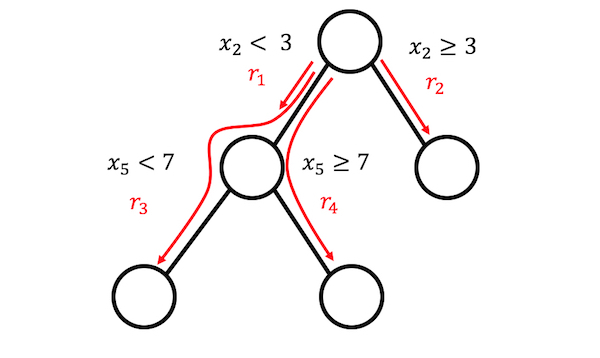
\includegraphics[scale=0.5]{images/rulefit.jpg}
	\label{fig:4_21}
	\caption{Trong cây có 3 nốt cuối này, 4 luật có thể được tạo nên.}
	
\end{figure*}

Vậy ta lấy các cây quyết định này từ đâu? Các cây này được huấn luyện để dự đoán đầu ra mong muốn. Điều này đảm bảo bằng các nhánh sẽ mang thông tin cho bài toán dự đoán. Bất kỳ thuật toán nào mà sinh ra một số lượng cây đều có thể sử dụng trong RuleFit, ví dụ như thuật toán rừng ngẫu nhiên. Mỗi cây có thể được phân tách ra thành các luật quyết định và được dùng như các đặc trưng bổ sung trong các mô hình hồi quy tuyến tính thưa (Lasso).

Trong bài báo về RuleFit, dữ liệu về giá nhà ở Boston mô tả như sau: Mục tiêu là dự đoán giá trị trung vị về giá của các ngôi nhà ở Boston. Một trong các luật được sinh ra bởi RuleFit đó là: IF number of rooms > 6.64 AND concentration of nitric oxide <0.67 THEN 1 ELSE 0.

RuleFit cũng có thể sử dụng độ quan trọng đặc trưng để giúp chỉ ra các thành phần tuyến tính và luật quan trọng cho các dự đoán. Độ quan trọng đặc trưng được tính toán từ các trọng số của mô hình hồi quy. Việc tính toán độ quan trọng có thể được gộp cho các đặc trưng gốc (chưa bị biến đổi và có thể tồn tại trong rất nhiều luật).

RuleFit cũng giới thiệu phác họa phụ thuộc riêng (partial dependence plots) để chỉ ra sự thay đổi trung bình trong dự đoán khi ta thay đổi các đặc trưng. Phác họa phụ thuộc riêng là một phương pháp kiểu mẫu có thể được sử dụng trong bất cứ mô hình nào, và được giải thích trong chương phác họa phụ thuộc riêng (partial dependence plots).

\subsection{Diễn giải và ví dụ}

Do RuleFit ước lượng một mô hình tuyến tính, việc diễn giải giống với các mô hình tuyến tính thông thường. Điều khác biệt duy nhất đó là mô hình có các đặc trưng mới được lấy từ các luật quyết định. Các luật quyết định là các đặc trưng nhị phân: Giá trị 1 nghĩa là tất cả các điều kiện của luật được thỏa mãn và 0 trong trường hợp ngược lại. Với các thành phần tuyến tính trong RuleFit, việc diễn giải giống với mô hình hồi quy tuyến tính: Nếu một đặc trưng tăng một đơn vị, giá trị đầu ra sẽ thay đổi một lượng bằng với giá trị trọng số của đặc trưng đó.

Trong ví dụ này, ta dùng RuleFit để dự đoán số lượng xe được thuê trong một ngày. Bảng sau chỉ ra 5 luật được sinh ra bởi RuleFit bên cạnh các trọng số Lasso và độ quan trọng. Việc tính toán được giải thích ở sau:

\begin{table*}[hbt!]
\centering
\begin{tabular}{|l|l|l|}
\hline
\textbf{Description}                                                  & \textbf{Weight} & \textbf{Imp} \\ \hline
days\_since\_2011 \textgreater 111 \& weathersit in ("GOOD", "MISTY") & 793             & 303                 \\ \hline
37.25 \textless{}= hum \textless{}= 90                                & -20             & 272                 \\ \hline
temp \textgreater 13 \& days\_since\_2011 \textgreater 554            & 676             & 239                 \\ \hline
4 \textless{}= windspeed \textless{}= 24                              & -41             & 202                 \\ \hline
days\_since\_2011 \textgreater 428 \& temp \textgreater 5             & 366             & 179                 \\ \hline
\end{tabular}
\end{table*}

Luật quan trọng nhất đó là: ``days\_since\_2011'' > 111 AND ``weathersit'' in ("GOOD", "MISTY") và trọng số tương ứng là 793. Việc diễn giải đó là: Nếu ``days\_since\_2011'' > 111 AND ``weathersit'' in ("GOOD", "MISTY"), thì số xe được thuê sẽ tăng lên 793 xe, khi tất cả các giá trị đặc trưng khác được giữ nguyên. Về tổng thể, 278 luật được tạo nên từ 8 đặc trưng gốc. Khá nhiều! Nhưng nhờ vào Lasso, chỉ có 58 trong tổng số 278 có giá trị trị trọng số khác 0.

Việc tính toán độ quan trọng của các đặc trưng toàn cục cho thấy nhiệt độ và xu hướng là những đặc trưng quan trọng nhất.

\begin{figure*}[h!]
	\centering
	\includegraphics[scale=0.2]{images/rulefit-importance-1.png}
	\label{fig:4_22}
	\caption{Độ quan trọng của các đặc trưng trong một mô hình RuleFit dự đoán số lượng xe được thuê. Các đặc trưng quan trọng nhất đó là nhiệt độ và xu hướng.}
	
\end{figure*}

Việc tính toán độ quan trọng đặc trưng bao gồm độ quan trọng của các đặc trưng gốc và các luật quyết định trong đó đặc trưng xuất hiện.

\paragraph{Bản mẫu cho việc diễn giải}

Việc diễn giải tương tự với các mô hình tuyến tính: Giá trị đầu ra được dự đoán sẽ thay đổi một lượng $\beta_j$ nếu đặc trưng $x_j$ thay đổi một đơn vị, khi tất cả các đặc trưng còn lại được giữ nguyên. Việc diễn giải trọng số của một luật quyết định khá đặc biệt. Nếu tất cả các điều kiện của luật quyết định $r_k$ được áp dụng, đầu ra dự đoán sẽ thay đổi một lượng $\alpha_k$ (trọng số được học của luật $r_k$ trong mô hình tuyến tính).

Với bài toán phân loại (sử dụng hồi quy logistic thay vì hồi quy tuyến tính): Nếu tất cả các điều kiện được thỏa mãn cho luật $r_k$, tỉ số kỳ dị cho việc một sự kiện xảy ra và không xảy ra sẽ thay đổi một lượng $\alpha_k$ lần.

\subsection{Lý thuyết}

Ta hãy đi sâu hơn vào chi tiết kỹ thuật của thuật toán RuleFit. Thuật toán này bao gồm hai thành phần: Thành phần thứ nhất tạo nên các luật từ các cây quyết định và thành phần thứ hai khớp một mô hình tuyến tính với các đặc trưng gốc và các luật mới như là đầu vào (do đó được gọi là Rule-Fit).

\paragraph{Tạo ra các luật}
Một luật sẽ trông như thế nào? Các luật được sinh ra bởi thuật toán có cấu trúc đơn giản. Ví dụ: IF x2 < 3 AND x5 < 7 THEN 1 ELSE 0. Các luật được xây dựng bằng việc phân tách các cây quyết định: Bất cứ đường nào tới một nốt trong một cây có thể được biến đổi thành một luật quyết định. Các cây được sử dụng cho các luật được khớp để dự đoán đầu ra mong muốn. Do đó, các nhánh và các luật được sinh ra được tối ưu để dự đoán đầu ra ta đang mong muốn. Ta có thể một cách đơn giản kết nối các quyết định nhị phân này (các quyết định nhị phân đưa tới một nốt) với toán tử AND, và voilà, ta có một luật. Tất nhiên ta mong muốn có được nhiều luật mang thông tin cũng như đa dạng. Tăng tốc gradient (gradient boosting) được sử dụng để khớp một tập hợp các cây quyết định bằng việc hồi quy hoặc phân loại giá trị y với các đặc trưng gốc X. Mỗi cây được sinh ra được biến thành rất nhiều luật. Không chỉ với cây tăng tốc, mà bất cứ thuật toán tổ hợp của các cây nào đều có thể được dùng để sinh ra các cây cho thuật toán RuleFit. Một tập hợp cây có thể được mô tả với công thức chung như sau:

$$f(x)=a_0+\sum_{m=1}^M{}a_m{}f_m(X)$$

Trong đó M là số lượng cây và $f_m(x)$ là hàm dự đoán với cây thứ m. Các tham số $\alpha$ là trọng số. Bagged ensembles, random forest, AdaBoost và MART sinh ra các tổ hợp cây và có thể được dùng trong RuleFit.

Ta tạo ra các luật từ các cây của tổ hợp này. Mỗi luật $r_m$ sẽ có dạng:

$$r_m(x)=\prod_{j\in\text{T}_m}I(x_j\in{}s_{jm})$$
với $\text{T}_{m}$ là một tập các đặc trưng được dùng trong cây thứ m, $I$ là hàm báo hiệu trả về 1 khi đặc trưng $x_j$ có mặt trong tập con của các giá trị s cho đặc trưng thứ j (được xác định bởi các nhánh cây) và 0 với các điều kiện còn lại. Với các đặc trưng dạng số, $s_{jm}$ là một khoảng trong dải giá trị của đặc trưng. Một khoảng sẽ có một trong hai dạng như sau: 

$$x_{s_{jm},\text{lower}}<x_j$$

$$x_j<x_{s_{jm},upper}$$

Các nhánh tiếp theo trong đặc trưng đó có thể đưa ta tới các khoảng chia phức tạp hơn. Với các đặc trưng hạng mục, tập con s chứa các hạng mục nhất định của đặc trưng đó.

Một ví dụ cho dữ liệu thuê xe như sau:

$$r_{17}(x)=I(x_{\text{temp}}<15)\cdot{}I(x_{\text{weather}}\in\{\text{good},\text{cloudy}\})\cdot{}I(10\leq{}x_{\text{windspeed}}<20)$$

Luật này trả về giá trị 1 nếu tất cả ba điều kiện được thỏa mãn và trả về 0 trong trường hợp còn lại. Thuật toán RuleFit trích xuất tất cả các luật khả dĩ từ một cây, không chỉ từ các nốt lá. Do đó, một luật khác có thể được tạo ra như sau:

$$r_{18}(x)=I(x_{\text{temp}}<15)\cdot{}I(x_{\text{weather}}\in\{\text{good},\text{cloudy}\}$$

Gộp tất cả lại, số luật có thể được tạo nên từ một tổ hợp M các cây với mỗi nốt cuối $t_m$ là:

$$K=\sum_{m=1}^M2(t_m-1)$$

Một mẹo được giới thiệu bởi RuleFit đó là học các cây với độ sâu ngẫu nhiên để các luật được sinh ra sẽ đa dạng về mặt độ dài. Lưu ý rằng ta loại bỏ các giá trị được dự đoán ở mỗi nốt và chỉ giữ các điều kiện đưa ta tới nốt đó trong khi sinh ra một luật. Trọng số của các luật được quyết định trong bước 2 của RuleFit.

Một cách khác khi xem xét bước 1: Thuật toán RuleFit sinh ra một tập các đặc trưng từ các đặc trưng gốc. Các đặc trưng này là nhị phân và có thể biểu diễn các tương tác khá phức tạp của các đặc trưng gốc. Các luật được chọn để cực đại hóa việc dự đoán. Các luật được sinh ra một cách tự động từ ma trận hiệp biến (covariate matrix) X. Ta có thể xem các luật đơn giản chỉ là các đặc trưng mới dựa trên các đặc trưng gốc.


\paragraph{Mô hình tuyến tính thưa}
Ta có thể có được RẤT NHIỀU luật sau bước 1. Do bước 1 có thể được coi như một bước biến đổi đặc trưng, giờ ta cần khớp mô hình. Tương tự, ta muốn giảm số lượng của các luật. Ngoài các luật, các đặc trưng gốc cũng sẽ được dùng trong mô hình tuyến tính thưa. Tất cả các luật và các đặc trưng gốc trở thành một đặc trưng trong mô hình tuyến tính và nhận một giá trị trọng số. Các đặc trưng gốc được thêm vào bởi vì các cây không thể biểu diễn các mối quan hệ tuyến tính giữa chúng và đầu ra. Trước khi ta huấn luyện một mô hình tuyến tính thưa, ta biến đổi các đặc trưng gốc một chút để mô hình ít bị ảnh hưởng bởi ngoại lai hơn.

$$l_j^*(x_j)=min(\delta_j^+,max(\delta_j^-,x_j))$$

Trong đó $\delta_j^+$ và $\delta_j^-$ là các phân vị của giá trị $\delta$ của phân phối dữ liệu của đặc trưng $x_j$. Ta lựa chọn giá trị $\delta$ là 0.05 nghĩa là với bất cứ giá trị của đặc trưng $x_j$ mà nằm trong khoảng giá trị 5\% thấp nhất hoặc 5\% cao nhất sẽ được đặt về phân vị 5\% hoặc 95\%. Theo kinh nghiệm, giá trị này nên được đặt là 0.025. Thêm vào đó, các thành phần tuyến tính có thể được chuẩn hóa để chúng có độ quan trọng như nhau giống các luật quyết định thông thường.

$$l_j(x_j)=0.4\cdot{}l^*_j(x_j)/std(l^*_j(x_j))$$

Ở đây, 0.4 là giá trị độ lệch chuẩn trung bình của các luật với một phân phối đều $s_k\sim{}U(0,1)$.

Ta gộp cả hai loại đặc trưng để sinh ra một ma trận đặc trưng và huấn luyện mô hình tuyến tính thưa với Lasso như sau:

$$\hat{f}(x)=\hat{\beta}_0+\sum_{k=1}^K\hat{\alpha}_k{}r_k(x)+\sum_{j=1}^p\hat{\beta}_j{}l_j(x_j)$$

Trong đó $\hat{\alpha}$ là vector trọng số được ước lượng cho các đặc trưng tương ứng với luật và $\hat{\beta}$ là vector trọng số cho các đặc trưng gốc. Do RuleFit sử dụng Lasso, hàm mất mát nhận thêm một số thành phần để làm cho các trọng số nhận giá trị 0.

$$(\{\hat{\alpha}\}_1^K,\{\hat{\beta}\}_0^p)=argmin_{\{\hat{\alpha}\}_1^K,\{\hat{\beta}\}_0^p}\sum_{i=1}^n{}L(y^{(i)},f(x^{(i)}))+\lambda\cdot\left(\sum_{k=1}^K|\alpha_k|+\sum_{j=1}^p|b_j|\right)$$

Kết quả của mô hình tuyến tính có các ảnh hưởng tuyến tính cho tất cả các đặc trưng gốc và các luật. Sự diễn giải giống với các mô hình tuyến tính, sự khác nhau duy nhất nằm ở việc các đặc trưng là các luật nhị phân.

\paragraph{Bước 3 (Không bắt buộc) - Độ quan trọng đặc trưng}

Với các thành phần tuyến tính của các đặc trưng gốc, độ quan trọng đặc trưng được tính toán bằng bộ dự đoán chuẩn hóa.

$$I_j=|\hat{\beta}_j|\cdot{}std(l_j(x_j))$$
trong đó $\beta_j$ là trọng số từ mô hình Lasso và $std(l_j(x_j))$ là độ lệch chuẩn của thành phần tuyến tính trên dữ liệu.

Với các thành phần luật quyết định, độ quan trọng được tính bằng công thức sau đây:

$$I_k=|\hat{\alpha}_k|\cdot\sqrt{s_k(1-s_k)}$$
trong đó $\hat{\alpha}_k$ là trọng số Lasso tương ứng của luật và $s_k$ là độ hỗ trợ của đặc trưng trong dữ liệu, được tính bằng tỉ lệ các điểm dữ liệu mà luật quyết định được áp dụng (khi $r_k(x)$ = 0):

$$s_k=\frac{1}{n}\sum_{i=1}^n{}r_k(x^{(i)})$$

Một đặc trưng xuất hiện như một thành phần tuyến tính và cũng trong rất nhiều các luật. Vậy ta làm sao để tính toán độ quan trọng tổng của đặc trưng này. Độ quan trọng $J_j(x)$ của một đặc trưng có thể được tính toán cho từng dự đoán:

$$J_j(x)=I_j(x)+\sum_{x_j\in{}r_k}I_k(x)/m_k$$
trong đó $I_l$ là độ quan trọng của thành phần tuyến tính và $I_k$ là độ uan trọng của các luật quyết định trong đó $x_j$ xuất hiện, và $m_k$ là số đặc trưng tạo nên luật $r_k$. Việc thêm độ quan trọng đặc trưng từ tất cả các điểm dữ liệu cho chũng ta độ quan trọng đặc trưng toàn cục.

$$J_j(X)=\sum_{i=1}^n{}J_j(x^{(i)})$$

Việc lựa chọn một tập con các điểm dữ liệu và tính toán độ ảnh hưởng cho nhóm này là khả dĩ.

\subsection{Ưu điểm}
Thuật toán RuleFit thêm các tương tác giữa các đặc trưng vào các mô hình tuyến tính. Do đó, nó giải quyết vấn đề của mô hình tuyến tính khi ta phải thêm các thành phần tương tác một cách thủ công và cũng mang lại lợi ích khi ta mô hình các quan hệ phi tuyến.

RuleFit có thể giải quyết cả bài toán phân loại và hồi quy.

Các luật được tạo ra dễ dàng có thể diễn giải bởi vì chúng là các luật nhị phân. Mặc cho luật có áp dụng cho một điểm dữ liệu hay không, việc diễn giải tốt chỉ được đảm bảo nếu số điều kiện trong một luật không quá lớn. Một luật với 1 đến 3 điều kiện là khả dĩ, nghĩa là độ sâu của các cây nên có độ sâu lớn nhất là 3.

Thậm chí nếu ta có rất nhiều luật trong một mô hình, chúng không áp dụng cho tất cả các điểm dữ liệu. Với một điểm dữ liệu, chỉ có các luật có trọng số khác 0 được áp dụng. Điều này làm tăng tính khả diễn giải cục bộ.

RuleFit liên quan tới rất nhiều công cụ phân tích và các công cụ này thuộc dạng kiểu mẫu, do đó ta có thể tìm hiểu thêm về chúng tại mục 5.1, 5.4 và 5.5

\subsection{Nhược điểm}

Đôi khi RuleFit tạo ra quá nhiều luật có trọng số khác 0 trong mô hình Lasso. Việc diễn giải do đó cũng bị ảnh hưởng tiêu cực với số lượng tăng dần của các đặc trưng trong mô hình. Một giải pháp hứa hẹn đó là làm cho các ảnh hưởng đặc trưng trở nên đơn điệu, nghĩa là việc tăng giá trị của đặc trưng sẽ dẫn đến một sự tăng tương ứng trong dự đoán.

Tuy nhiên có một vấn đề: Các bài báo cho rằng RuleFit có khả năng làm việc tốt và gần bằng rừng ngẫu nhiên. Tuy nhiên trong một số ít trường hợp khi tôi thử chạy, kết quả không như mong đợi. Hãy thử áp dụng vào bài toán của bạn để kiểm tra điều này.

Kết quả cuối cùng của RuleFit là một mô hình tuyến tính cùng với các đặc trưng đặc biệt (các luật quyết định). Tuy nhiên do nó là mô hình tuyến tính, việc diễn giải các trọng số vẫn trở nên không trực quan. Nó có vấn đề tương tự như mô hình hồi quy tuyến tính khi ta cần có điều kiện tất cả các đặc trưng còn lại là không đổi. Ta cũng gặp một vấn đề nhỏ đó là các luật chồng lên nhau. Ví dụ, một luật cho việc dữ đoán xe là: ``temp > 10'' và một luật khác là ``temp > 15 AND weather = GOOD''. Nếu thời tiết tốt và nhiệt độ lớn hơn 15 độ thì mặc nhiên nhiệt độ sẽ lớn hơn 10 độ. Trong các trường hợp khi luật thứ hai được áp dụng, luật thứ nhất cúng sẽ có hiệu lực. Sự diễn giải của các trọng số ước lượng cho luật thứ hai đó là: ``Giả sử mọi đặc trưng cố định, giá trị xe được dự đoán sẽ tăng lên $\beta_2$ lần khi thời tiết tốt và nhiệt độ lớn hơn 15''. Tuy nhiên, rõ ràng rằng giả thiết ``các đặc trưng là không đổi có vấn đề, bởi vì nếu luật thứ 2 được áp dụng, thì luật thứ nhất cũng vậy và việc diễn giải trở nên vô nghĩa.

\subsection{Các phương pháp khác và các gói phần mềm}

Thuật toán RuleFit được triển khai với R bởi Fokkema and Christoffersen (2017) và bạn có thể tìm hiểu thêm một triển khai khác trên Github ở \href{https://github.com/christophM/rulefit}{đây}.

Một thuật toán khá giống RuleFit gọi là \href{https://github.com/scikit-learn-contrib/skope-rules}{skope-rules}, một mô đun Python cũng trích xuất các luật từ các tổ hợp. Tuy nhiên cách học các luật là khác nhau: Đầu tiên, skope-rules sẽ loại bỏ các luật ít được sử dụng dựa trên các ngưỡng về recall và precision. Sau đó, các luật tương đồng và trùng lặp sẽ được loại bỏ bằng cách thực hiện một phương pháp lựa chọn dựa trên tính đa dạng của các thành phần logic (biến + các toán tử lớn/nhỏ hơn) và hiệu năng (F1 score) của các luật. Bước cuối này không phụ thuộc vào việc sử dụng Lasso, nhưng chỉ cân nhắc F1 score và các thành phần logic tạo nên các luật.

\section{Các mô hình khả diễn giải khác}

Danh sách các mô hình khả diễn giải được mở rộng liên tục. Nó bao gồm các mô hình đơn giản ví dụ như mô hình tuyến tính, cây quyết định và Naive Bayes, nhưng cũng tồn tại các mô hình phức tạp hơn bao gồm (hoặc biến thể) từ các mô hình học máy bất khả diễn giải nhưng đã được trang bị tính khả diễn giải. Đặc biệt, các công bố khoa học trong loại mô hình thứ hai đang được đẩy mạnh và rất khó để nắm bắt xu thế. Cuốn sách này chỉ bao gồm bộ phân loại Naive Bayes và k hàng xóm gần nhất.

\subsection{Bộ phân loại Naive Bayes}

Bộ phân loại Naive Bayes sử dụng định lý Bayes về xác suất có điều kiện. Với từng đặc trưng, nó tính toán xác suất cho một lớp phụ thuộc vào giá trị của đặc trưng. Bộ phân loại Naive Bayes tính toán các xác suất cho các lớp với từng đặc trưng đơn lẻ, tương đương với một giả thiết mạnh (strong = naive) về tính phụ thuộc  của các đặc trưng. Naive Bayes là một mô hình xác suất có điều kiện và nó mô hình xác suất của một lớp $C_k$ như sau:

$$P(C_k|x)=\frac{1}{Z}P(C_k)\prod_{i=1}^n{}P(x_i|C_k)$$

Thành phần Z là tham số hiệu chỉnh để đảm bảo rằng tổng các xác suất luôn là 1 (nếu không chúng sẽ không phải là các giá trị xác suất). Xác suất có điều kiện của một lớp là xác suất của lớp đó nhân với xác suất của từng đặc trưng trong lớp, được chuẩn hóa bởi tham số Z. Công thức này có thể được suy ra bằng cách sử dụng định lý Bayes.

Naive Bayes là một dạng mô hình khả diễn giải bởi giả thiết về tính phụ thuộc của các đặc trưng. Nó có thể được diễn giải ở mức mô đun. Với mỗi đặc trưng,  việc chúng ảnh hưởng tới một dự đoán như thế nào là khá rõ ràng, do đó ta có thể diễn giải xác suất có điều kiện này.

\subsection{K hàng xóm gần nhất}

K hàng xóm gần nhất là một phương pháp có thể được sử dụng trong cả bài toán hồi quy và phân loại, chúng sử dụng các hàng xóm của một điểm dữ liệu để đưa ra dự đoán. Với bài toán phân loại, thuật toán này gán lớp hay xuất hiện nhất của các hàng xóm gần nhất cho một điểm dữ liệu. Với bài toán hồi quy, nó lấy trung bình của đầu ra ứng với các hàng xóm. Điều khó khăn trong thuật toán này đó là việc tìm ra số lượng k và quyết định làm sao để tính toán khoảng cách giữa các điểm dữ liệu, điều mà sẽ định nghĩa các hàng xóm.

Mô hình này khác với các mô hình khả diễn giải khác trong cuốn sách này ở chỗ nó là một thuật toán học dựa trên các điểm dữ liệu (instance-based learning). Vậy làm sao để ta diễn giải mô hình này? Đầu tiên, ta cần lưu ý rằng không có tham số nào được học, do đó sẽ không có việc diễn giải ở mức mô đun. Hơn nữa, ta không thể diễn giải mô hình ở mức toàn cục bởi vì mô hình là cục bộ và không tồn tại trọng số hay cấu trúc toàn cục nào được học cả. Có lẽ ta có thể diễn giải ở mức cục bộ? Để giải thích một dự đoán, ta luôn có thể lấy ra được k hàng xóm được dùng cho việc dự đoán. Liệu mô hình có khả diễn giải hay không phụ thuộc vào câu hỏi liệu ta có thể diễn giải các điểm dữ liệu trong tập dữ liệu hay không. Nếu một điểm dữ liệu bao gồm hàng trăm thậm chí hàng ngàn đặc trưng, ta rõ ràng không thể diễn giải. Nhưng nếu ta chỉ có vài đặc trưng hoặc tồn tại phương pháp để làm giảm số đặc trưng về một tập nhỏ các đặc trưng quan trọng nhất, việc trình bày k điểm dữ liệu hàng xóm có thể cho ta các giải thích tốt.
